%*********************************************************************
%*************************** Main Document ***************************
%*********************************************************************

% Header includes document class and packages
%***********************************************************************
%*************************** Document Header ***************************
%***********************************************************************


% Document formatting
\documentclass[a4paper,11pt]{article} %document type
\usepackage[a4paper, left=3cm, right=2.5cm, bottom=2.5cm]{geometry}  %borders
\usepackage{fancyhdr} %pagestyle
\setlength{\headheight}{15pt} %page header height
\usepackage[normalem]{ulem} %underline not only with line (eg. dotty )
\usepackage{amsfonts}	%Für Schriftarten
\usepackage[onehalfspacing]{setspace} %linespace
\usepackage{indentfirst} %ersten Paragraph des Kapitels einrücken

% Character set and orthography
\usepackage[utf8]{inputenc} %UTF8, also mit Umlauten
\usepackage[ngerman]{babel}	%Deutsche Rechtschreibung
\usepackage[T1]{fontenc}	%Westeuropäische Codierung

% Graphics
\usepackage{graphicx}
\usepackage{float} %[H] for placement forcing
\usepackage{caption} %captionsetup

% Acronyms
\usepackage[printonlyused]{acronym}

% References
\usepackage{titleref} %for \ref
\usepackage[colorlinks=true,urlcolor=blue,linkcolor=black,citecolor=black]{hyperref}

% URL
\usepackage{url} 
\newcommand*\oldurlbreaks{}
\let\oldurlbreaks=\UrlBreaks
\renewcommand{\UrlBreaks}{\oldurlbreaks\do\a\do\b\do\c\do\d\do\e%
  \do\f\do\g\do\h\do\i\do\j\do\k\do\l\do\m\do\n\do\o\do\p\do\q%
  \do\r\do\s\do\t\do\u\do\v\do\w\do\x\do\y\do\z\do\?\do\&\do\-}
 
 
  
%\usepackage{ragged2e}	%justification (block)
%\PassOptionsToPackage{hyphens}{url}
%\usepackage{scrextend} %Koma Blocksatz
%\usepackage{tabularx} %Tabellen verwenden

%\usepackage[numbers]{natbib} %Für deutsches Literaturverzeichnis

%\usepackage{blindtext}
\usepackage{siunitx}
\sisetup{locale = DE}
\usepackage{tikz}
\usetikzlibrary{shapes.geometric, arrows}
\usetikzlibrary{calc} 
\tikzstyle{startstop} = [rectangle, rounded corners, minimum width=3cm, minimum height=0.5cm,text centered, draw=black, fill=red!30]

\tikzstyle{process} = [rectangle, minimum width=3cm, minimum height=0.5, text centered, text width=3cm, draw=black, fill=orange!30]

\tikzstyle{io} = [trapezium, trapezium left angle=70, trapezium right angle=110, minimum width=3cm, minimum height=0.5, text centered, text width=2cm, draw=black, fill=blue!30]

\tikzstyle{decision} = [diamond, minimum width=3cm, minimum height=0.5, text centered, draw=black, fill=green!30]

\tikzstyle{arrow} = [thick,->,>=stealth]

\usepackage[european]{circuitikz}
%\usepackage{enumitem,amssymb}
%\newlist{checklist}{itemize}{2}
%\setlist[checklist]{label=$\square$}

\begin{document}

\pagenumbering{Alph} % Intern werden die Ersten seiten mit Alpha-Stiel nummeriert um Doppelreferenzen zu vermeiden 

% Titlepage
%*****************************************************************
%*************************** Titlepage ***************************
%*****************************************************************

\begin{titlepage}
\begin{center}

%Logo
\begin{figure}[H]

\includegraphics[width=15cm]{titlepage/images/Logo_HAW_Landshut} 
\end{figure}\textnormal{ }\\[0.1cm]

%Company and departement/faculty
\textbf{\large{HOCHSCHULE FÜR ANGEWANDTE\\[0.5cm] WISSENSCHAFTEN LANDSHUT}}\\[1.0cm]
\textsc{\large {Fakultät Elektrotechnik und Wirtschaftsingenieurwesen}}\\[1.0cm]
\textnormal{{Masterstudium}}\\[0.5cm]
\textnormal{{Elektrotechnik}}\\[1.0cm]

%Type of document
\Large\textbf{Projektbericht}\\[0.5cm]
\large{Eingebettete Autonome Systeme}\\[0.5cm]

%Title of the article
\large\textbf {Aufbau und Programmierung eines Modellfahrzeugs
für den NXP Cup Gesamtdokumentation}\\[1.5cm]

%Authors and release date
\small\textnormal{vorgelegt von:}\\[0.3cm]
\textnormal{Ambrosch Markus, Ecker Christian, Summer Matthias}\\[0.3cm]
\textnormal eingereicht am:\\[0.3cm]
\textnormal{30.07.2021}

%Bottom of the page
\vfill

%Supervisor
\textnormal{Betreuer: Prof. Dr. Mathias Rausch} 

\end{center}
\end{titlepage}
\newpage

% Set page counter to 2 and page numbering to Roman
\pagenumbering{Roman}
\setcounter{page}{2}

% Section 0 Inhalt
%*****************************************************************
%*************************** Section 0 ***************************
%**************************** Vorwort ****************************
%*****************************************************************


\pagestyle{fancy}
\rhead{\thepage} \chead{} \lhead{\nameref{Sec0}}
\cfoot{}


\addcontentsline{toc}{section}{Vorwort}
\section*{Vorwort}\label{Sec0}

Dieser Projektbericht enthält zusätzlich zur Dokumentation der im Sommersemester 2021 erzielten Ergebnisse auch die des Vorsemesters (Wintersemester 2020/2021). Nachdem im Wintersemester nicht alle der gesetzten Ziele erreicht werden konnten, stellt dieser Bericht die Gesamtdokumentation des über zwei Semester andauernden Projekts \glqq{}Aufbau und Programmierung eines Modellfahrzeugs für den NXP Cup\grqq{} dar.\vspace{11pt} 

Zur Unterstützung bei der Erledigung der noch ausstehenden Aufgaben ist zum Sommersemester Herr Markus Ambrosch dem Projekt-Team des Wintersemesters (Ecker Christian \& Summer Matthias) beigetreten.\vspace{11pt} 

***Arne Kullina danken***\vspace{11pt} 
***Rausch danken***\vspace{11pt} 

\newpage
%***************************Muss noch probegelesen werden
%***************************Dank schreiben

% Table of contents
%*************************************************************************
%*************************** Table of contents ***************************
%*************************************************************************


\pagestyle {fancy}
\rhead{\thepage} \chead{} \lhead{Inhaltsverzeichnis}
\cfoot{}

\addcontentsline{toc}{section}{Inhaltsverzeichnis}
\tableofcontents 

\newpage

% Table of acronyms
%****************************************************************
%*************************** Acronyms ***************************
%****************************************************************


\pagestyle {fancy}
\rhead{\thepage} \chead{} \lhead{Abkürzungsverzeichnis}
\cfoot{}

\addcontentsline{toc}{section}{Abkürzungsverzeichnis}
\section*{Abkürzungsverzeichnis}

\begin{acronym}[ABS-Kunststoff]
	\acro{BLDCMot}[BLDC-Motor]{Brushless Direct Current Motor}
	\acroplural{BLDCMot}[BLDC-Motoren]{Brushless Direct Current Motoren}
	\acro{DCMot}[DC-Motor]{Gleich\-strom\-motor}
	\acroplural{DCMot}[DC-Motoren]{Gleich\-strom\-motoren}
	\acro{RC}[RC]{Remote-Control}
	\acro{ESC}[ESC]{Electronic Speed Controller}
	\acro{PWM}[PWM]{Puls\-weiten\-modulation}
	\acro{NXP}[NXP]{Next Experience}
	\acro{CPU}[CPU]{Central Processing Unit}
	\acro{ABS}[ABS-Kunststoff]{Acrylnitril-Butadien-Styrol Copolymer}
	\acro{SLA}[SLA-Drucker]{3D-Drucker mit Stereolithographie-Verfahren}
	\acro{OLED}[OLED-Display]{organisches Leuchtdioden-Display}
	\acro{I2C}[I2C]{Inter Integrated-Circuit}
	\acro{RAM}[RAM]{Random-Access Memory}
	\acro{DMA}[DMA]{Direct Memory Access}
	\acro{EEPROM}[EEPROM]{Electrically Erasable Programmable Read-Only Memory}
\end{acronym}

\newpage


% Saving page counter value for attachement
\newcounter{pagecountersaving}
\setcounter{pagecountersaving}{\value{page}}

% Set page counter to 1 and page numbering to arabic
\pagenumbering{arabic}
\setcounter{page}{1}

% Section 1 Einführung
%*****************************************************************
%*************************** Section 1 ***************************
%************************** Einfuehrung **************************
%*****************************************************************


%\pagestyle{fancy}
\rhead{\thepage} \chead{} \lhead{\ref{Sec1}. \nameref{Sec1}}
\cfoot{}

\section{Einführung}\label{Sec1}

\subsection{Zielsetzung}\label{Sub1Sec1}

Das Ziel der Projektarbeit ist der Aufbau und die Programmierung eines Modellfahrzeugs für den \ac{NXP}-Cup mit einem eigens gebauten, selbstfahrenden Fahrzeug. Bei diesem Wettbewerb müssen die im Maßstab 1:18 angefertigten Fahrzeuge einen Parcours in möglichst kurzer Zeit selbstständig durchfahren. Diese werden von Studenten aus Europa, dem mittleren Osten und Afrika auf Grundbasis eines Bausatzes entwickelt. Die Fahrbahn wird von zwei schwarzen Streifen begrenzt, die auf einem weißen Hintergrund aufgebracht sind. Das Fahrzeug muss diese Begrenzungen erkennen und anhand deren Auswertung die Geschwindigkeit des Fahrzeugs und dessen Lenkwinkel anpassen. Angetrieben wird das Auto mithilfe zweier \acp{BLDCMot}. Die Lenkung wird mittels Servoantrieb und Lenkgestänge realisiert. Auf dem Fahrzeug dürfen beliebig viele Prozessoren und Bauteile von NXP Semiconductors, welche den Wettbewerb ausrichten, verwendet werden~\cite{MWil}. Sind für das eigene Fahrzeug benötigte Komponenten nicht im Portfolio von NXP Semiconductors vorzufinden, können auch eigene oder die Produkte anderer Hersteller verwendet werden. 

\subsection{Konzept}\label{Sub1Sec2}

Zu Beginn soll das Fahrzeug zuerst mit dem Standardbausatz zusammengebaut werden. Die Software wird aus bereits vorhandenen, vorherigen Projekten zusammengesetzt und optimiert. Ein großes Augenmerk liegt dabei auf einem übersichtlicheren Aufbau des Programms und besserer Nachvollziehbarkeit durch Kommentation und eingängigerer Benennung der Funktionen und Parameter.\vspace{11pt}

Die Programmierung soll Stück für Stück vorgenommen werden. Zu Beginn wird die Ansteuerung der \acp{BLDCMot} bearbeitet. Ist der Punkt erreicht, an dem die Motoren angesteuert und die Drehzahl über die Puls-Weiten-Modulation variiert werden kann, soll eine Möglichkeit der Drehzahlerkennung erarbeitet werden. Im Anschluss an die Inbetriebnahme der Antriebe wird die Software für den Servomotor der Lenkung erstellt. Die Bedienung des Fahrzeugs soll über ein Display und einen Dreh-Encoder realisiert werden. Zur Streckenerkennung wird eine Zeilenkamera verwendet. Bei Bedarf kann zusätzlich oder ersatzweise eine größere Kamera eingesetzt werden. Nach der Inbetriebnahme der Einzelkomponenten werden deren Ansteuerung und Auswertung mithilfe einer Regelung verknüpft. Die Software des Fahrzeugs soll am Ende so optimiert werden, dass es schnellstmöglich, aber auch sicher durch den Parcours fährt.\vspace{11pt}

Nach der erfolgreichen Entwicklung des Fahrzeugs für das Durchfahren des Parcours soll für eine zusätzliche Wettbewerbsdisziplin eine Objektdetektion mithilfe eines Ultraschallboards realisiert werden, welches bereits in den vorherigen Semestern von anderen Studierenden entwickelt wurde. Mithilfe dieses Ultraschall-Boards soll das Fahrzeug Hindernisse erkennen und um diese herumfahren können.\vspace{11pt}

Karosserieteile, wie beispielsweise eine  Akkuhalterung oder eine Stoßstange mit der Möglichkeit zur Befestigung des Ultraschallboards, werden mit einem 3D-Druck-Verfahren erstellt. Dafür werden vor allem Teile gedruckt, welche bereits von Herrn Arne Kullina im Rahmen seines Praktikums bei Herrn Prof. Dr. Mathias Rausch im Sommersemester 2020 konstruiert wurden. Für eine übersichtlichere Kabelführung und einfachere De- und Montage wird eine Lochrasterplatine mit Steckkontakten erstellt, an welchen die Einzelmodule angeschlossen werden können.

\newpage
%***************************Änderungen in Zielsetzung und Konzept müssen noch probegelesen werden!!

% Section 2 Aufbau des Fahrzeugs
%*****************************************************************
%*************************** Section 2 ***************************
%********************* Aufbau des Fahrzeugs **********************
%*****************************************************************


\pagestyle{fancy}
\rhead{\thepage} \chead{} \lhead{\ref{Sec2}. \nameref{Sec2}}
\cfoot{}

\section{Aufbau des Fahrzeugs}\label{Sec2}

\subsection{Grundaufbau}\label{Sec2Sub1}

Das Fahrzeug besteht zum größten Teil aus einem Standarbausatz. Auf der unteren Ebene, der Grundplatte, sind die \acp{BLDCMot} für den Antrieb, der Servomotor und die Reifen montiert (siehe Abbildung \ref{fig:Grundplatte01}). In einem weiteren Schritt werden hier auch die Anbauteile des Fahrzeugs aus dem 3D-Druck befestigt, wie beispielsweise die Stoßstange und die Seitenschweller (näheres in Kapitel \ref{Sec2Sub2}).

\begin{figure}[H] %H für Positionierung hier
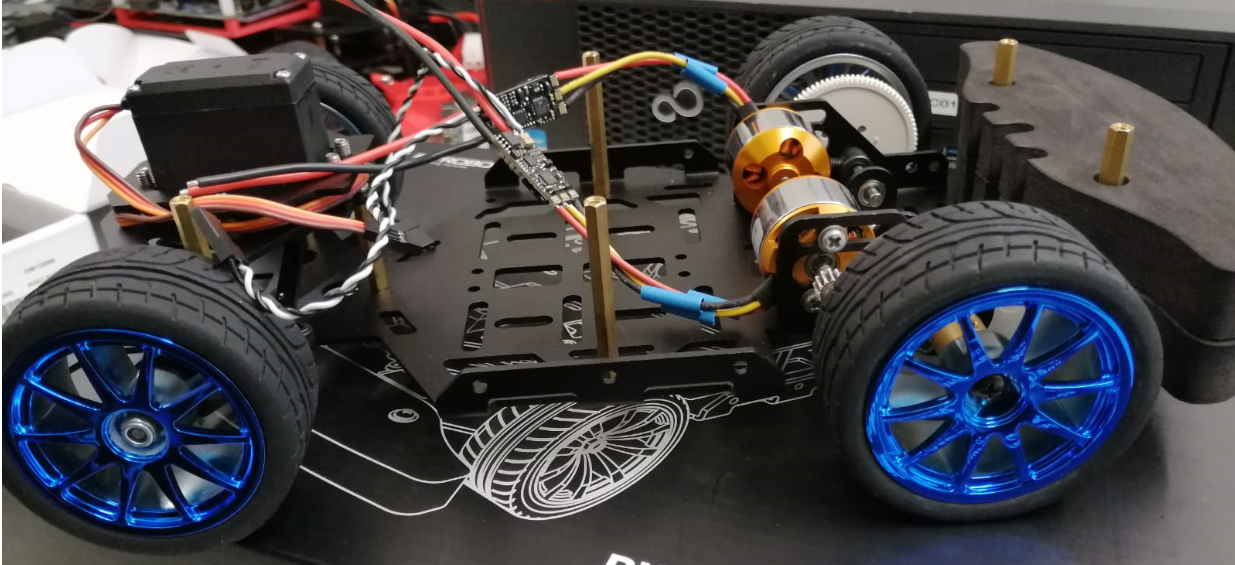
\includegraphics[width=.90\textwidth]{sec2/images/Grundaufbau/Grundplatte01} 
\centering
\captionsetup{width=.95\textwidth}
\caption[Grundplatte des Standardbausatzes für das Fahrzeug]{Grundplatte des Standardbausatzes für das Fahrzeug mit BLDC-Motoren, Motorcontrollern, Servomotor und Reifen}\centering
\label{fig:Grundplatte01}
\end{figure}

\begin{figure}[H] %H für Positionierung hier

\includegraphics[width=.90\textwidth]{sec2/images/Grundaufbau/Grundplatte02} 
\centering
\captionsetup{width=.95\textwidth}
\caption[Grundplatte des Fahrzeugs]{Grundplatte des Fahrzeugs mit Akku, Strom-Verteilerplatine und bereits montierter Fahrzeug-Peripherie}\centering
\label{fig:Grundplatte02}
\end{figure}

Auf der Grundplatte ist zusätzlich eine Verteilerplatine für die Batteriespannung montiert. Auch der Akku findet auf dieser Ebene seinen Platz (siehe Abbildung \ref{fig:Grundplatte02}). Die Steckmöglichkeiten für alle Komponenten des Fahrzeugs werden, anders als bei Herrn Kullinas Fahrzeug, nicht auf der Grundplatte realisiert, sondern auf der oberen Ebene. Dass auf der Grundplatte nur noch Komponenten Platz finden, zu denen man selten Zugang benötigt, hat den Vorteil, dass man das Fahrzeug nur noch in Ausnahmefällen auseinandernehmen muss.\vspace{11pt}

Oberhalb der Grundplatte des Fahrzeugs, auf der die Antriebe, die Lenkung, die 3D-Druck Anbaukomponenten und der Akku platziert sind, wird mit einer weiteren Montageplatte eine zweite Ebene aufgespannt (siehe Abbildung \ref{fig:ObereEbene01}). Auf dieser oberen Ebene werden der Controller mit dem Bedienungsboard, die Kamera und die Verteilerplatine mit Steckmöglichkeiten für die Fahrzeugkomponenten montiert (siehe Abbildung \ref{fig:ObereEbene02}).

\begin{figure}[H] %H für Positionierung hier
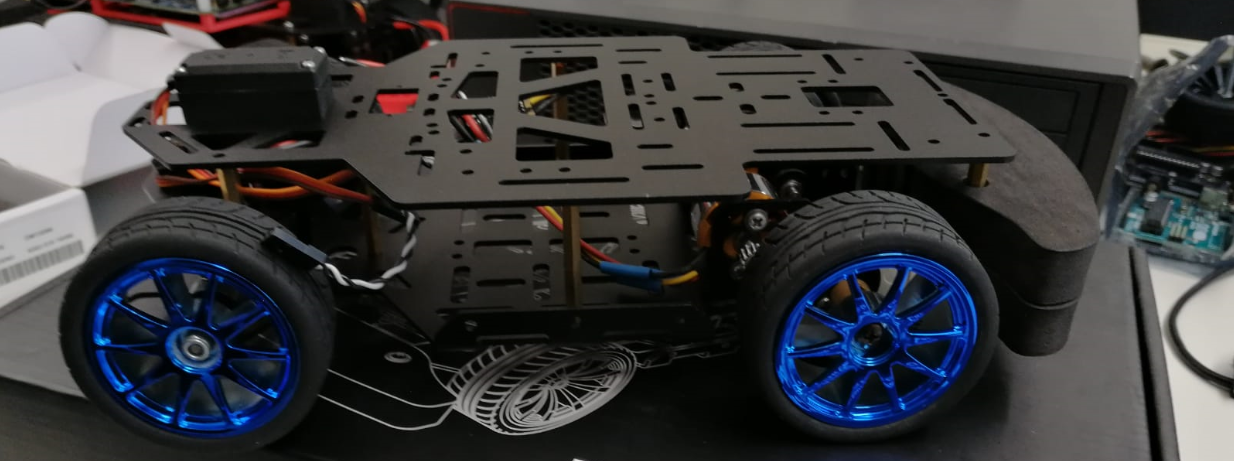
\includegraphics[width=.86\textwidth]{sec2/images/Grundaufbau/ObereEbene01} 
\centering
\captionsetup{width=.92\textwidth}
\caption[Obere Ebene des Standardbausatzes für das Fahrzeug]{Obere Ebene des Standardbausatzes für das Fahrzeug ohne Montage des Controllers und der Kamera}\centering
\label{fig:ObereEbene01}
\end{figure}

\begin{figure}[H] %H für Positionierung hier

\includegraphics[width=.75\textwidth]{sec2/images/Grundaufbau/ObereEbene02} 
\centering
\captionsetup{width=.95\textwidth}
\caption[Obere Ebene des Fahrzeugs]{Obere Ebene des Fahrzeugs mit Controller, Bedienungsboard, Kamera und Verteilerplatine}\centering
\label{fig:ObereEbene02}
\end{figure}

\newpage

\subsection{Anbaukomponenten aus dem 3D-Druck}\label{Sec2Sub2}

Zusätzlich zum Standardbausatz werden auch Anbaukomponenten verbaut, die mithilfe eines 3D-Druckers gefertigt und dann am Fahrzeug angebracht werden. Die Folgekapitel zeigen alle gedruckten Einzelteile und erläutern deren Zweck näher. Die Anbauteile wurden größtenteils von Herrn Arne Kulinna konstruiert, der im Rahmen eines Praktikums bei Herrn Prof. Dr. Mathias Rausch an der Hochschule Landshut bereits eine erste Version des Fahrzeugs mit demselben Bausatz erstellt hat.

\subsubsection{Stoßstange und Ultraschallboard-Halterung}\label{Sec2Sub2SubSub1}

Das Fahrzeug benötigt eine Stoßstange, damit bei der Kollision mit einem Hindernis kein wichtiges Teil des Fahrzeugs, wie beispielsweise der Servo-Motor oder das Ultraschall-Board, beschädigt wird. Da das zur Hinderniserkennung zu verwendende Ultraschallboard frontal befestigt wird, müssen in der Stoßstange kegelförmige Aussparungen eingeplant werden, damit die Stoßstange nicht fälschlicherweise als Hindernis erkannt wird. In den Abbildungen \ref{fig:StossstangeKonstruktion01} und \ref{fig:StossstangeKonstruktion02} sind die Konstruktionsbilder der beiden Stoßstangenteile abgebildet.

\begin{figure}[H] %H für Positionierung hier
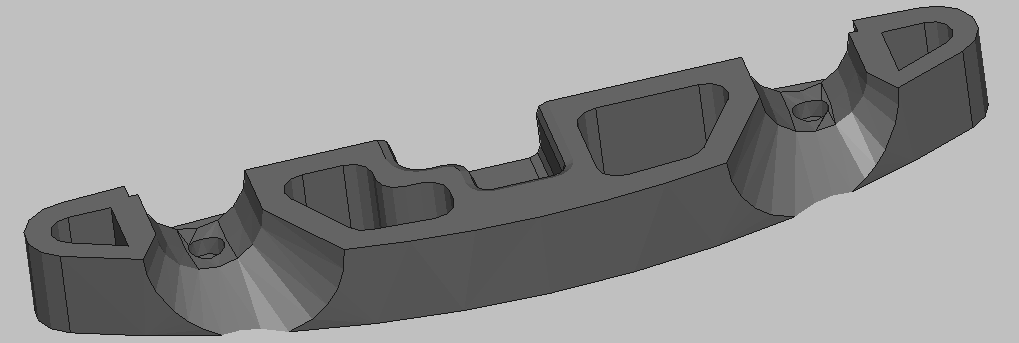
\includegraphics[width=.8\textwidth]{sec2/images/3DAnbaukomponenten/Konstruktionsbilder/StossstangeKonstruktion01} 
\centering
\captionsetup{width=.95\textwidth}
\caption[Konstruktionsbild des oberen Stoßstangenteils]{Konstruktionsbild des oberen Stoßstangenteils}\centering
\label{fig:StossstangeKonstruktion01}
\end{figure}

\begin{figure}[H] %H für Positionierung hier
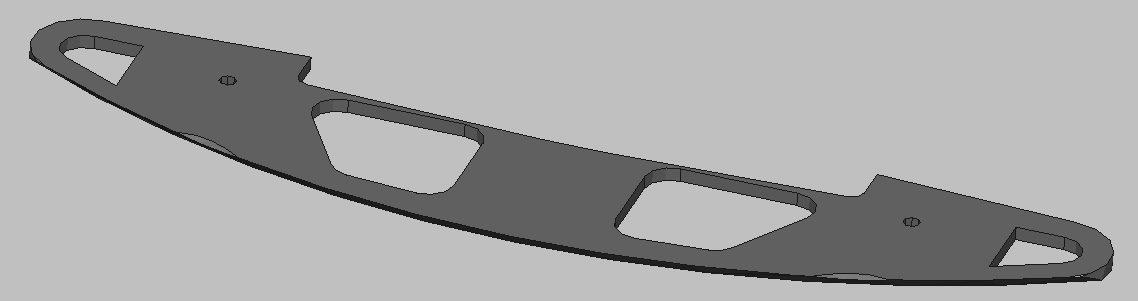
\includegraphics[width=.8\textwidth]{sec2/images/3DAnbaukomponenten/Konstruktionsbilder/StossstangeKonstruktion02} 
\centering
\captionsetup{width=.95\textwidth}
\caption[Konstruktionsbild des unteren Stoßstangenteils]{Konstruktionsbild des unteren Stoßstangenteils}\centering
\label{fig:StossstangeKonstruktion02}
\end{figure}

Abbildung \ref{fig:StossstangeDruck} zeigt die fertig gedruckten Stoßstangenkomponenten. Der untere, flache Teil der Stoßstange wird mit zwei Schrauben an der oberen Komponente befestigt. Die gesamte Stoßstange wird ebenfalls an nur zwei Stellen mit der Karosserie verbunden. Zusätzlichen Halt bekommt die Stoßstange von der Halterung des Ultraschallboards.

\begin{figure}[H] %H für Positionierung hier
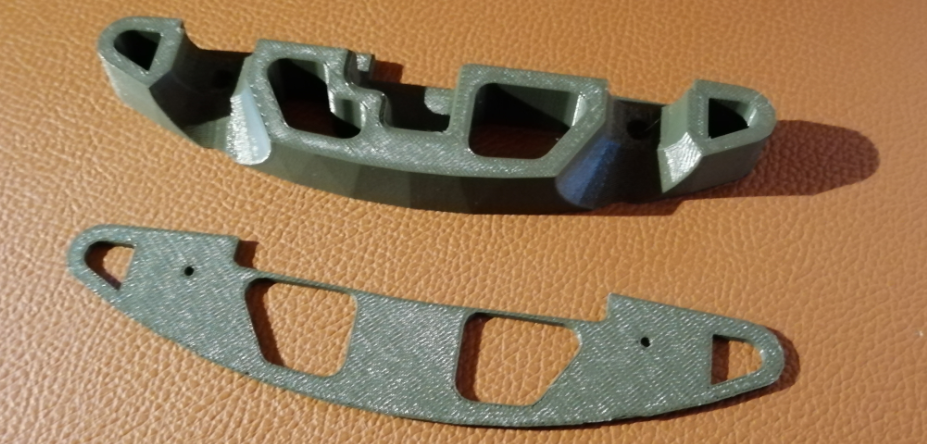
\includegraphics[width=.7\textwidth]{sec2/images/3DAnbaukomponenten/Druckbilder/StossstangeDruck} 
\centering
\captionsetup{width=.95\textwidth}
\caption[Gedrucktes oberes und unteres Stoßstangenteil]{Gedrucktes oberes und unteres Stoßstangenteil}\centering
\label{fig:StossstangeDruck}
\end{figure}


Wie bereits erwähnt, wird das Ultraschallboard frontal am Fahrzeug montiert. Dazu wird eine Aufnahme benötigt, an welcher das Board befestigt werden kann. In den Abbildungen \ref{fig:UltraschallHalterungKonstruktion} und \ref{fig:UltraschallHalterungDruck} sind die Konstruktionszeichnung und die fertig gedruckte Halterung abgebildet.

\begin{minipage}[b]{0.4\textwidth}
\centering
\begin{figure}[H] %H für Positionierung hier
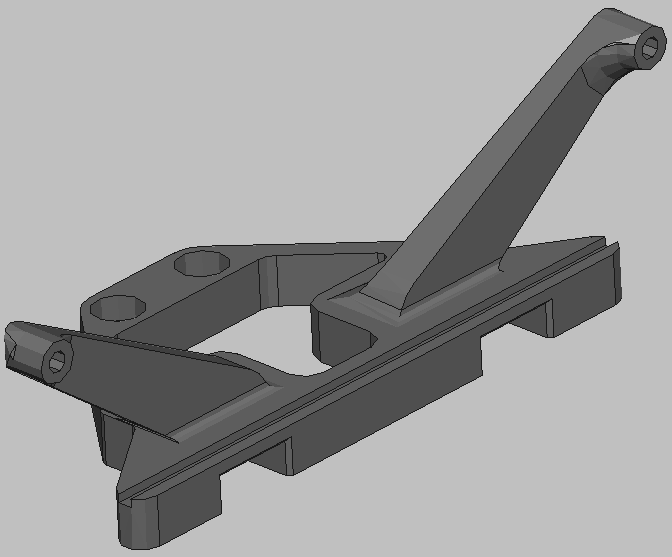
\includegraphics[width=.9\textwidth]{sec2/images/3DAnbaukomponenten/Konstruktionsbilder/UltraschallHalterungKonstruktion} 
\centering
\captionsetup{width=.95\textwidth}
\caption[Konstruktionsbild der Halterung des Ultraschallboards]{Konstruktionsbild der Halterung des Ultraschallboards}\centering
\label{fig:UltraschallHalterungKonstruktion}
\end{figure}
\end{minipage}
\begin{minipage}[b]{0.54\textwidth}
\begin{figure}[H] %H für Positionierung hier
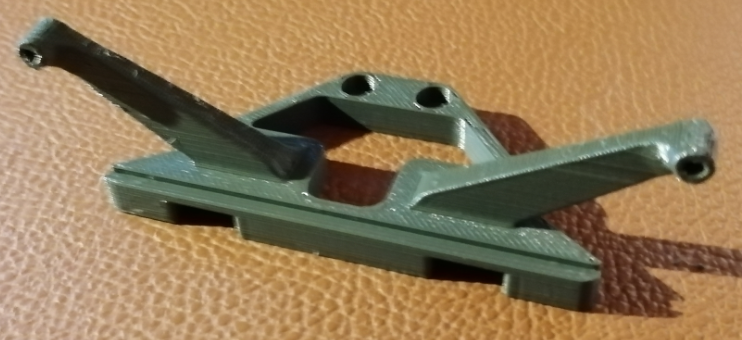
\includegraphics[width=.9\textwidth]{sec2/images/3DAnbaukomponenten/Druckbilder/UltraschallHalterungDruck} 
\centering
\captionsetup{width=.95\textwidth}
\caption[Gedruckte Halterung des Ultraschallboards]{Gedruckte Halterung des Ultraschallboards}\centering
\label{fig:UltraschallHalterungDruck}
\end{figure}
\end{minipage}
\vspace{4mm}

In den Abbildung \ref{fig:StossstangeUltraschallHalterungMontage01} und \ref{fig:StossstangeUltraschallHalterungMontage02} sind die am Fahrzeug fertig montierte Stoßstange und Ultraschallboard-Halterung abgebildet. Die Stellen, an denen diese Bauteile am Fahrzeug fixiert sind, sind in den Abbildungen farblich hervorgehoben. 

\begin{figure}[H] %H für Positionierung hier
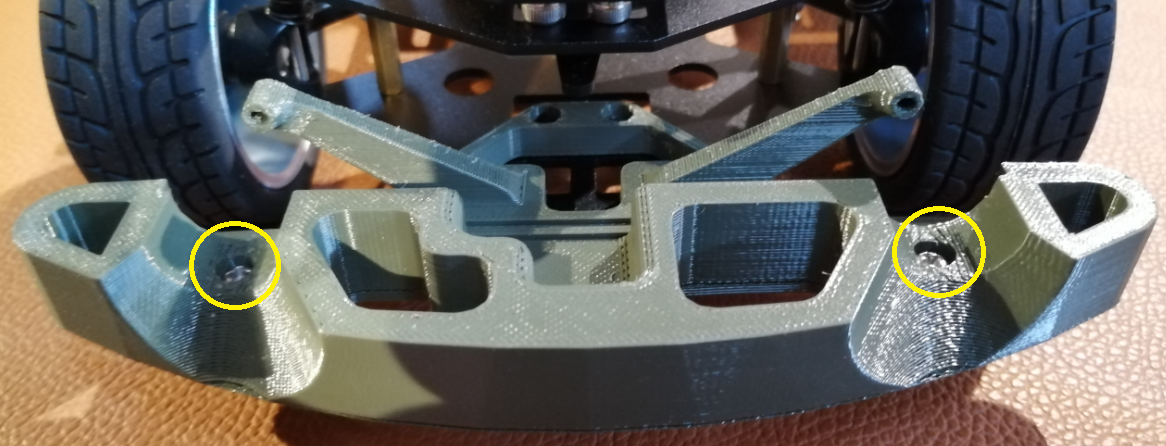
\includegraphics[width=.78\textwidth]{sec2/images/3DAnbaukomponenten/Montagebilder/StossstangeUltraschallHalterungMontage01} 
\centering
\captionsetup{width=.95\textwidth}
\caption[Draufsicht der Stoßstange und der Ultraschallboard-Halterung]{Draufsicht der Stoßstange und der Ultraschallboard-Halterung; Befestigungsschrauben der unteren Stoßstangenkomponente in gelb}\centering
\label{fig:StossstangeUltraschallHalterungMontage01}
\end{figure}

\begin{figure}[H] %H für Positionierung hier
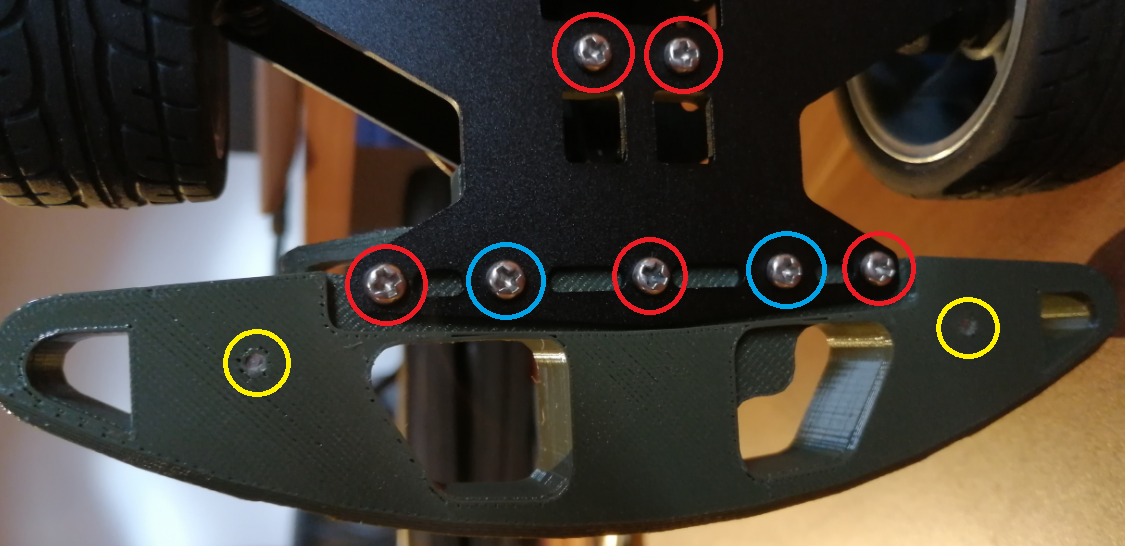
\includegraphics[width=.7\textwidth]{sec2/images/3DAnbaukomponenten/Montagebilder/StossstangeUltraschallHalterungMontage02} 
\centering
\captionsetup{width=.95\textwidth}
\caption[Untersicht der Stoßstange und der Ultraschallboard-Halterung]{Untersicht der Stoßstange und der Ultraschallboard-Halterung; Befestigungsschrauben der Stoßstange in blau, Schrauben der Ultraschallboard-Halterung in rot und Schrauben zur Befestigung der unteren Stoßstangenkomponente in gelb}\centering
\label{fig:StossstangeUltraschallHalterungMontage02}
\end{figure}

\subsubsection{Akku-Halterung und Seitenschweller}\label{Sec2Sub2SubSub2}

Der Akku für das Fahrzeug soll auf der unteren Ebene Platz finden, um den Schwerpunkt des Fahrzeugs niedrig zu halten. Damit der Akku einen festen Sitz hat und nicht beim Gasgeben oder Bremsen verrutscht, wird auf der unteren Ebene in der Mitte eine Halterung installiert (Konstruktionszeichnung in Abbildung \ref{fig:AkkuHalterungKonstruktion}). Die Akku-Halterung fungiert auch als Kabeldurchführung, damit die Drähte und Kabel sauber gebündelt werden können und nicht frei in der Luft geführt werden. In Abbildung \ref{fig:AkkuHalterungDruck} ist die fertig gedruckte Akku-Halterung zu sehen. Die Halterung wird von unten mit 4 Schrauben auf der Grundplatte des Fahrzeugs montiert.

\begin{minipage}[b]{0.49\textwidth}
\centering
\begin{figure}[H] %H für Positionierung hier
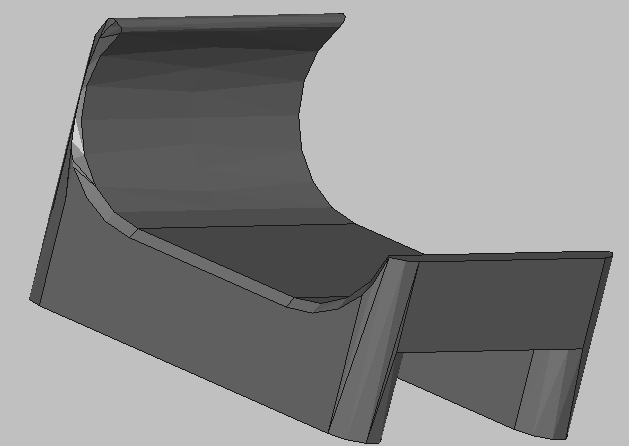
\includegraphics[width=.85\textwidth]{sec2/images/3DAnbaukomponenten/Konstruktionsbilder/AkkuHalterungKonstruktion} 
\centering
\captionsetup{width=.9\textwidth}
\caption[Konstruktionsbild der Akku-Halterung]{Konstruktionsbild der Akku-Halterung mit Kabeldurchführung}\centering
\label{fig:AkkuHalterungKonstruktion}
\end{figure}
\end{minipage}
\begin{minipage}[b]{0.45\textwidth}
\begin{figure}[H] %H für Positionierung hier
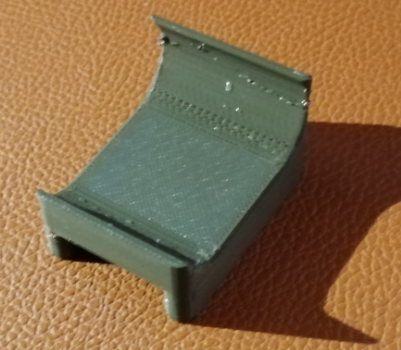
\includegraphics[width=.85\textwidth]{sec2/images/3DAnbaukomponenten/Druckbilder/AkkuHalterungDruck} 
\centering
\captionsetup{width=.9\textwidth}
\caption[Gedruckte Akku-Halterung]{Gedruckte Akku-Halterung}\centering
\label{fig:AkkuHalterungDruck}
\end{figure}
\end{minipage}
\vspace{4mm}

Während die Akku-Halterung den Akku vor dem nach vorne und hinten rutschen schützt, tragen kleine Aussparungen an den Innenseiten der Seitenschweller zur Sicherung des Akkus zu beiden Seiten bei (Konstruktionszeichnung in Abbildung \ref{fig:SeitenschwellerKonstruktion}). Sie werden mit je drei Schrauben an der Grundplatte des Fahrzeugs befestigt. Die fertig gedruckten Seitenschweller sind in Abbildung \ref{fig:SeitenschwellerDruck} abgebildet.

\begin{minipage}[t]{0.47\textwidth}
\centering
\begin{figure}[H] %H für Positionierung hier
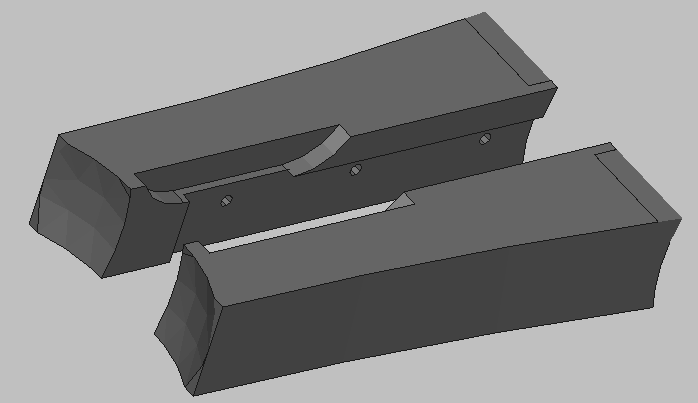
\includegraphics[width=.85\textwidth]{sec2/images/3DAnbaukomponenten/Konstruktionsbilder/SeitenschwellerKonstruktion} 
\centering
\captionsetup{width=.9\textwidth}
\caption[Konstruktionsbild der Seitenschweller]{Konstruktionsbild der Seitenschweller, welche auch als Sicherung des Akkus zu den Seiten dienen}
\centering
\label{fig:SeitenschwellerKonstruktion}
\end{figure}
\end{minipage}
\begin{minipage}[t]{0.47\textwidth}
\begin{figure}[H] %H für Positionierung hier
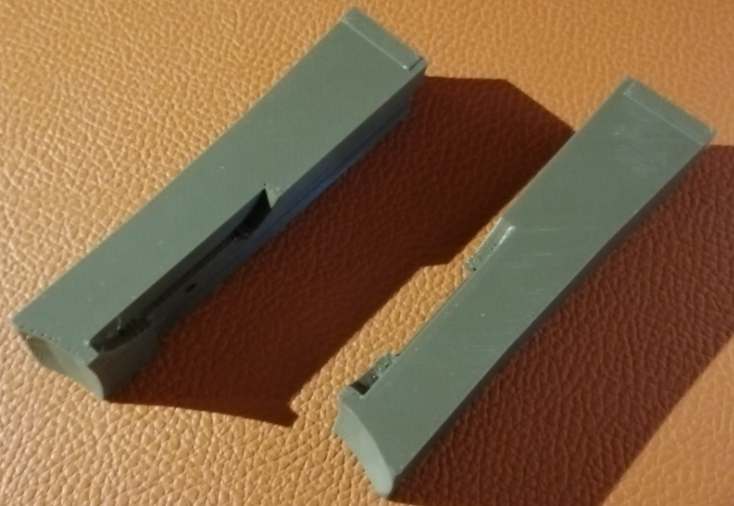
\includegraphics[width=.85\textwidth]{sec2/images/3DAnbaukomponenten/Druckbilder/SeitenschwellerDruck} 
\centering
\captionsetup{width=.95\textwidth}
\caption[Gedruckte Seitenschweller]{Gedruckte Seitenschweller}\centering
\label{fig:SeitenschwellerDruck}
\end{figure}
\end{minipage}
\vspace{4mm}

In Abbildung \ref{fig:SchwellerAkkuHalterungMontage} sind die zum Fixieren des Akkus notwendigen Teile, die Seitenschweller und die Akku-Halterung, am Fahrzeug fertig montiert, abgebildet. Der Akku wird quer zur Fahrtrichtung eingesetzt. So bleibt hinter dem Akku noch Platz für eine Verteilerplatine, an der die elektrischen Anschlüsse der verschiedenen Fahrzeugkomponenten angesteckt werden können.

\begin{figure}[H] %H für Positionierung hier
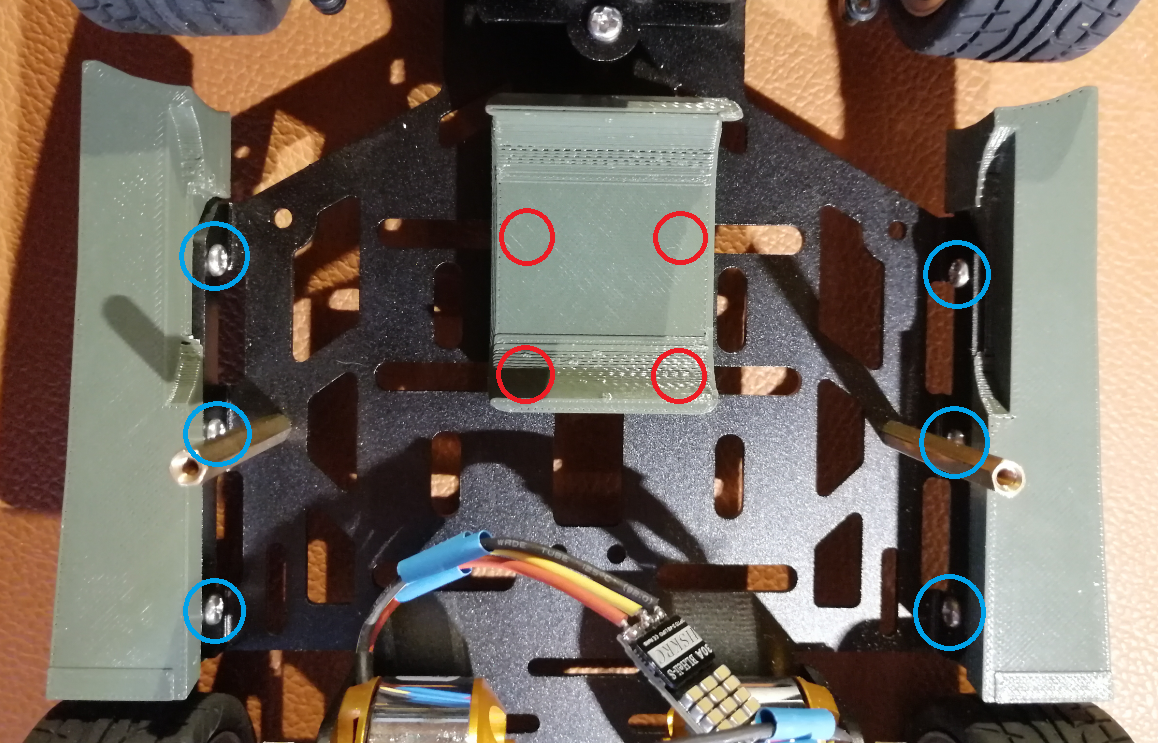
\includegraphics[width=.7\textwidth]{sec2/images/3DAnbaukomponenten/Montagebilder/SchwellerAkkuHalterungMontage} 
\centering
\captionsetup{width=.95\textwidth}
\caption[Montierte Akku-Halterung und Seitenschweller]{Montierte Akku-Halterung und Seitenschweller; Befestigungsschrauben der Seitenschweller in blau und Befestigungsschrauben der Akkuhalterung in rot (von unten, nicht sichtbar)}\centering
\label{fig:SchwellerAkkuHalterungMontage}
\end{figure}

\newpage

\subsubsection{Halterung der Controllerplatine und des Bedienungsboards}\label{Sec2Sub2SubSub3}

Die Controllerplatine wird auf der oberen Fahrzeugplattform befestigt. Dafür wird eine Controller-Halterung benötigt (Konstruktionsbild siehe Abbildung \ref{fig:ControllerHalterungKonstruktion}). Oberhalb des Controllers findet das Display mit Bedientaster und Drehencoder für die Menüsteuerung Platz (Bedienungsboard). Zusätzlich zur Halterung der Platine (Konstruktionsbild siehe Abbildung \ref{fig:PlatinenHalterungKonstruktion}) ist eine Abdeckung notwendig (Konstruktionsbild siehe Abbildung \ref{fig:DisplayAbdeckungKonstruktion}).

\begin{figure}[H] %H für Positionierung hier
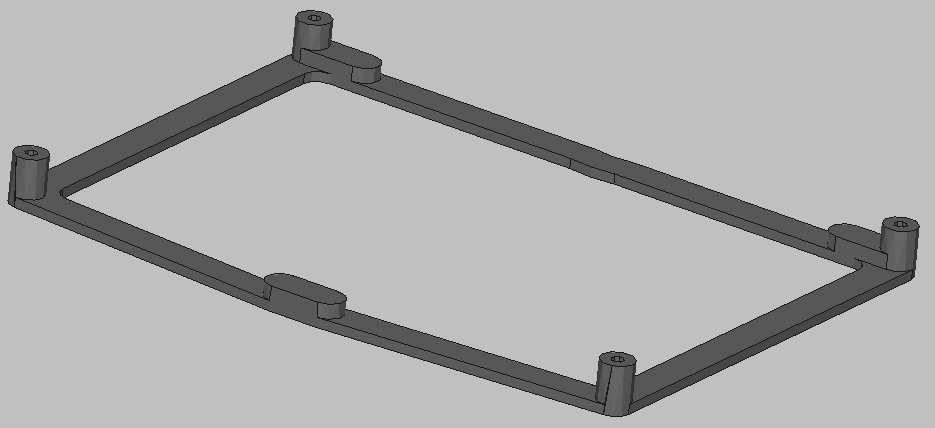
\includegraphics[width=.85\textwidth]{sec2/images/3DAnbaukomponenten/Konstruktionsbilder/ControllerHalterungKonstruktion} 
\centering
\captionsetup{width=.9\textwidth}
\caption[Konstruktionsbild der Controller-Halterung]{Konstruktionsbild der Controller-Halterung}
\centering
\label{fig:ControllerHalterungKonstruktion}
\end{figure}

\hspace{-3mm}
\begin{minipage}[t]{0.47\textwidth}
\vspace{-6mm}
\begin{figure}[H] %H für Positionierung hier
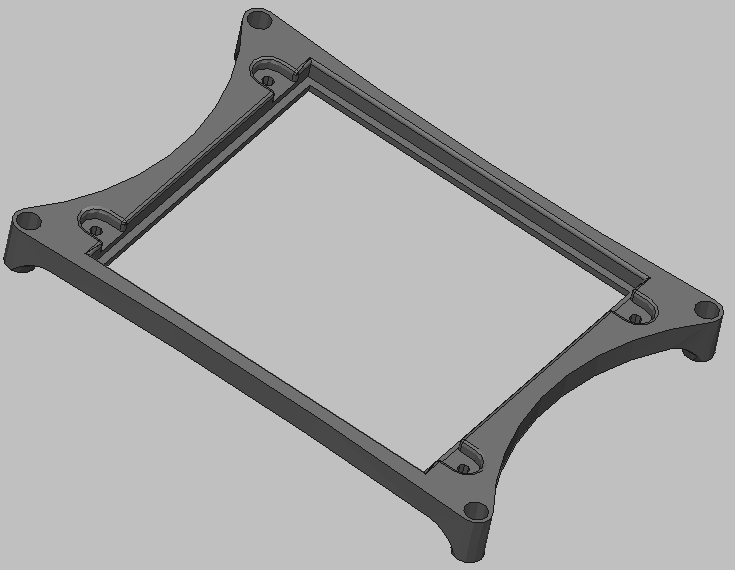
\includegraphics[width=.85\textwidth]{sec2/images/3DAnbaukomponenten/Konstruktionsbilder/PlatinenHalterungKonstruktion} 
\centering
\captionsetup{width=.9\textwidth}	
\caption[Konstruktionsbild der Platinen-Halterung des Bedienungsboards]{Konstruktionsbild der Platinen-Halterung des Bedienungsboards}
\centering
\label{fig:PlatinenHalterungKonstruktion}
\end{figure}
\end{minipage}
\begin{minipage}[t]{0.47\textwidth}
\vspace{-6mm}
\begin{figure}[H] %H für Positionierung hier
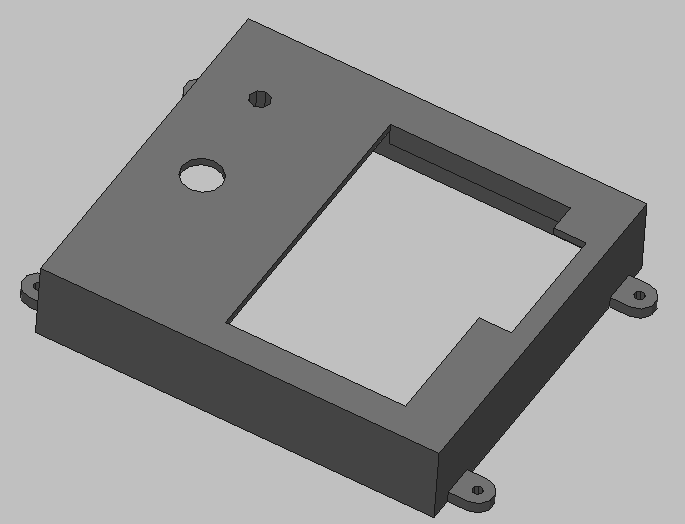
\includegraphics[width=.85\textwidth]{sec2/images/3DAnbaukomponenten/Konstruktionsbilder/DisplayAbdeckungKonstruktion} 
\centering
\captionsetup{width=.9\textwidth}
\caption[Konstruktionsbild der Abdeckung des Bedienungsboards]{Konstruktionsbild der Abdeckung des Bedienungsboards}
\centering
\label{fig:DisplayAbdeckungKonstruktion}
\end{figure}
\end{minipage}
\vspace{4mm}


\begin{minipage}[t]{0.54\textwidth}
\indent Zum Bedienen des Drucktasters auf der Platine wird eine Verlängerung benötigt, damit der Knopf außerhalb der Abdeckung betätigt werden kann (Konstruktionszeichnung siehe Abbildung \ref{fig:DruckTasterKonstruktion}). In den Abbildungen \ref{fig:ControllerHalterungDruck} bis \ref{fig:DruckTasterDruck} sind die fertig gedruckten Teile, die Controller-Halterung, die Platinen-Halterung und die Abdeckung, abgebildet.
\end{minipage}
\begin{minipage}[t]{0.4\textwidth}
\vspace{-7mm}
\begin{figure}[H] %H für Positionierung hier
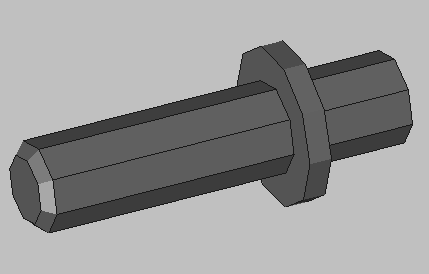
\includegraphics[width=.7\textwidth]{sec2/images/3DAnbaukomponenten/Konstruktionsbilder/DruckTasterKonstruktion} 
\centering
\captionsetup{width=.9\textwidth}
\caption[Konstruktionsbild des Drucktasters]{Konstruktionsbild des Drucktasters}
\centering
\label{fig:DruckTasterKonstruktion}
\end{figure}
\end{minipage}

\begin{minipage}[b]{0.54\textwidth}
\centering
\vspace{-6mm}
\begin{figure}[H] %H für Positionierung hier
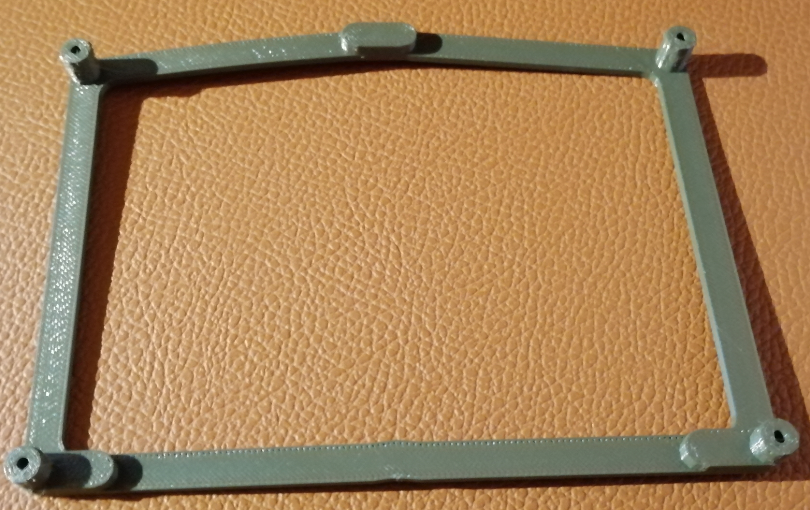
\includegraphics[width=.85\textwidth]{sec2/images/3DAnbaukomponenten/Druckbilder/ControllerHalterungDruck} 
\centering
\captionsetup{width=.95\textwidth}
\caption[Gedruckte Controller-Halterung]{Gedruckte Controller-Halterung}\centering
\label{fig:ControllerHalterungDruck}
\end{figure}
\end{minipage}
\begin{minipage}[b]{0.36\textwidth}
\vspace{-6mm}
\begin{figure}[H] %H für Positionierung hier
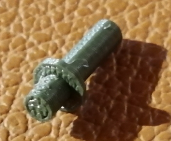
\includegraphics[width=.8\textwidth]{sec2/images/3DAnbaukomponenten/Druckbilder/DruckTasterDruck} 
\centering
\captionsetup{width=.95\textwidth}
\caption[Gedruckte Drucktaster-Verlängerung]{Gedruckte Drucktaster-Verlängerung}
\centering
\label{fig:DruckTasterDruck}
\end{figure}
\end{minipage}


\begin{minipage}[b]{0.46\textwidth}
\centering
\begin{figure}[H] %H für Positionierung hier
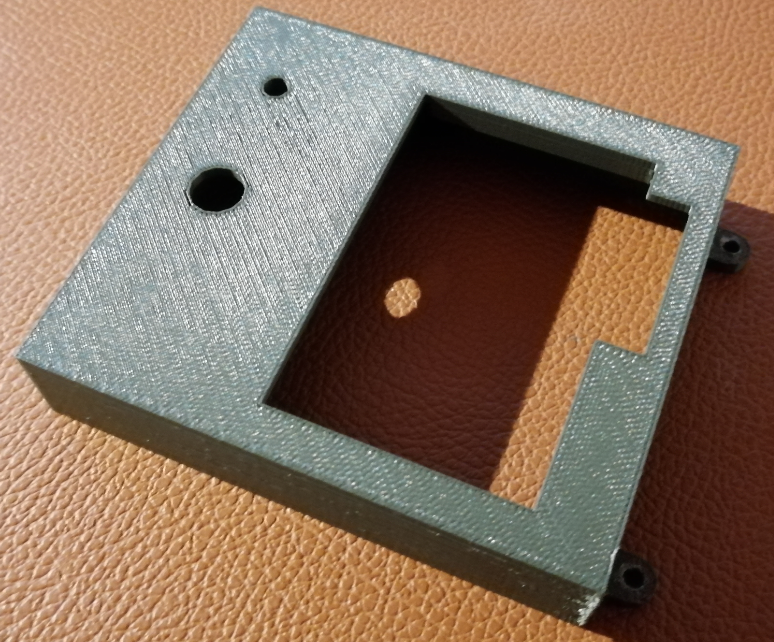
\includegraphics[width=.9\textwidth]{sec2/images/3DAnbaukomponenten/Druckbilder/DisplayAbdeckungDruck} 
\centering
\captionsetup{width=.95\textwidth}
\caption[Gedruckte Platinen-Abdeckung des Bedienungsboards]{Gedruckte Platinen-Abdeckung des Bedienungsboards}\centering
\label{fig:DisplayAbdeckungDruck}
\end{figure}
\end{minipage}
\begin{minipage}[b]{0.46\textwidth}
\begin{figure}[H] %H für Positionierung hier
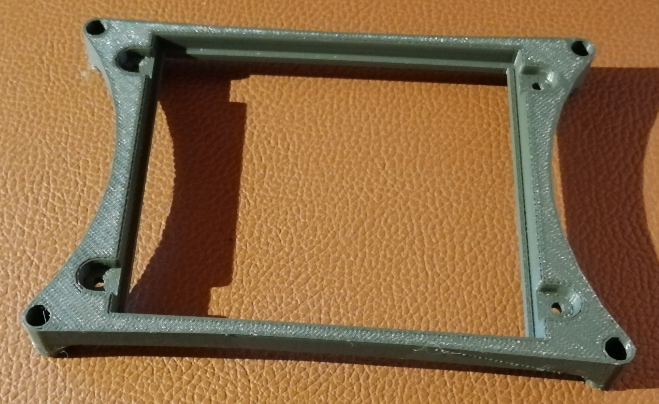
\includegraphics[width=.9\textwidth]{sec2/images/3DAnbaukomponenten/Druckbilder/PlatinenHalterungDruck} 
\centering
\captionsetup{width=.95\textwidth}
\caption[Gedruckte Platinen-Halterung für das Bedienungsboard]{Gedruckte Platinen-Halterung für das Bedienungsboard}\centering
\label{fig:PlatinenHalterungDruck}
\end{figure}
\end{minipage}
\vspace{4mm}

Die Montage der Teile erfolgt, wie bereits erwähnt, auf der oberen Fahrzeugebene. In den Abbildungen \ref{fig:ControllerMontage} und \ref{fig:AbdeckungMontage} sind die fertig montierten Komponenten für die Befestigung des Controllers und die der Platine für die Fahrzeugbedienung abgebildet. Damit für die Komponenten auf der Controllerplatine ausreichend Platz ist, wird die Platinen-Halterung des Bedienungsboards über Abstandshalterungen montiert. Die Befestigungsschrauben für den Controller sind in den Abbildungen mit roten Kreisen, die der Platinenhalterung mit blauen Kreisen und die der Abdeckung mit gelben Kreisen hervorgehoben.

\begin{figure}[H] %H für Positionierung hier
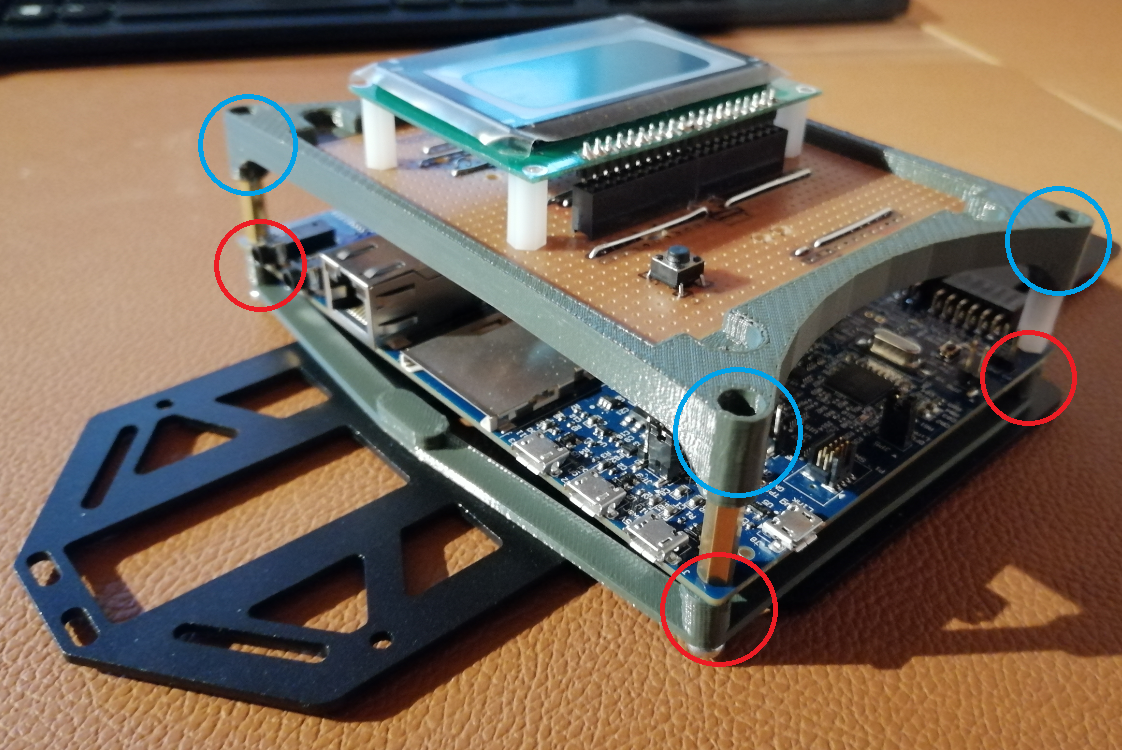
\includegraphics[width=.8\textwidth]{sec2/images/3DAnbaukomponenten/Montagebilder/ControllerMontage} 
\centering
\captionsetup{width=.95\textwidth}
\caption[Fertig montierte Controller- und Bedienungsboard-Halterung]{Fertig montierte Controller- und Bedienungsboard-Halterung; Befestigungsschrauben des Controllers in rot, Befestigung der Platinen-Halterung in blau}\centering
\label{fig:ControllerMontage}
\end{figure}

\begin{figure}[H] %H für Positionierung hier
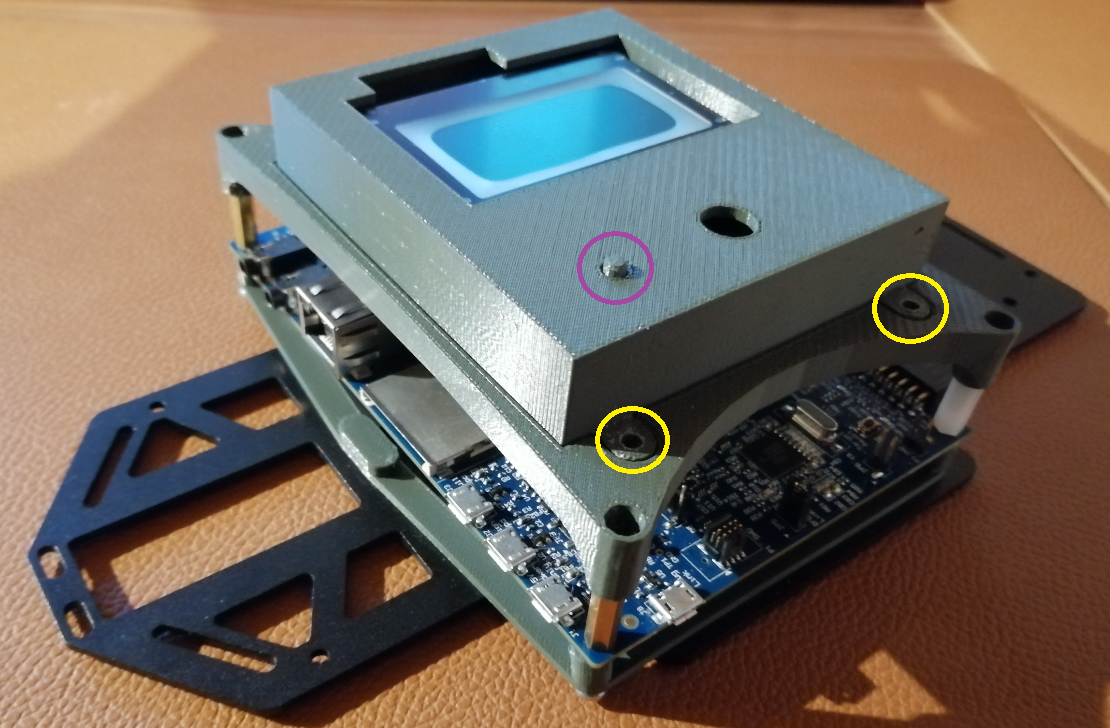
\includegraphics[width=.8\textwidth]{sec2/images/3DAnbaukomponenten/Montagebilder/AbdeckungMontage} 
\centering
\captionsetup{width=.95\textwidth}
\caption[Fertig montierte Controller- und Bedienungsboard-Halterung mit Abdeckung]{Fertig montierte Controller- und Bedienungsboard-Halterung mit Abdeckun; Befestigungsschrauben der Abdeckung in gelb, Taster in violett}\centering
\label{fig:AbdeckungMontage}
\end{figure}

\newpage

\subsubsection{Halterung für die Motorcontroller}\label{Sec2Sub2SubSub4}
%*************************************************************************
%Bilder mit montierten Motorcontroller-Halterungen und Text dazu verfassen
%*************************************************************************

Die Motorcontroller, die vor die BLDC-Motoren geschaltet sind, werden auf der Grundplatte befestigt. Mit zwei dreiecksförmigen Halterungen werden die Motorcontroller an jeweils drei stellen an der Grundplatte angeschraubt. Die Konstruktionszeichnung einer solchen Motorcontroller-Halterung ist in Abbildung \ref{fig:MotorcontrollerHalterungKonstruktion} und das Druckergebnis in Abbildung \ref{fig:MotorcontrollerHalterungDruck} einsehbar.

\begin{minipage}[b]{0.47\textwidth}
\centering
\begin{figure}[H] %H für Positionierung hier
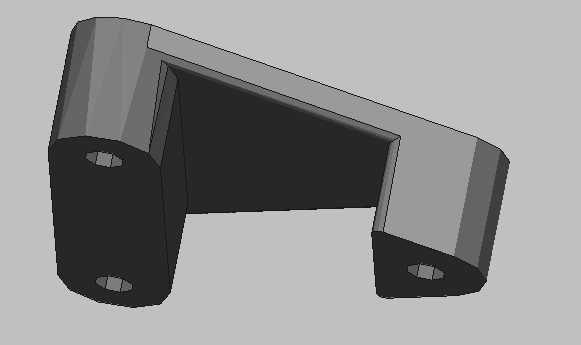
\includegraphics[width=.8\textwidth]{sec2/images/3DAnbaukomponenten/Konstruktionsbilder/MotorcontrollerHalterungKonstruktion} 
\centering
\captionsetup{width=.9\textwidth}
\caption[Konstruktionsbild einer Motorcontroller-Halterung]{Konstruktionsbild einer Motorcontroller-Halterung}
\centering
\label{fig:MotorcontrollerHalterungKonstruktion}
\end{figure}
\end{minipage}
\begin{minipage}[b]{0.47\textwidth}
\begin{figure}[H] %H für Positionierung hier
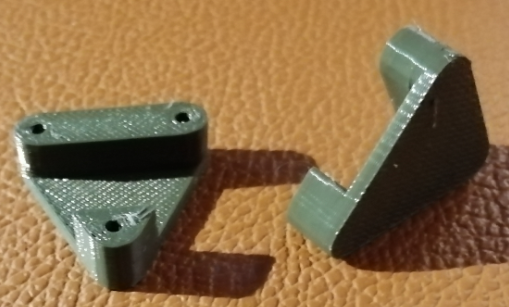
\includegraphics[width=.8\textwidth]{sec2/images/3DAnbaukomponenten/Druckbilder/MotorcontrollerHalterungDruck} 
\centering
\captionsetup{width=.95\textwidth}
\caption[Gedruckte Motorcontroller-Halterungen]{Fertig Gedruckte Motorcontroller-Halterungen}
\centering
\label{fig:MotorcontrollerHalterungDruck}
\end{figure}
\end{minipage}
\vspace{4mm}

Abbildung \ref{fig:MotorcontrollerHalterungMontage} zeigt die auf der Grundplatte moniterten Motorcontroller-Halterungen. Die Controller sind am Boden fixiert und durch den transparenten Schrumpfschlauch vor Kurzschlüssen über die metallische Grundplatte geschützt.

\begin{figure}[H] %H für Positionierung hier
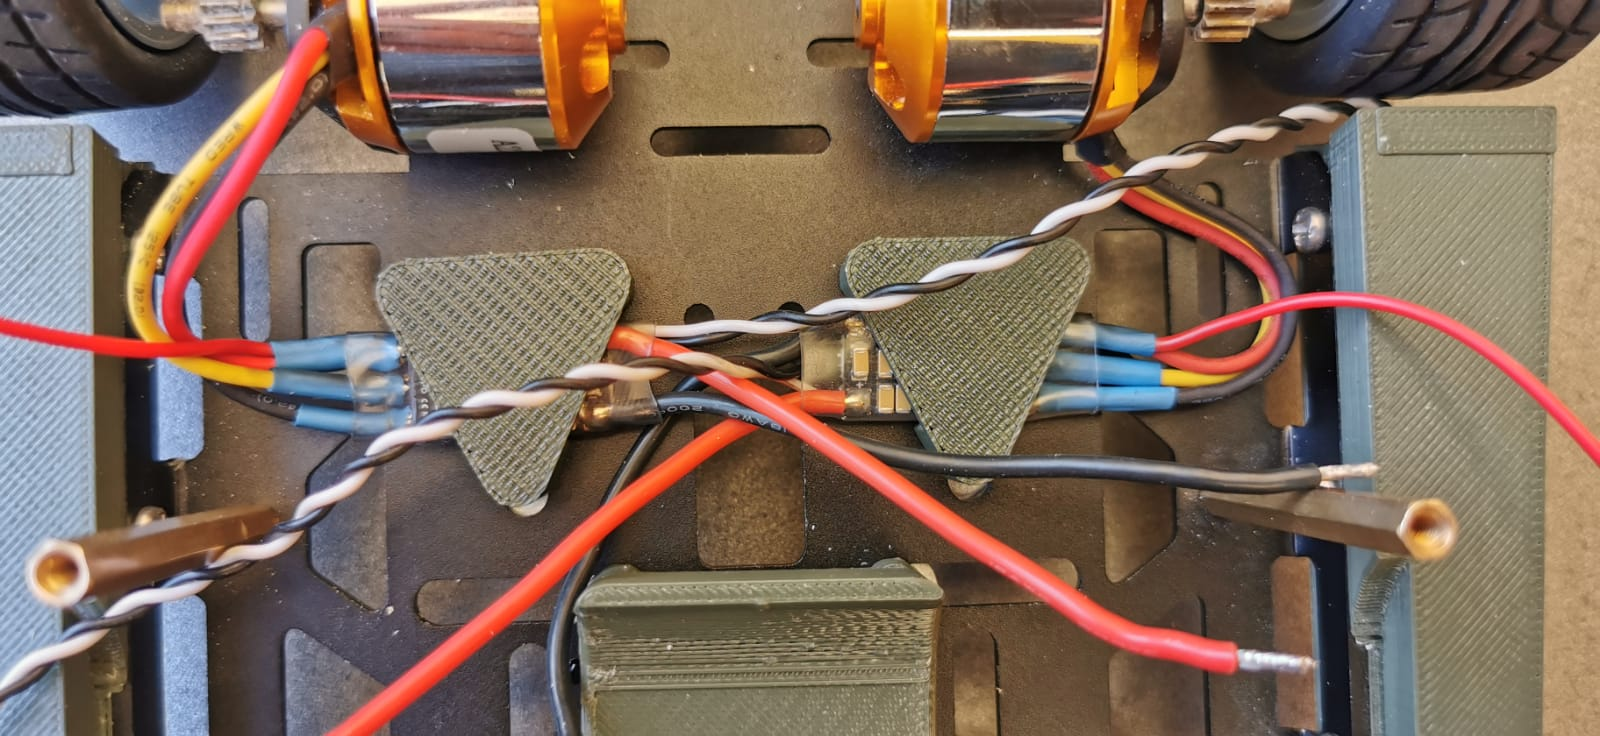
\includegraphics[width=.85\textwidth]{sec2/images/3DAnbaukomponenten/Montagebilder/MotorcontrollerHalterungMontage} 
\centering
\captionsetup{width=.95\textwidth}
\caption[Die auf der Grundplatte montierten Motorcontroller]{Die auf der Grundplatte montierten Motorcontroller}
\centering
\label{fig:MotorcontrollerHalterungMontage}
\end{figure}

\newpage

\subsubsection{Einfache Platinenhalterungen}\label{Sec2Sub2SubSub5}

Für die Befestigung der Verteiler-Platine auf der unteren Ebene wird eine Halterung benötigt. Mit vier einfachen Halterungen (Konstruktionsbild siehe Abbildung \ref{fig:PlatinenHalterungenKonstruktion}) kann die Lochrasterplatine an vier Stellen mit etwas Abstand zur Grundplatte auf dieser befestigt werden. Die fertig gedruckten Platinen-Halterungen sind in Abbildung \ref{fig:PlatinenHalterungenDruck} abgebildet.

\begin{minipage}[b]{0.4\textwidth}
\centering
\begin{figure}[H] %H für Positionierung hier
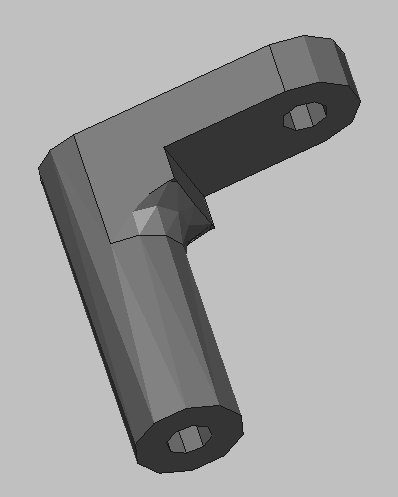
\includegraphics[width=.5\textwidth]{sec2/images/3DAnbaukomponenten/Konstruktionsbilder/PlatinenHalterungenKonstruktion} 
\centering
\captionsetup{width=.9\textwidth}
\caption[Konstruktionsbild einer einfachen Platinenhalterung]{Konstruktionsbild einer einfachen Platinenhalterung}
\centering
\label{fig:PlatinenHalterungenKonstruktion}
\end{figure}
\end{minipage}
\begin{minipage}[b]{0.54\textwidth}
\begin{figure}[H] %H für Positionierung hier
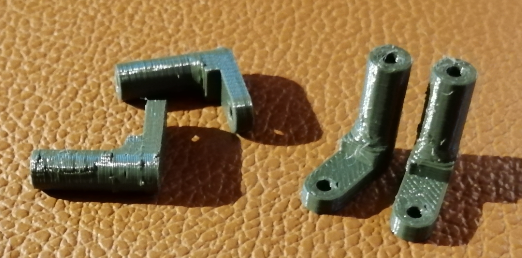
\includegraphics[width=.9\textwidth]{sec2/images/3DAnbaukomponenten/Druckbilder/PlatinenHalterungenDruck} 
\centering
\captionsetup{width=.95\textwidth}
\caption[Gedruckte Platinenhalterungen]{Gedruckte Platinenhalterungen}
\centering
\label{fig:PlatinenHalterungenDruck}
\end{figure}
\end{minipage}
\vspace{8mm}

In Abbildung \ref{fig:PlatinenHalterungenMontage} ist die fertig montierte Verteiler-Platine sichtbar. Sie ist mit vier einfachen Platinen-Halterungen an der Grundplatte des Fahrzeugs montiert. Der aufgrund der Halterungen resultierende Abstand zur Grundplatte ermöglicht die Montage der Motorcontroller-Halterungen unter der Verteiler-Platine.

\begin{figure}[H] %H für Positionierung hier

\includegraphics[width=.70\textwidth]{sec2/images/3DAnbaukomponenten/Montagebilder/PlatinenHalterungenMontage} 
\centering
\captionsetup{width=.8\textwidth}
\caption[Mit den Platinenhalterungen montierte Versorgungsspannungs-Verteilerplatine ]{Mit den einfachen Platinenhalterungen montierte Verteilerplatine für die Versorgungsspannung}
\centering
\label{fig:PlatinenHalterungenMontage}
\end{figure}

\subsubsection{Kamerahalterung}\label{Sec2Sub2SubSub6}

Die Kamera soll sich bei Kollisionen nicht in ihrer Position verstellen können. Deshalb wird eine eigens dafür konstruierte Halterung gedruckt. Im Gegensatz zu den bisherigen 3D-Druckteilen sind die Kamerahalterung und die Antriebsabdeckung (siehe Kapitel \ref{Sec2Sub2SubSub7}) selbst konstruiert und nicht vom Vorgänger übernommen. Die Konstruktionsbilder der beiden Einzelteile der Kamerahalterung sind in den Abbildungen \ref{fig:KameraHalterungKonstruktion02} und \ref{fig:KameraHalterungKonstruktion01} einsehbar. Die ineinandergreifenden Zacken garantieren dabei eine stabile Kameraposition.

\begin{minipage}[b]{0.44\textwidth}
\centering
\begin{figure}[H] %H für Positionierung hier
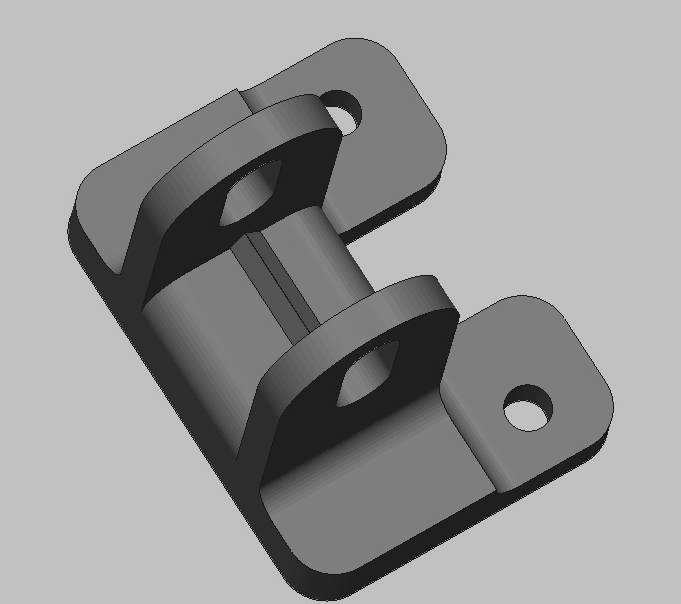
\includegraphics[width=.8\textwidth]{sec2/images/3DAnbaukomponenten/Konstruktionsbilder/KameraHalterungKonstruktion02} 
\centering
\captionsetup{width=.9\textwidth}
\caption[Kameramontage-Komponente der Kamera-Halterung]{Kameramontage-Komponente der Kamera-Halterung}
\centering
\label{fig:KameraHalterungKonstruktion02}
\end{figure}
\end{minipage}
\begin{minipage}[b]{0.5\textwidth}
\begin{figure}[H] %H für Positionierung hier
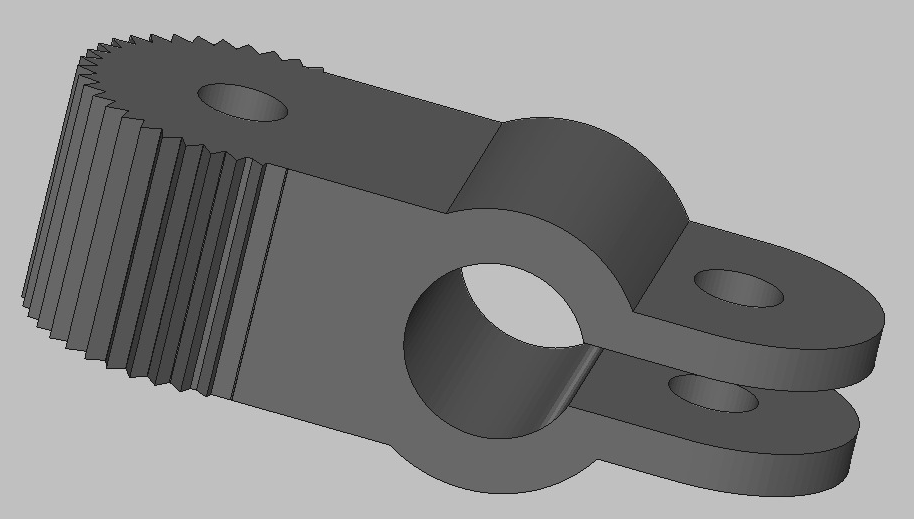
\includegraphics[width=.8\textwidth]{sec2/images/3DAnbaukomponenten/Konstruktionsbilder/KameraHalterungKonstruktion01} 
\centering
\captionsetup{width=.9\textwidth}
\caption[Stangenmontage-Komponente der Kamera-Halterung]{Stangenmontage-Komponente der Kamera-Halterung}
\centering
\label{fig:KameraHalterungKonstruktion01}
\end{figure}
\end{minipage}
\vspace{2mm}

Schon bei der Konstruktion zeichnet sich ein potentielles Problem für den Druck der Teile ab. Die Verzahnung ist sehr fein gewählt, um die Kamera auch genau einstellen zu können. Für einen 3D-Drucker kann das bedeuten, dass dieser an seine Grenzen in der Genauigkeit der Fertigung kommt. Die Sorge, dass der verwendete 3D-Drucker, welcher \ac{ABS} verwendet, die Verzahnung nicht fein genug fertigen kann, ist zum Teil begründet, da von je zwei gedruckten Teilen eines jeder Komponente von ungenügender Genauigkeit ist. Die beiden in ausreichender Qualität gefertigten Teile sind in Abbildung \ref{fig:KameraHalterungMontage} abgebildet. Mit der Erwartung, genauere Ergebnisse zu erzielen, müsste auf den \ac{SLA} der Fakultät Maschinenbau zurückgegriffen werden. In diesem Fall ist das allerdings nicht notwendig.\vspace{11pt}

Bei der Montage taucht allerdings ein anderes, unerwartetes Problem auf. Bei der Konstruktion der Teile wurde an einer Stelle entweder ein falsches Maß aufgenommen oder das Maß falsch in die CAD-Zeichnung eingegeben. Die betreffende Stelle ist die Freifläche zwischen den beiden Befestigungsstellen der Kamera, welche um etwa 1,5mm zu kurz geraten ist. Nach einer Anpassung mit einer Säge sind die Teile ohne Probleme verwendbar und die Komponente muss nicht abermals gedruckt werden. Zur Vermeidung dieser Anpassung für Nachfolgemodelle des Fahrzeugs ist die Konstruktionszeichnung angepasst.

\begin{figure}[H] %H für Positionierung hier
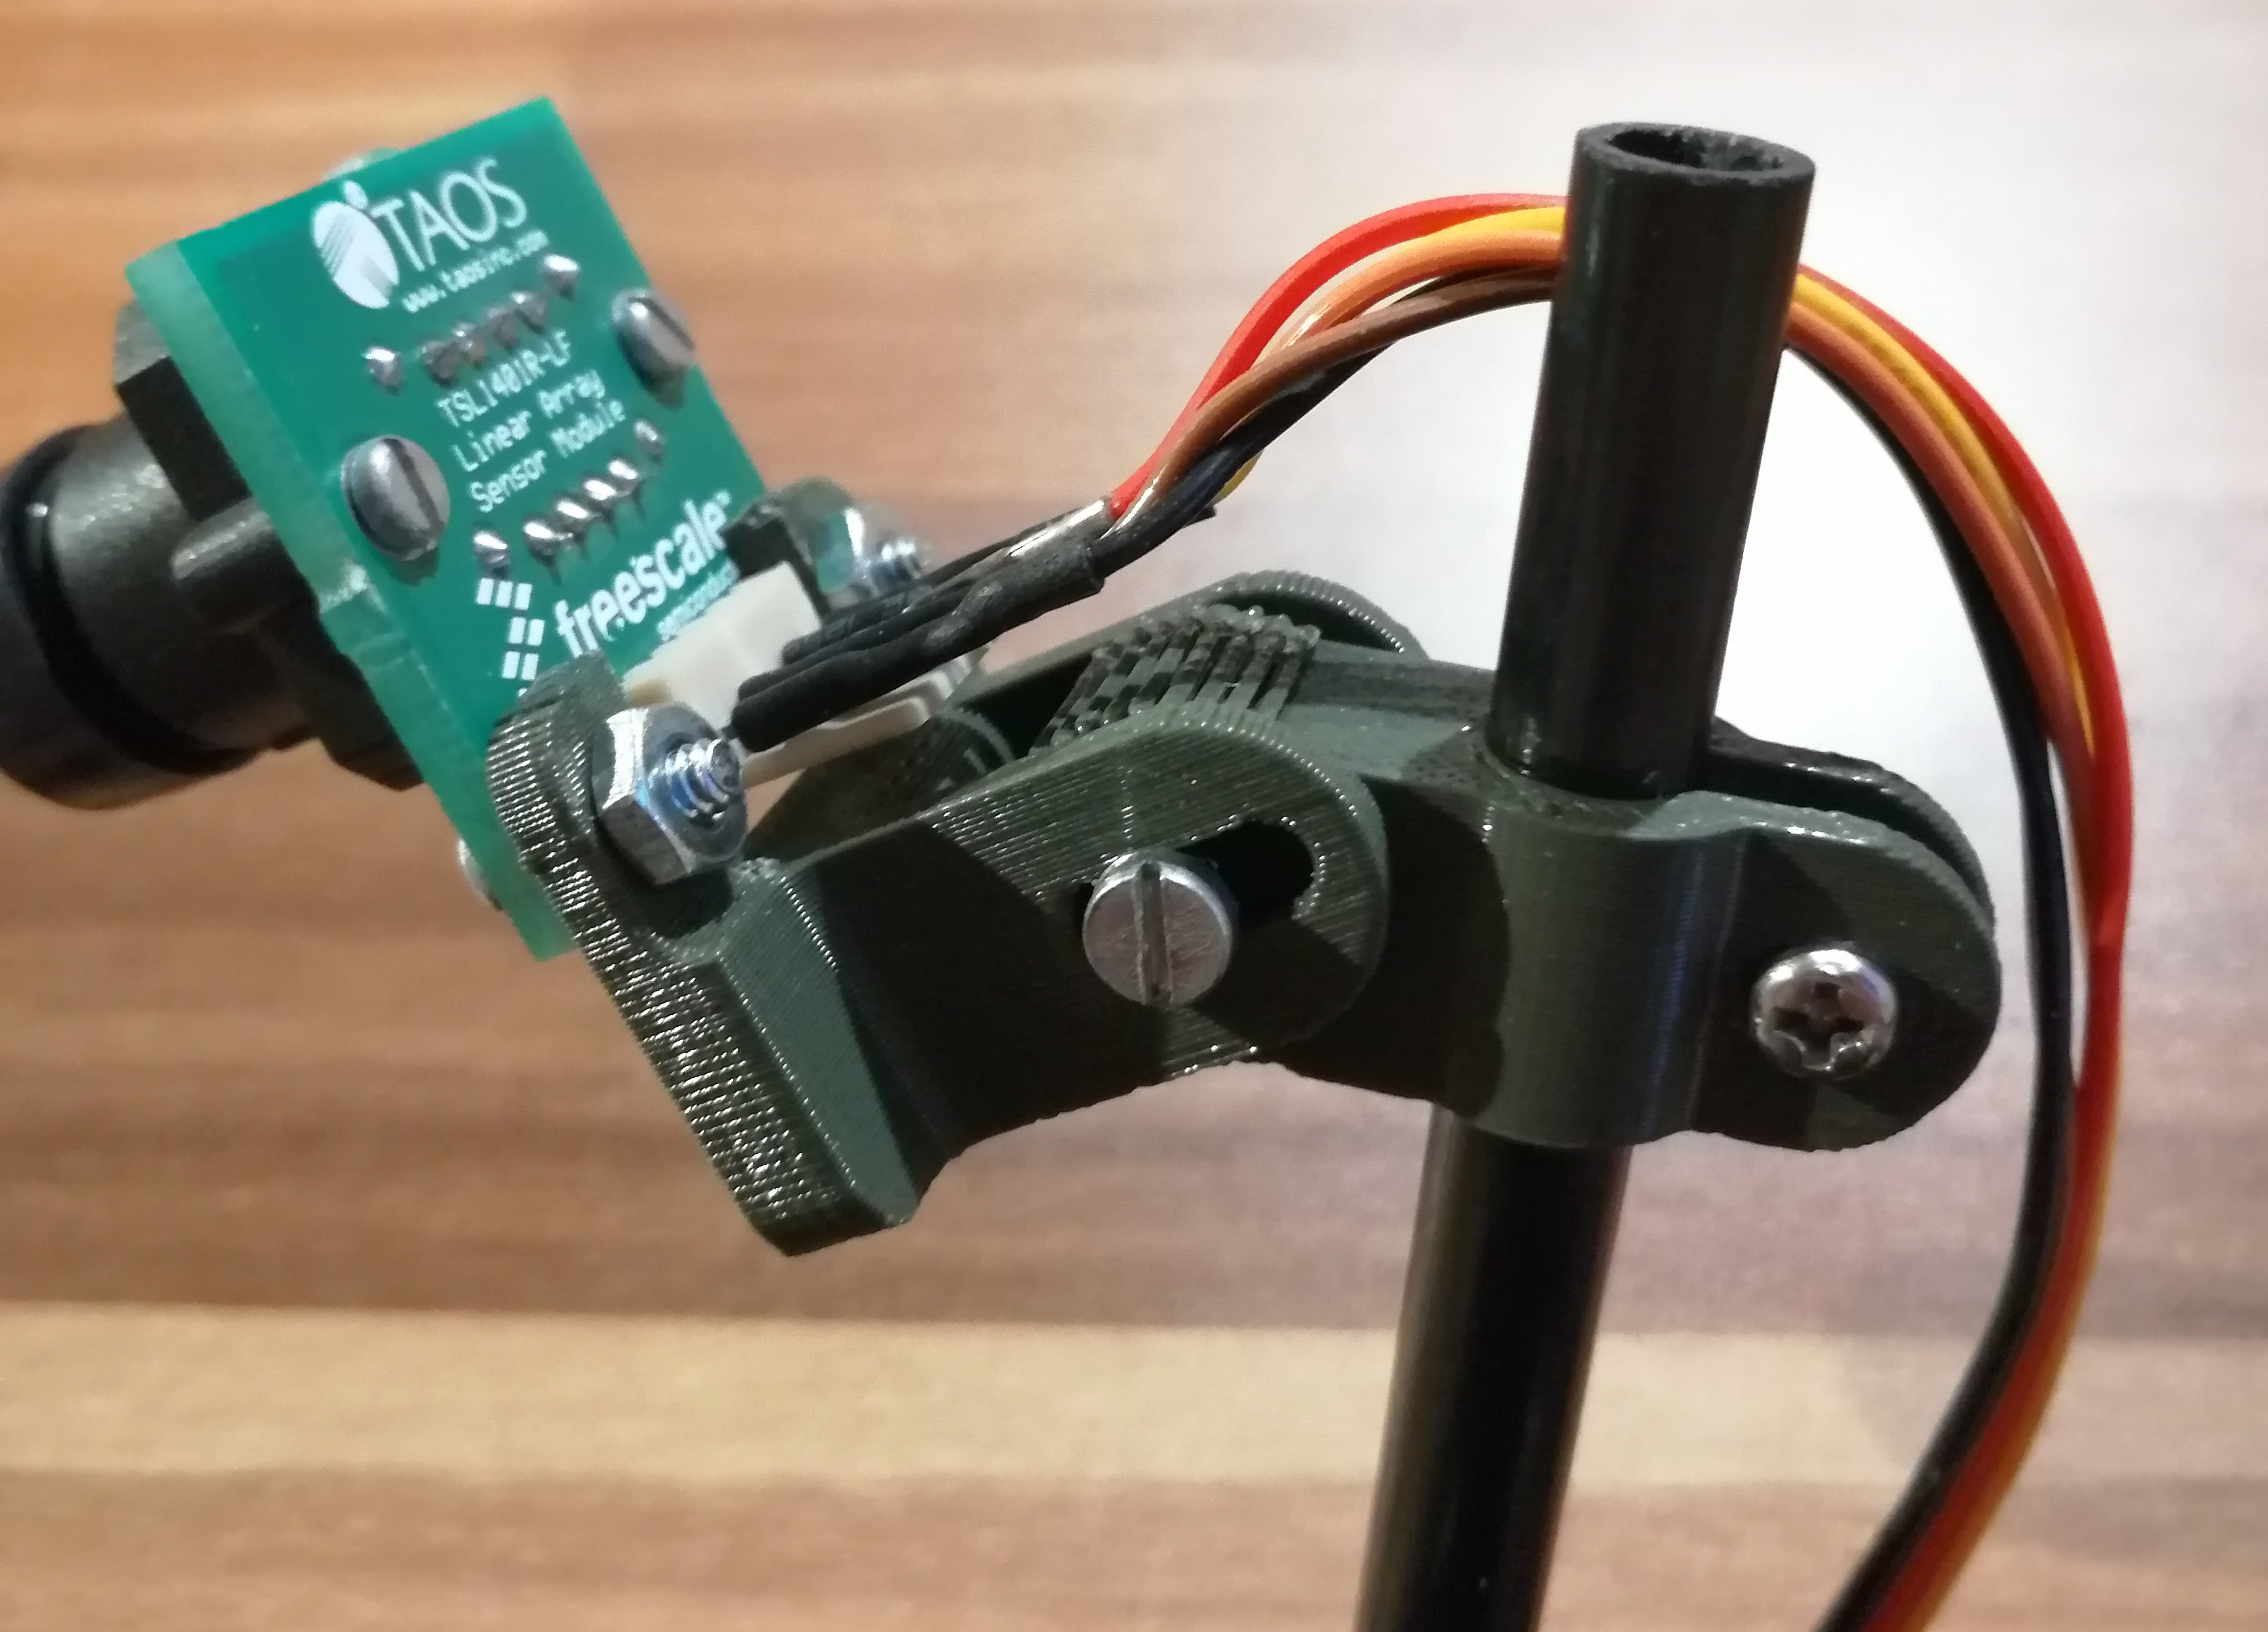
\includegraphics[width=.70\textwidth]{sec2/images/3DAnbaukomponenten/Montagebilder/KameraHalterungMontage} 
\centering
\captionsetup{width=.9\textwidth}
\caption[Fertig montierte Kamera mit Kamerahalterung]{Fertig montierte Kamera mit Kamerahalterung}
\centering
\label{fig:KameraHalterungMontage}
\end{figure}


\subsubsection{Antriebs-Abdeckung}\label{Sec2Sub2SubSub7}

Da die Kabel der Komponenten auf der Grundplatte, welche auf der oberen Ebene angesteckt werden, nicht mittig zwischen den beiden Antrieben auf die obere Ebene durchgeführt werden können, weil dort der Sockel der Kamerastange Platz findet, müssen die Kabel direkt über den Antrieben durchgeführt werden. Das führt allerdings dazu, dass sich die Kabelisolierungen durch die Reibung an den sich drehenden Antrieben über die Zeit abtragen können. Aus diesem Grund wird eine Antriebs-Abdeckung benötigt.Das Konstruktionsbild und das der fertig gedruckten Antriebsabdeckung sind in den Abbildungen  \ref{fig:KonstruktionAntriebsabdeckung} und \ref{fig:DruckAntriebsabdeckung} einsehbar. Die fertig montierte Antriebsabdeckung ist in Abbildung \ref{fig:MontageAntriebsabdeckung} abgebildet.

\begin{minipage}[b]{0.49\textwidth}
\centering
\begin{figure}[H] %H für Positionierung hier
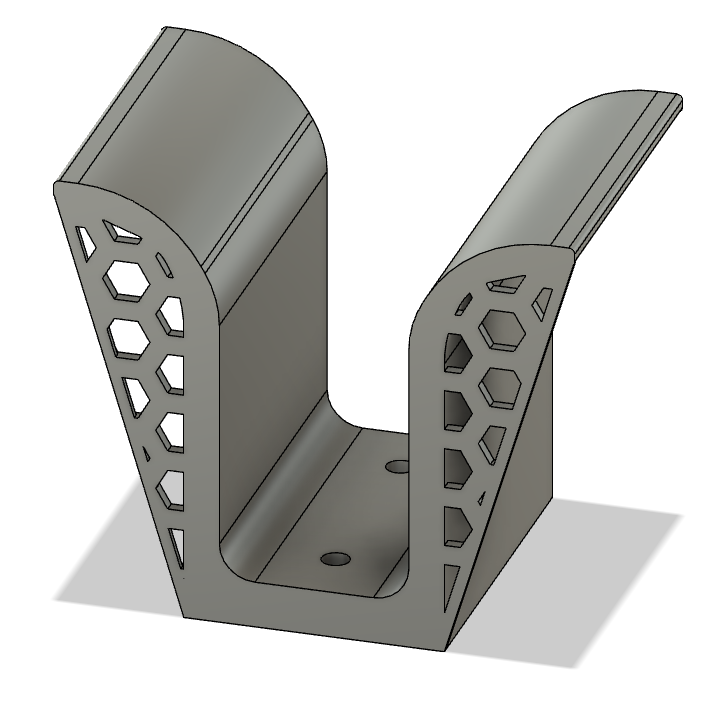
\includegraphics[width=.8\textwidth]{sec2/images/3DAnbaukomponenten/Konstruktionsbilder/AntriebsabdeckungKonstruktion} 
\centering
\captionsetup{width=.9\textwidth}
\caption[Konstruktionsbild der Antriebsabdeckung]{Konstruktionsbild der Antriebsabdeckung}
\centering
\label{fig:KonstruktionAntriebsabdeckung}
\end{figure}
\end{minipage}
\begin{minipage}[b]{0.49\textwidth}
\begin{figure}[H] %H für Positionierung hier
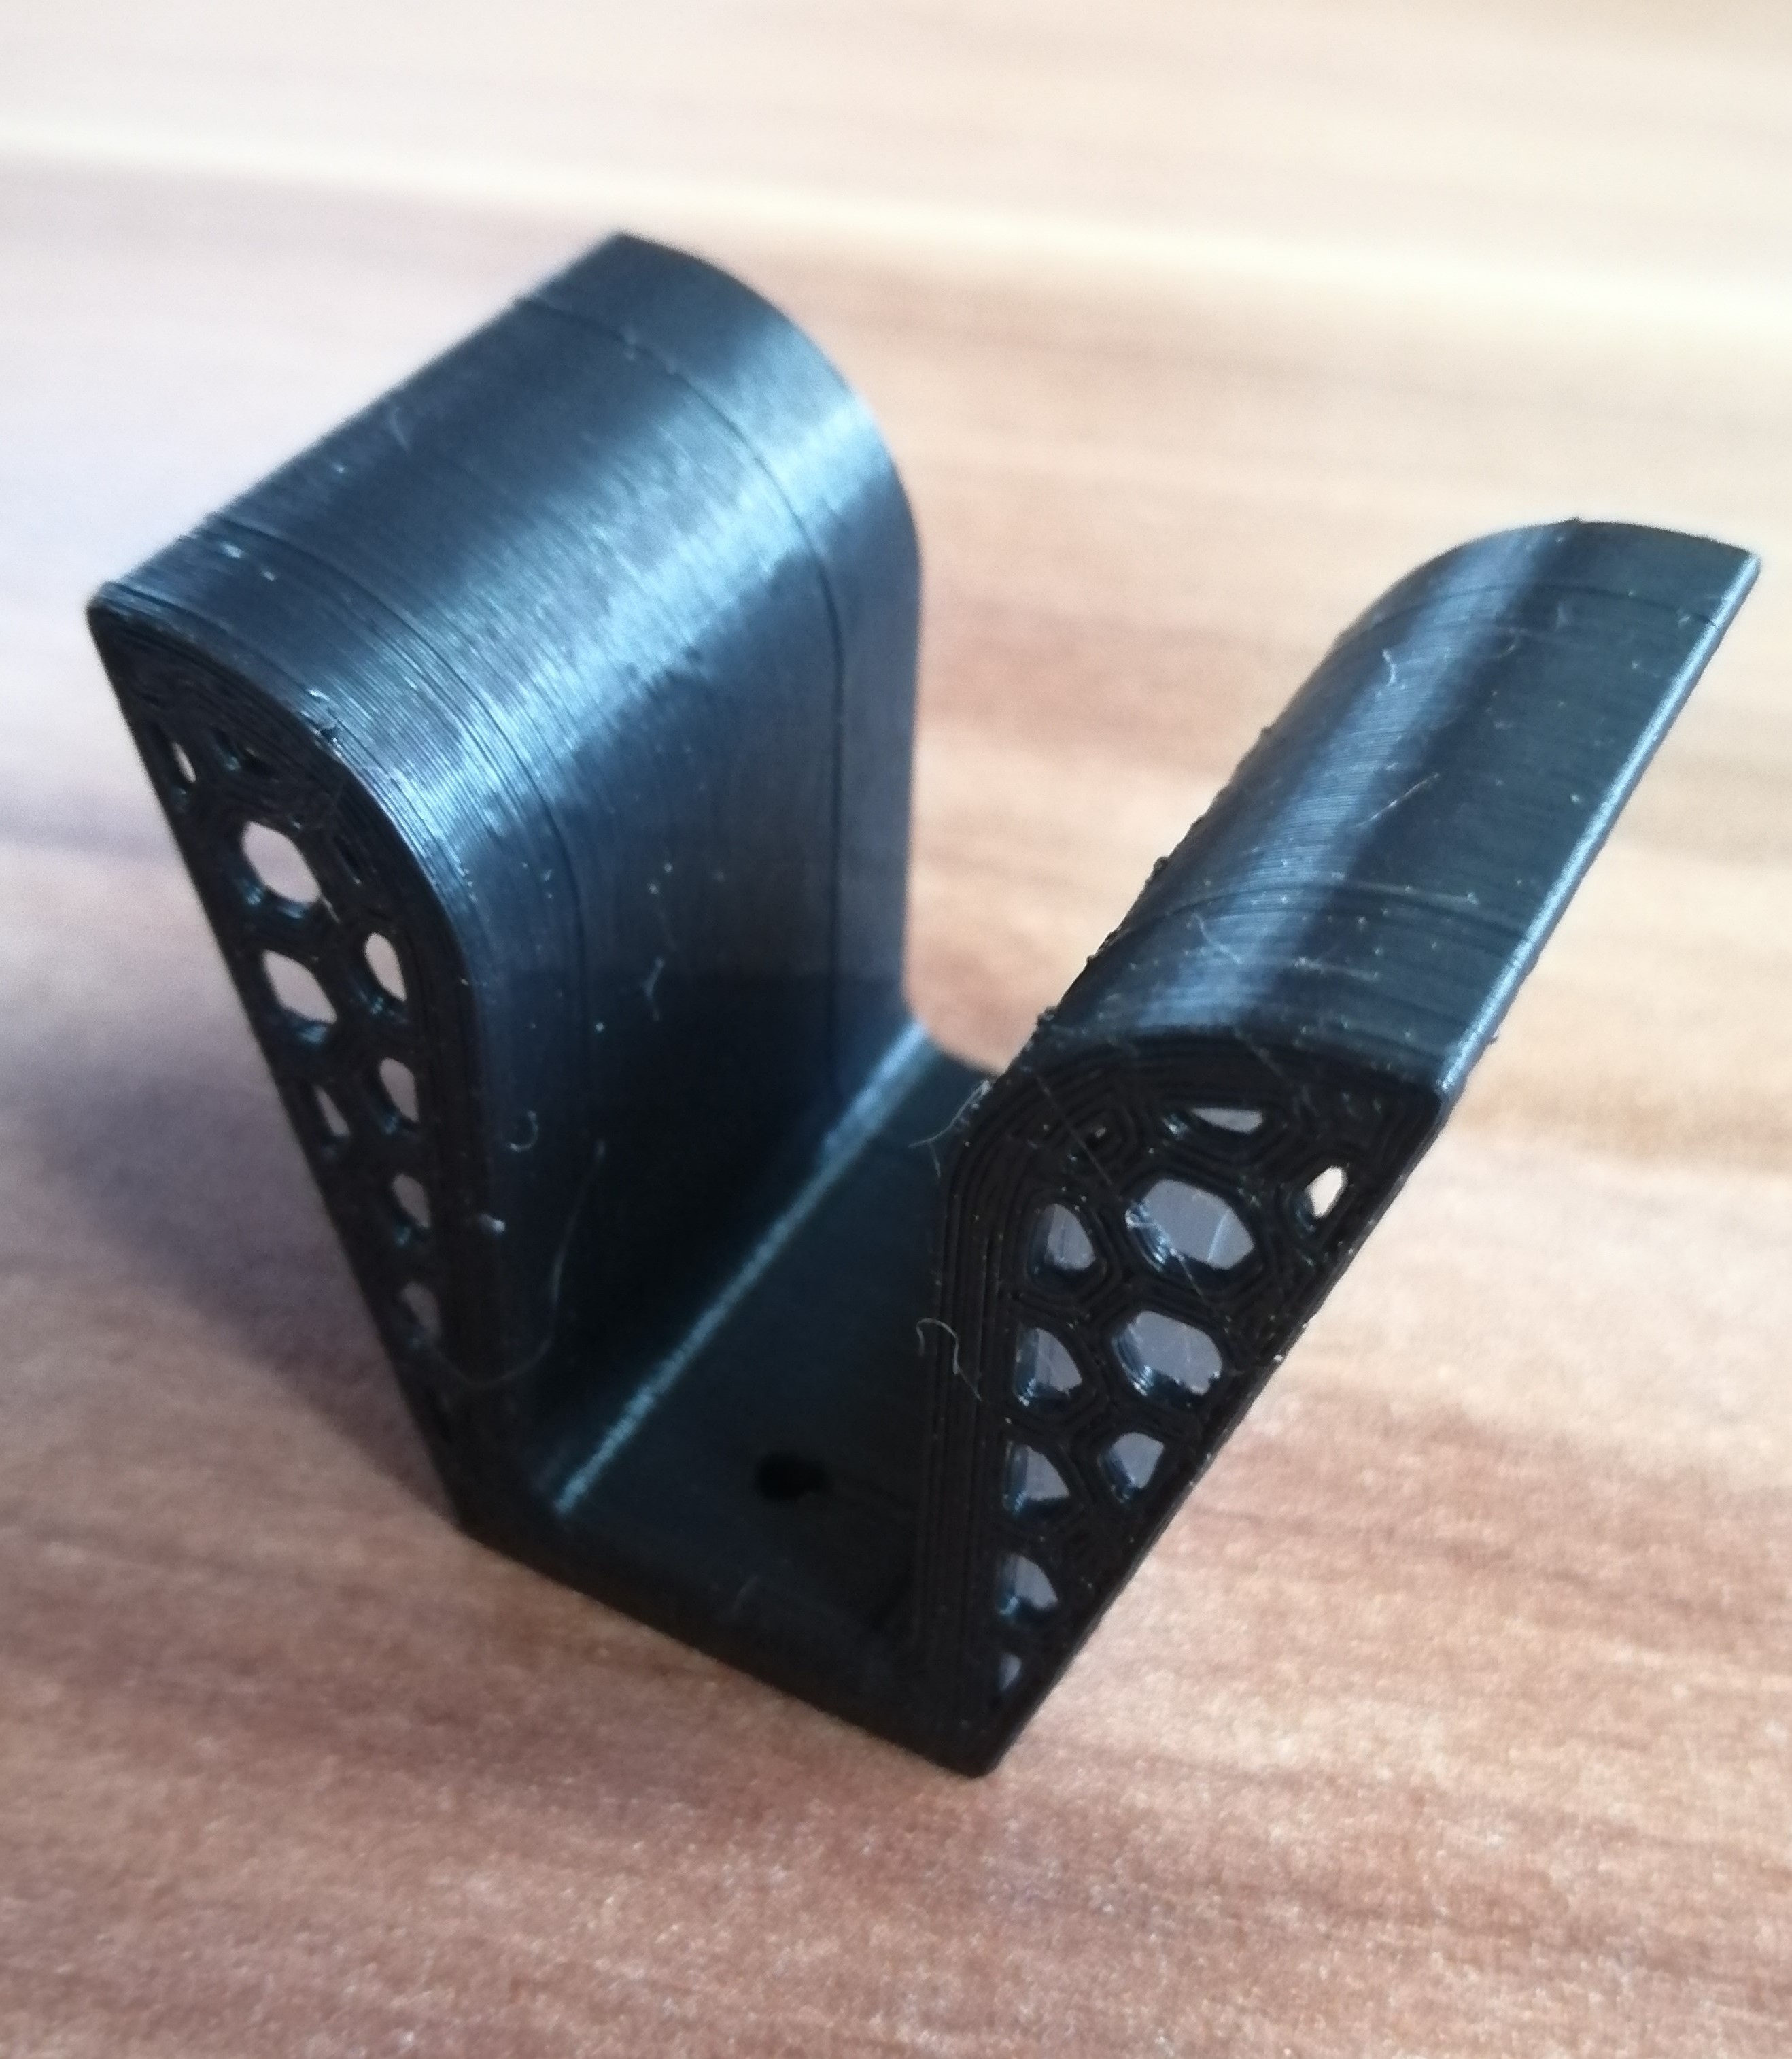
\includegraphics[width=.8\textwidth]{sec2/images/3DAnbaukomponenten/Druckbilder/AntriebsabdeckungDruck} 
\centering
\captionsetup{width=.9\textwidth}
\caption[Gedruckte Abdeckung der Antriebe]{Gedruckte Abdeckung der Antriebe}
\centering
\label{fig:DruckAntriebsabdeckung}
\end{figure}
\end{minipage}


\begin{figure}[H] %H für Positionierung hier
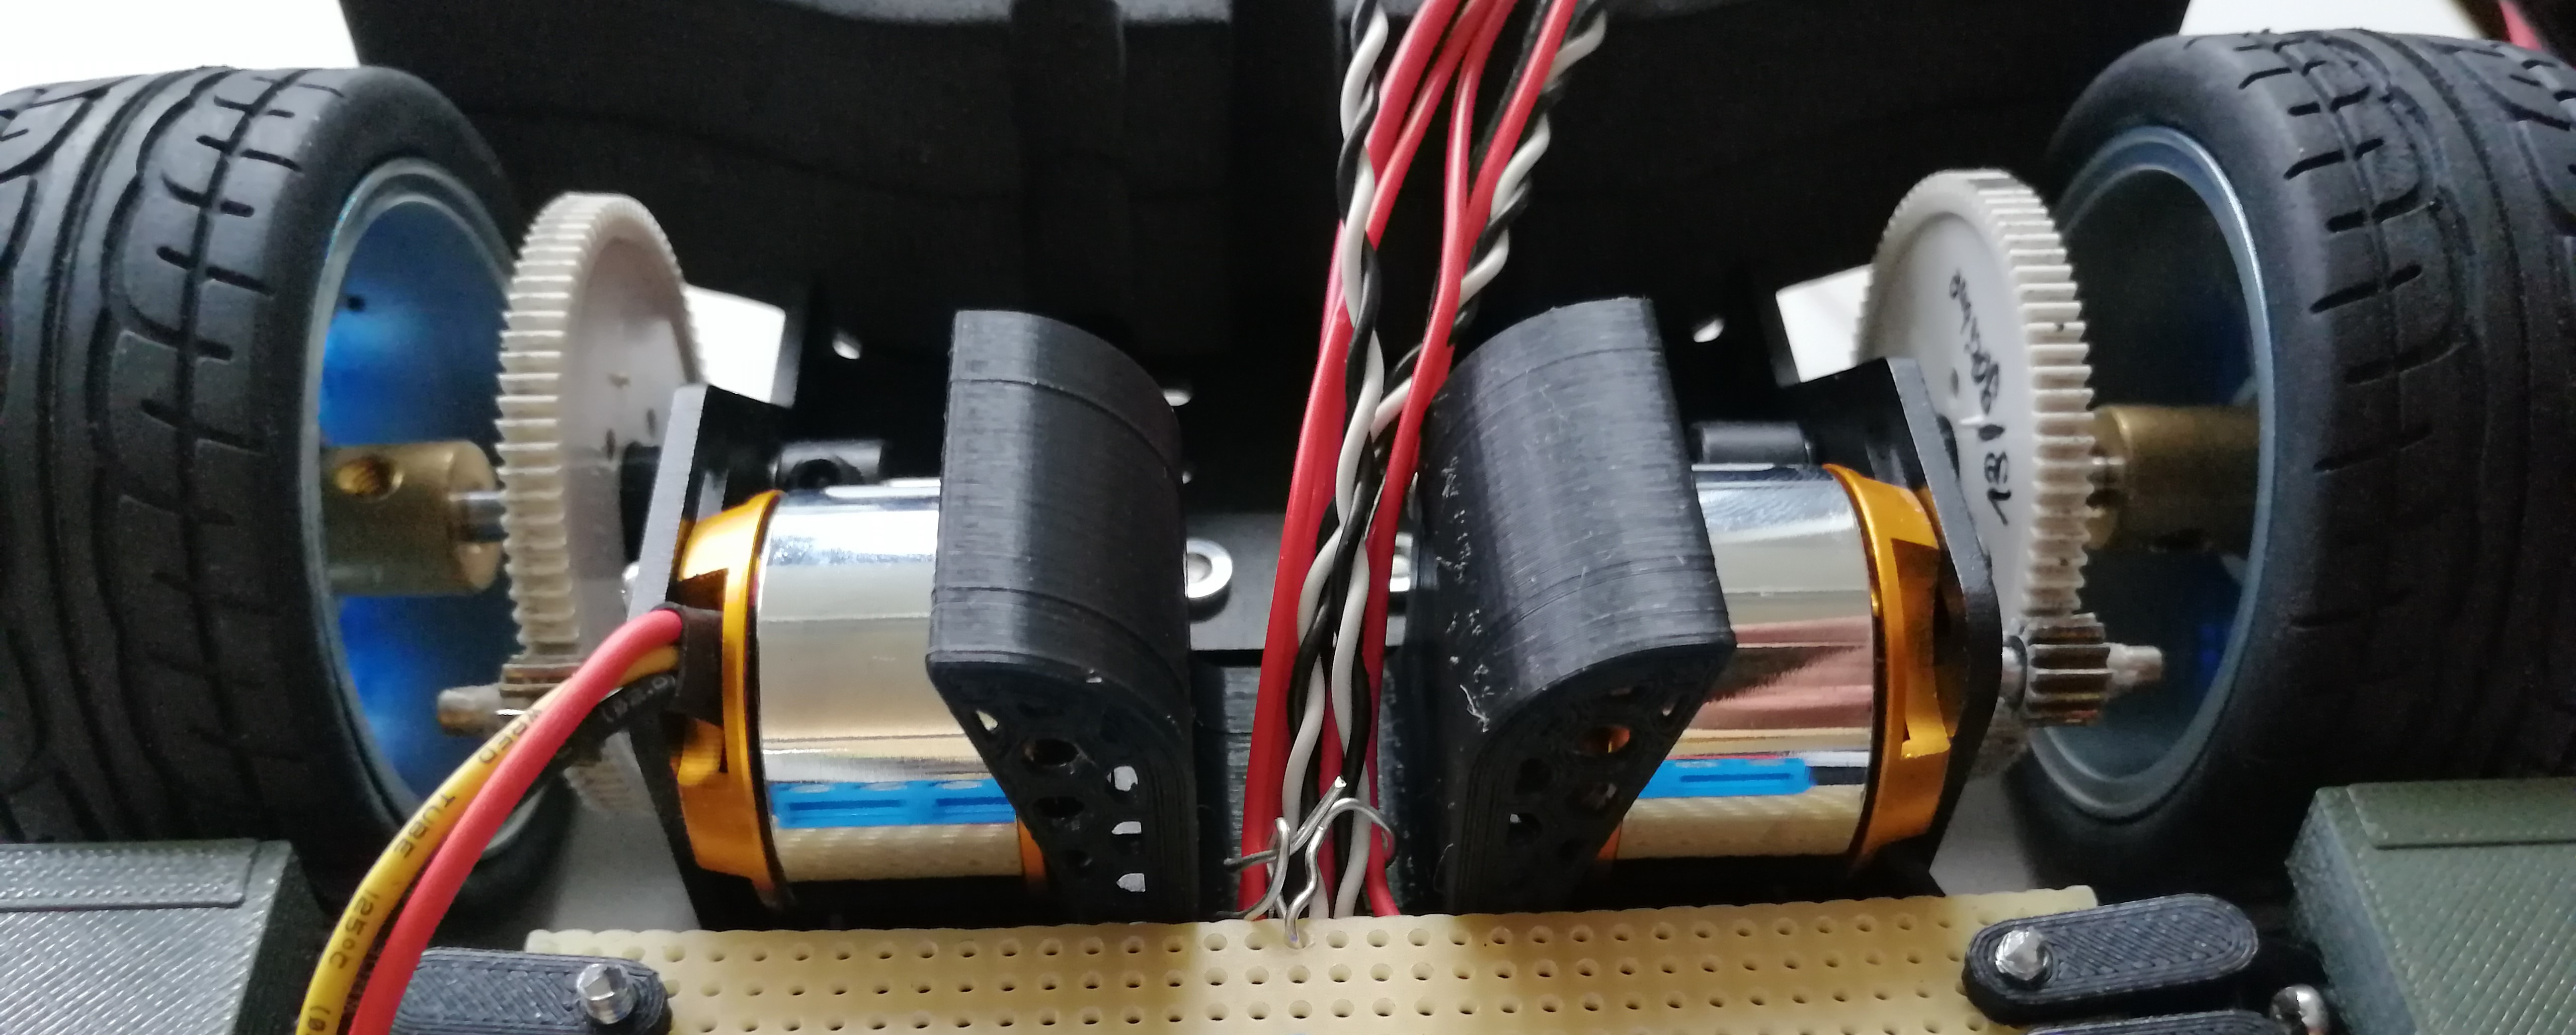
\includegraphics[width=.90\textwidth]{sec2/images/3DAnbaukomponenten/Montagebilder/AntriebsabdeckungMontage} 
\centering
\captionsetup{width=.9\textwidth}
\caption[Fertig montierte Abdeckung der Antriebe]{Fertig montierte Abdeckung der Antriebe zur Verhinderung von Reibung zwischen den Antrieben und den Kabeln, die nach oben durchgeführt werden}
\centering
\label{fig:MontageAntriebsabdeckung}
\end{figure}

\newpage

%***************************Bild Grundplatte mit Verteilerplatine/Akku/Fahrzeugperipherie fehlt
%***************************Bild obere Ebene mit Controller/Bedienung/Kamera fehlt
%***************************Änderungen müssen noch probegelesen werden
%***************************Bild der montierten ESC-Halterungen fehlt noch
%***************************Bild der montierten Verteilerplatine mit den einfachen Platinen-Halterungen fehlt noch

% Section 3 Controllerplatine und Programmiertool
%*****************************************************************
%*************************** Section 3 ***************************
%************* Controllerplatine und Programmiertool *************
%*****************************************************************


\pagestyle{fancy}
\rhead{\thepage} \chead{} \lhead{\ref{Sec3}. \nameref{Sec3}}
\cfoot{}

\section{Controllerplatine und Programmiertool}\label{Sec3}

Für dieses Projekt wird die Controllerplatine LPCXpresso54628 von NXP Semiconductors verwendet. Das Herzstück dieser Platine ist der auf dem ARM Cortex-M4 basierende Mikrocontroller LPC54628. Dieser Controller wird wegen seiner schnellen Taktfrequenz und seiner großen Anzahl an Peripherie für die Ansteuerung der Motoren und des Servos sowie für die Sensorik zur Bestimmung des Streckenverlaufs verwendet. Der Vorteil einer fertigen Controllerplatine liegt darin, dass der Schaltplan sowie das dazugehörige Layout professionell erstellt sind, wodurch dieser aufwendige Schritt bei der Entwicklung des Autos entfällt und die einwandfreie Funktionsweise des Controllers sichergestellt wird. Außerdem ist darauf bereits ein Debugger zur Programmierung und Fehlersuche verbaut. Durch das Flashen dieses Debuggers über das Programm \glqq{}LPCScrypt\_2.1.2\_57\grqq{} kann zwischen dem J-Link Debugger (Standardinstallationspfad + scripts/program\_JLINK.cmd) und dem NXP-eigenen LinkServer Debugger (Standardinstallationspfad + scripts/program\_CMSIS.cmd) gewählt werden. 

\begin{figure}[H] %H für Positionierung hier
	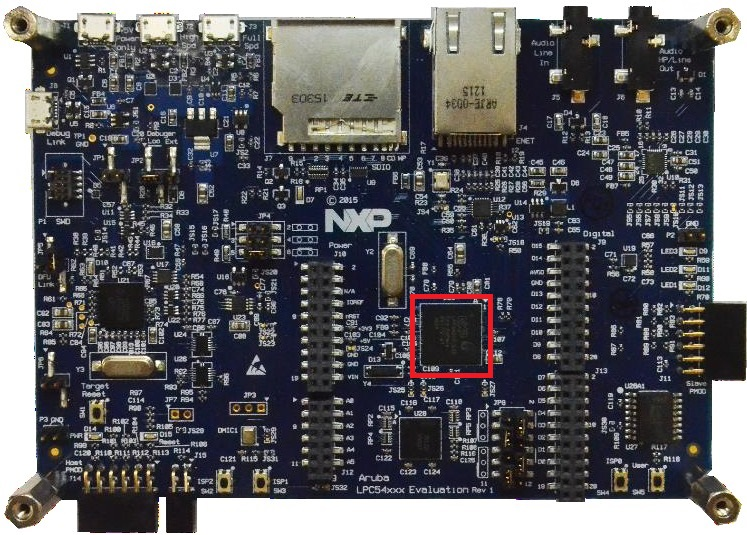
\includegraphics[width=.80\textwidth]{sec3/images/Controllerplatine} 
	\centering
	\captionsetup{width=.95\textwidth}
	\caption[Controllerplatine LPCXpresso54628 ~\protect\cite{Semic}]{Draufsicht auf die Controllerplatine mit dem Mikrocontroller LPC54628  (in rot hervorgehoben) als Hauptbestandteil ~\protect\cite{Semic}}\centering
	\label{fig:Controllerplatine}
\end{figure}

Zur Programmierung des Controllers dient das auf Eclipse basierende Tool \glqq{}MCUXpresso\grqq{}, welches von NXP Semiconductors zur Verfügung gestellt wird. Darin sind die für den verwendeten Controller notwendigen Konfigurationsdateien, wie beispielsweise das Startup-Skript und einige Beispiele, bereits enthalten. Das erleichtert den Einstieg in die Programmierung erheblich. Außerdem kann das Konfigurationstool \glqq{}MCUXpresso Config Tools\grqq{} verwendet werden. Mit diesem kann die Initialisierung der Peripheriebausteine über eine graphische Benutzeroberfläche vorgenommen werden.\vspace{11pt}

Die Pinbelegungen für die in dieser Fahrzeugversion verwendeten Peripherie (Antriebe, Servo usw.) sind im Anhang \glqq{}\nameref{SecAtt2}\grqq{} einsehbar.

\newpage
%***************************Kapitel sollte bereits passen -> nochmal absprechen

% Section 4 Antrieb des Fahrzeugs
%*****************************************************************
%*************************** Section 4 ***************************
%********************* Antrieb des Fahrzeugs *********************
%*****************************************************************


\pagestyle{fancy}
\rhead{\thepage} \chead{} \lhead{\ref{Sec4}. \nameref{Sec4}}
\cfoot{}

\section{Antrieb des Fahrzeugs}\label{Sec4}

Wie in Kapitel \ref{Sec2Sub1} beschrieben, wird das Fahrzeug von zwei \acp{BLDCMot} angetrieben, die im Folgenden genauer erklärt werden. Zusätzlich dazu wird in diesem Kapitel auch näher auf die Montage der Antriebskomponenten, die Programmierung des Antriebsbausteins, die Konfiguration der Motorcontroller und die Drehzahlmessung eingegangen.

\subsection{BLDC-Antrieb und Motorcontroller}\label{Sec4Sub1}

\acp{BLDCMot} sind im Wesentlichen wie permanent erregte Synchronmaschinen aufgebaut. Sie besitzen Magnete im Rotor und Einzelzahnwicklungen im Stator. Da solche Motoren häufig im \ac{RC}-Bereich Einsatz finden, gibt es zu deren Ansteuerung bereits vorgefertigte Bausteine, sogenannte \ac{ESC}. Diese haben zwei Signalpins für ein \ac{PWM}-Signal und zwei Anschlüsse zur Spannungsversorgung des Motorcontrollers, aus welchen die drei Strangspannungen für die Phasen des Antriebs generiert werden. Aus diesen Strangspannungen kann im übrigen auch die Motordrehzahl ermittelt werden, was im Rahmen dieser Projektarbeit auch eines der Ziele darstellt. An den Signalpins wird ein \ac{PWM}-Signal mit einer Frequenz von 50Hz angelegt, dessen Pulsbreite zwischen 1ms und 2ms liegen darf. Daraus resultiert ein Tastgrad zwischen 5\% (Stillstand) und 10\% (maximal erreichbare Drehzahl). Die maximale Drehzahl des Antriebs hängt von der Spannung des Akkus ab. Je geringer diese Spannung ist, desto geringer ist die maximal erreichbare Drehzahl. Der Anschluss der Motoren erfolgt nach der in Abbildung \ref{fig:SkizzeAntrieb} gezeigten Weise.

\begin{figure}[H] %H für Positionierung hier
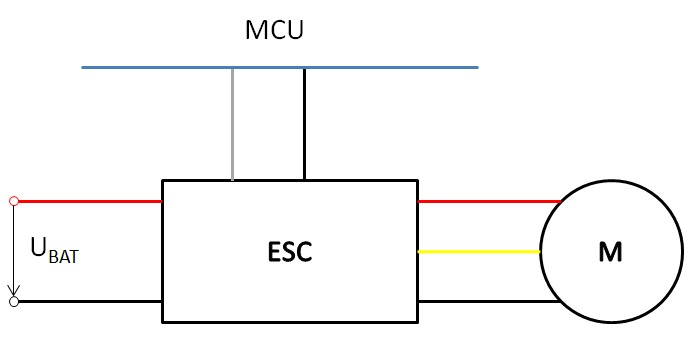
\includegraphics[width=.90\textwidth]{sec4/images/Skizze_BLDC_ESC} 
\centering
\captionsetup{width=.95\textwidth}
\caption[Skizze zur Beschaltung eines \ac{ESC}s und \ac{BLDCMot}s]{Skizze zur Beschaltung eines \ac{ESC}s und \ac{BLDCMot}s; Versorgungsspannung des \ac{ESC}s in rot und schwarz (Masse), \ac{PWM}-Signalleitungen in grau und schwarz (Masse) und Anschlussleitungen des \ac{BLDCMot}s in rot, gelb und schwarz}\centering
\label{fig:SkizzeAntrieb}
\end{figure}

\subsection{Montage der Antriebskomponenten}\label{Sec4Sub2}

Die Komponenten des Fahrzeugantriebs, welcher über zwei \acp{BLDCMot} realisiert ist, sind auf der unteren Fahrzeugebene montiert. Die Motoren selbst sind mit zwei Schrauben an der Karosserie befestigt. An der Welle der Motoren befindet sich je ein Zahnrad mit 13 Zähnen, welches ein weiteres Zahnrad mit 90 Zähnen antreibt, das an der Antriebswelle befestigt ist. Das heißt, dass sich die Reifen bei 6,923 Umdrehungen der Motorwelle genau einmal drehen.\vspace{11pt}

In Abbildung \ref{fig:MontageMotorUebersetzung} sind die montierten Komponenten des linken Antriebs abgebildet. Die Befestigungsschrauben der Motoren sind dabei in rot hervorgehoben, die Befestigungsschrauben des Zahnrads der Antriebswelle in blau und die Befestigung des Reifens in orange. Das Zahnrad der Motorwelle ist durch Erhitzen geweitet und auf die Welle aufgesetzt worden. Zur Sicherheit dient hier etwas Sekundenkleber dazu, dass sich das Zahnrad auf der Welle nicht durchdreht. Sekundenkleber ist hier völlig ausreichend, da aufgrund der Übersetzung nur 1/7 des auf die Reifen wirkenden Moments auf das Zahnrad der Motorwelle wirkt.

\begin{figure}[H] %H für Positionierung hier
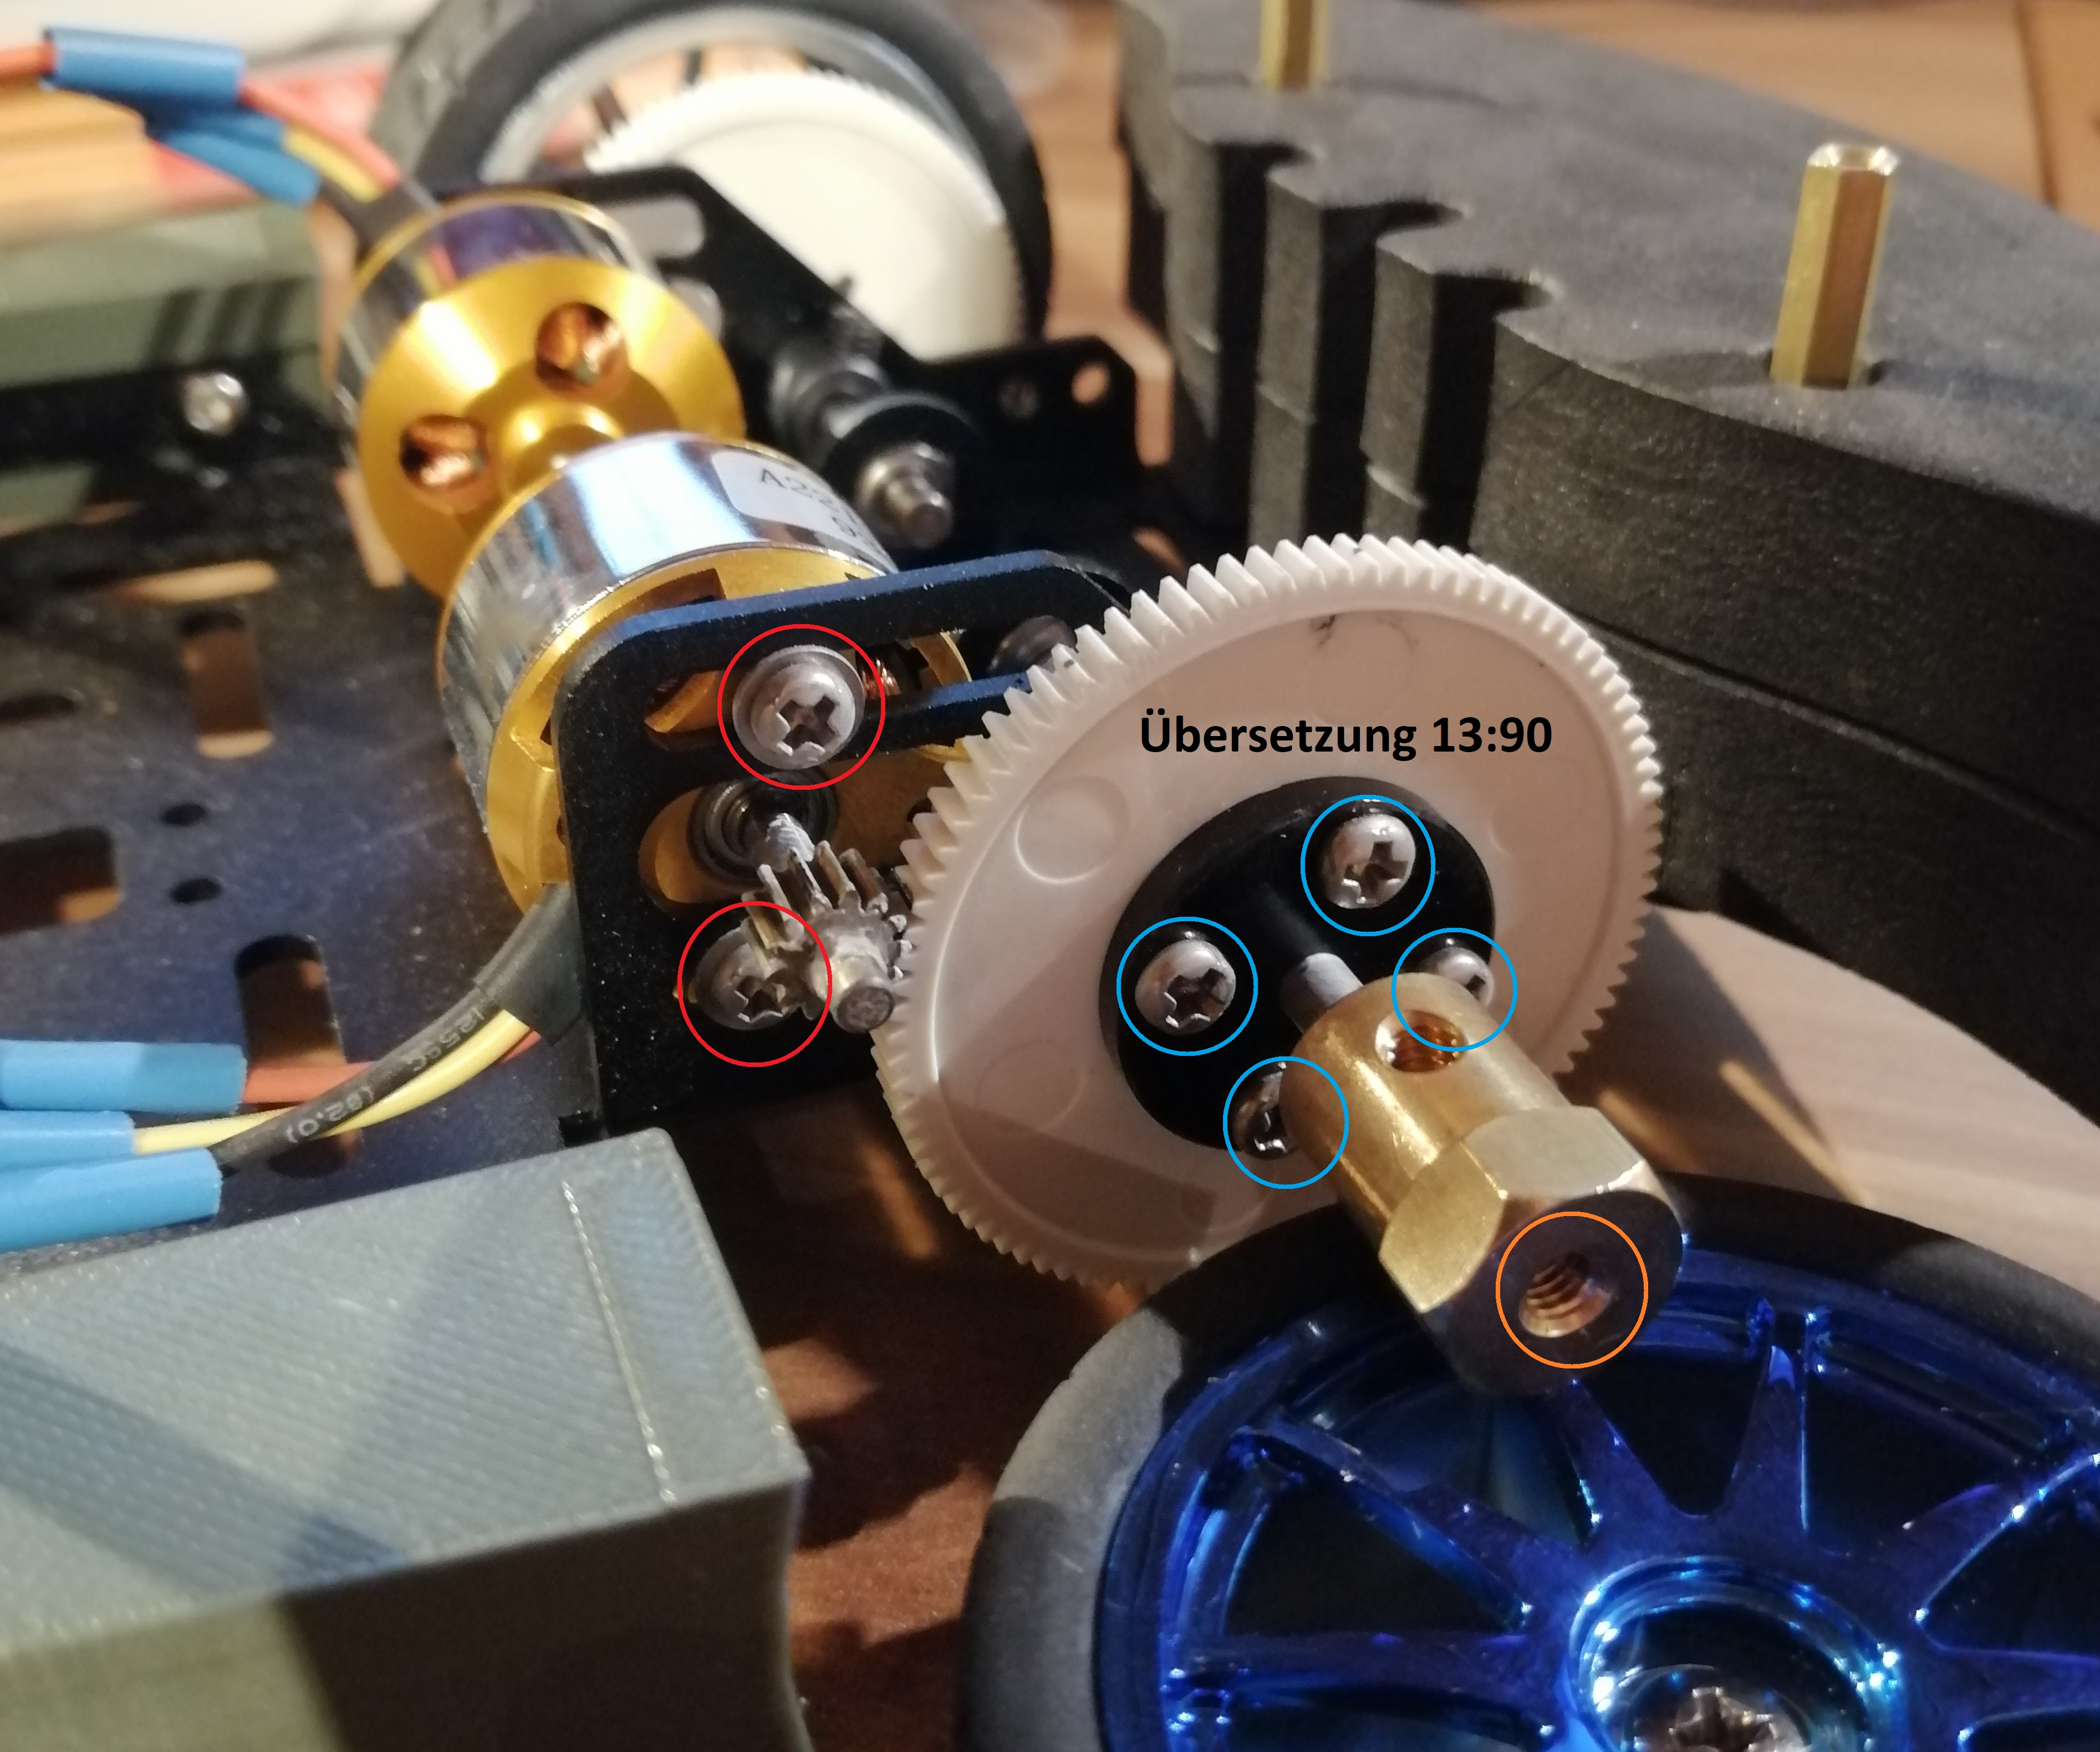
\includegraphics[width=.90\textwidth]{sec4/images/MontageMotorUebersetzung} 
\centering
\captionsetup{width=.95\textwidth}
\caption[Montage der Antriebskomponenten]{Montage der \acp{BLDCMot} und Übersetzung auf die Antriebsachse; In rot die Befestigung des \ac{BLDCMot}s, in blau die Befestigung des Zahnrads an der Antriebswelle und in orange die Befestigung des Reifens}\centering
\label{fig:MontageMotorUebersetzung}
\end{figure}

\subsection{Konfiguration der Motorcontroller}\label{Sec4Sub3}

Die beiden Motorcontroller erwarten nach dem Zuschalten der Spannungsversorgung eine Initialisierungssequenz. Das Power-On-Ereignis wird vom \ac{ESC} mit drei Tönen (tief, mittel, hoch) signalisiert. Im Anschluss daran soll der Wert an der Signalleitung größer als 0\% sein. Das bedeutet, dass ein \ac{PWM}-Signal angelegt werden muss, welches eine Drehzahl N $\geq$ 0rpm repräsentiert. Der \ac{ESC} quittiert das Erkennen des \ac{PWM}-Signals mit einem tiefen Ton. Die Initialisierungssequenz ist allerdings erst dann beendet, wenn das \ac{PWM}-Signal an der Signalleitung zuerst vergrößert und dann auf 0\% verringert wird (N = 0rpm). Dabei gibt der \ac{ESC} einen letzten, hohen Ton von sich. Der Ablauf der Initialisierungssequenz ist in Abbildung \ref{fig:initESC} dargestellt. Nach dem letzten Ton ist die Initialisierung beendet und der \ac{BLDCMot} dreht sich in Abhängigkeit des an der Signalleitung anliegenden \ac{PWM}-Signals. 

\begin{figure}[H] %H für Positionierung hier
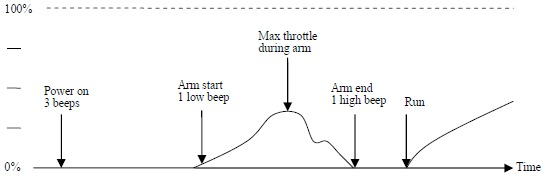
\includegraphics[width=.90\textwidth]{sec4/images/BLDCInit} 
\centering
\captionsetup{width=.95\textwidth}
\caption[Initialisierungssequenz der \ac{ESC}s]{Initialisierungssequenz der \ac{ESC}s; Wert an der Signalleitung für die Initialisierungssequenz über der Zeit; 0\% entspricht dem \ac{PWM}-Tastgrad für den Stillstand und 100\% dem für die maximal erreichbare Drehzahl}\centering
\label{fig:initESC}
\end{figure}

Da die \ac{ESC}s individuell konfiguriert werden können und in der Dokumentation zu wenige Angaben gemacht werden, ist der Tastgrad für die Werte 0\% (Stillstand) und 100\% (maximal erreichbare Drehzahl) unbekannt. Deshalb ist es nicht möglich zu wissen, welche \ac{PWM}-Tastgrade für die Initialisierungssequenz verwendet werden müssen. Über die Konfiguration der \ac{ESC}s können die Grenzen für 0\% und 100\% selbst festgelegt werden. Für das Flashen der Motorcontroller wird die Software \glqq{}BLHeliSuite\grqq{} verwendet. Die Verbindung zwischen den \ac{ESC}s und der Software stellt ein Arduino Nano her.\vspace{11pt}

Der Arduino Nano muss zuvor mit einer neuen Software beschrieben werden. Um die \ac{ESC}s flashen zu können wird der Signalpin des zu programmierenden \ac{ESC} mit dem Pin D3 und der Massepin der Signalleitung mit einem Massepin des Arduino Nano verbunden. Danach wird in der Software \glqq{}BLHeliSuite\grqq{} im Reiter \glqq{}Make Interface\grqq{} eine neue Schnittstelle erstellt (siehe Abbildung \ref{fig:ConfigBLHeliSuite}). Auf der rechten Seite des Programm-Fensters wird ein Arduino Nano als Schnittstelle eingerichtet. Mit einem Klick auf den Button \glqq{}Arduino 4way-interface\grqq{} wird die neue Software, durch die die \ac{ESC}s neu konfiguriert werden können, auf den Arduino Nano geladen.

\begin{figure}[H] %H für Positionierung hier
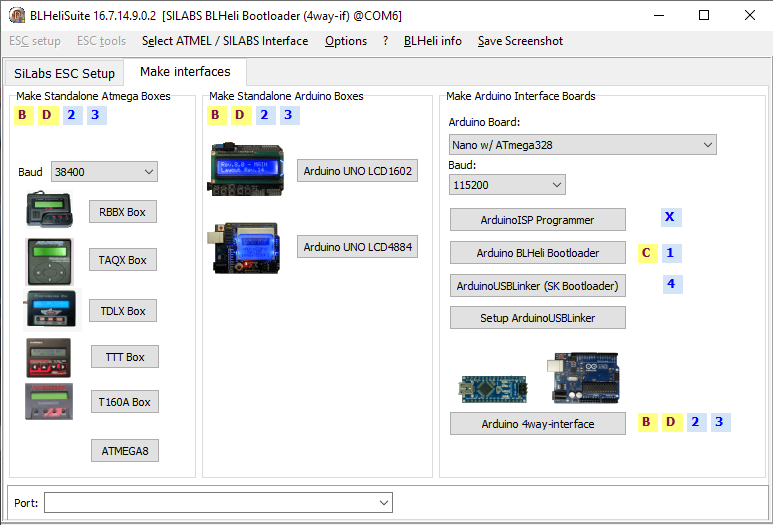
\includegraphics[width=.78\textwidth]{sec4/images/Config_BLHeliSuite} 
\centering
\captionsetup{width=.95\textwidth}
\caption[Programmierung des Arduino Nano zur \ac{ESC}-Konfiguration]{Programmierung des Arduino Nano zur \ac{ESC}-Konfiguration mit der Software BLHeliSuite}\centering
\label{fig:ConfigBLHeliSuite}
\end{figure}

Nach dem Programmieren des Arduino Nano wird die Kommunikation der BLHeliSuite-Software mit dem \ac{ESC} hergestellt. Über die Schaltfläche \glqq{}Read Setup\grqq{} werden die voreingestellten Parameter des \ac{ESC} ausgelesen. Im nächsten Schritt werden die Zeiten für die Werte \glqq{}PPM min Throttle\grqq{} (0\% Aussteuergrad) und \glqq{}PPM max Throttle\grqq{} (100\% Aussteuergrad) auf 1100µs und 1900µs angepasst. Alle vorgenommenen Einstellungen sind in Abbildung \ref{fig:BLHeliSuite} einsehbar. Die Werte werden über die Betätigung der Schaltfläche \glqq{}Write Setup\grqq{} auf den \ac{ESC} geladen. Da jetzt die Werte für 0\% und 100\% Aussteuerung bekannt sind, können die einzelnen Schritte der Initialisierung im Programm des Fahrzeugs abgearbeitet werden.

\begin{figure}[H] %H für Positionierung hier
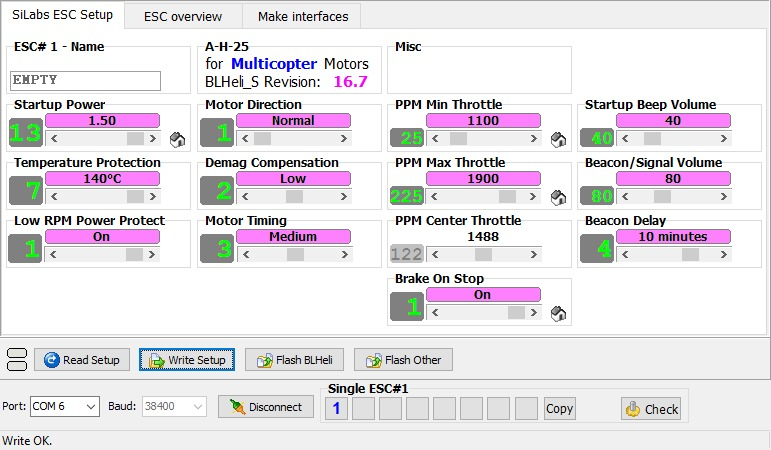
\includegraphics[width=.78\textwidth]{sec4/images/ESC_config} 
\centering
\captionsetup{width=.95\textwidth}
\caption[Parameter der neuen \ac{ESC}-Konfiguration]{Konfiguration der \ac{ESC}s mit der Software \glqq{}BLHeliSuite\grqq{}}\centering
\label{fig:BLHeliSuite}
\end{figure}

\subsection{Programmierung des Antriebsbausteins}\label{Sec4Sub4}

Der Antriebsbaustein der Software ist in zwei Dateien unterteilt, die Dateien \glqq{}drive.c\grqq{} und \glqq{}drive.h\grqq{}. Die Datei \glqq{}drive.h\grqq{} enthält alle relevanten Bibliotheken und Prototypen für die Datei \glqq{}drive.c\grqq{}.\vspace{11pt}

Außer der Einbindung der Bibliotheken und der Prototypen der Funktionen aus der Datei \glqq{}drive.c\grqq{} sind hier auch die Parameter für die Initialisierungssequenz der \ac{ESC}s und für die Initialisierung des Timers für die \ac{PWM}-Signale hinterlegt (Abbildung \ref{fig:DriveH}). 

\begin{figure}[H] %H für Positionierung hier
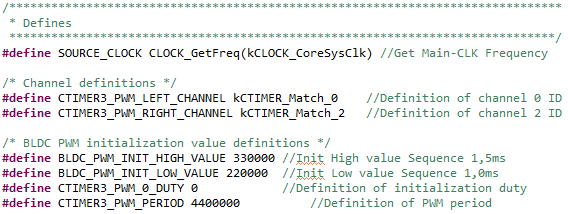
\includegraphics[width=.85\textwidth]{sec4/images/DriveH} 
\centering
\captionsetup{width=.95\textwidth}
\caption[Relevante Zeilen der Datei \glqq{}drive.h\grqq{}]{Relevante Zeilen der Datei \glqq{}drive.h\grqq{} mit den Parametern für die Initialisierungssequenz der \ac{ESC}s und für die Initialisierung des \ac{PWM}-Timers}\centering
\label{fig:DriveH}
\end{figure}

Für die \ac{PWM}-Periodendauer wird bei der Initialisierung ein Wert von 4.400.000 Takten festgesetzt, woraus mit einer \ac{CPU}-Taktfrequenz von 220MHz (220.000.000 Takte pro Sekunde) eine Periodendauer von 20ms resultiert. Die Pulsbreite wird während des Programmablaufs regelmäßig überschrieben.\vspace{11pt}

Der \ac{ESC}-Initialisierungswert für den Stillstand (\glqq{}BLDC\_PWM\_INIT\_LOW\_VALUE\grqq{}, 220.000) entspricht hier einer \ac{PWM}-Pulsbreite von 1,0ms und der Initialisierungswert für die in etwa mittlere Aussteuerung (\glqq{}BLDC\_PWM\_INIT\_HIGH\_VALUE\grqq{}, 330.000) einer Breite von 1,5ms. Die volle Aussteuerung der Motoren wird, wie über die \glqq{}BLHeliSuite\grqq{} festgelegt, bei einer Pulsdauer von 1,9ms erreicht (BLDCMaxValue, ca. 418.000). Eine Drehzahl von N = 0rpm wird theoretisch über die bei der \ac{ESC}-Konfiguration festgelegten 1,1ms ermöglicht (242.000). Da das \ac{PWM}-Signal leicht abweicht, wird ein etwas geringerer Wert veranlagt (BLDCMaxValue, ca. 240.000 = 1,09ms). Damit wird sichergestellt, dass sich die Räder im Stillstand nicht drehen.\vspace{11pt}

Die Parameter BLDCMaxValue und BLDCMinValue existieren im Code für die linke und rechte Antriebsseite separat (\glqq{}BLDCLeftMaxValue\grqq{}, \glqq{}BLDCLeftMinValue\grqq{} \& \glqq{}BLDCRightMaxValue\grqq{}, \glqq{}BLDCRightMinValue\grqq{}). Die Werte dieser Parameter kommen direkt aus dem \ac{EEPROM} und können mit dem Bedienungsboard eingestellt werden (siehe Abbildung \ref{fig:DriveC0}).\vspace{11pt}

\begin{figure}[H] %H für Positionierung hier
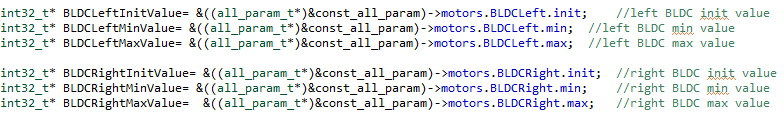
\includegraphics[width=.95\textwidth]{sec4/images/DriveC0} 
\centering
\captionsetup{width=.95\textwidth}
\caption[Extremwerte der Antriebsgeschwindigkeit als Parameter aus dem \ac{EEPROM}]{Extremwerte der Antriebsgeschwindigkeit als Parameter aus dem \ac{EEPROM}, deren Werte über das Bedienungsboard individuell einstellbar sind; Teil der Datei \glqq{}drive.c\grqq{}}\centering
\label{fig:DriveC0}
\end{figure}

Auch die beiden \ac{PWM}-Timer (einer je Motorcontroller) benötigen bei der Initialisierung einige Parameter, deren Werte in der Datei \glqq{}drive.h\grqq{} festgelegt sind (PWM-Periodendauer, \ac{PWM}-Pulsdauer, Channel). Die Channel werden auf das Timer Match Register 2 (rechter Antrieb, \glqq{}kCTIMER\_Match\_2\grqq{}) und auf das Timer Match Register 0 (linker Antrieb, \glqq{}kCTIMER\_Match\_0\grqq{}) festgelegt, was bei dem verwendeten Controller den Pins P0.27 (rechts) und P3.10 (links) entspricht. Der Pin P3.10 wird auf der Controllerplatine über den Pin 7 und der Pin P0.27 über den Pin 12 der Buchsenleiste J13 nach außen geführt. Der Anschluss der Motorcontroller ist über den Anhang \glqq{}\nameref{SecAtt1}\grqq{} nachvollziehbar.\vspace{11pt}

\begin{figure}[H] %H für Positionierung hier
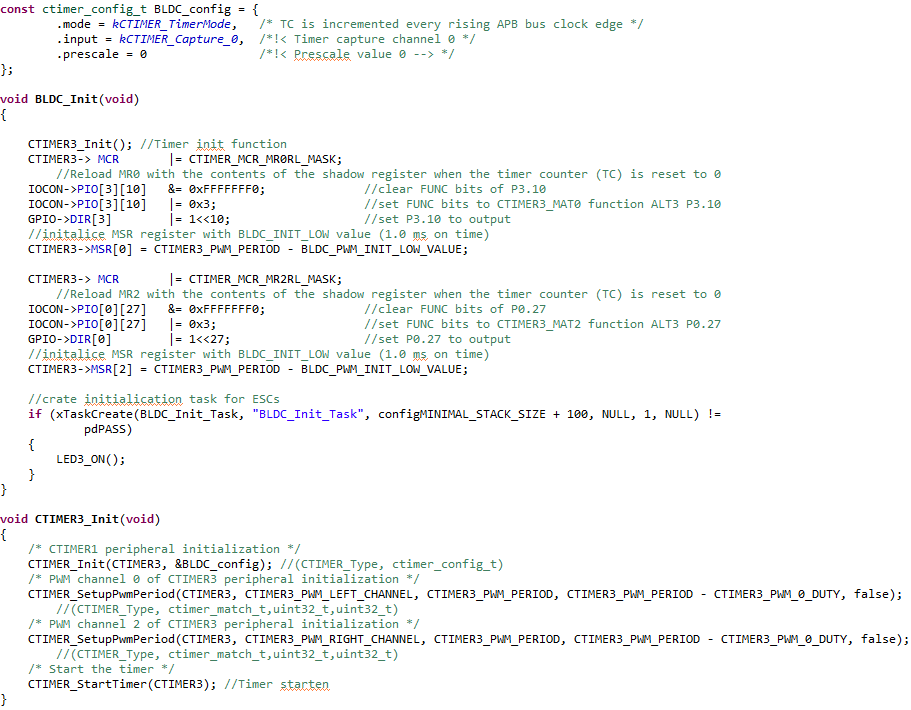
\includegraphics[width=.95\textwidth]{sec4/images/DriveC1} 
\centering
\captionsetup{width=.95\textwidth}
\caption[Funktionen BLDC\_Init und CTIMER3\_Init der Datei \glqq{}drive.c\grqq{}]{Funktionen BLDC\_Init und CTIMER3\_Init der Datei \glqq{}drive.c\grqq{}}\centering
\label{fig:DriveC1}
\end{figure}

Die Datei \glqq{}drive.c\grqq{} enthält die Funktionen zur Initialisierung der für die Verwendung der Antriebe notwendigen Controller-Peripherie (siehe Abbildung \ref{fig:DriveC1}) und zur Initialisierung der Motorcontroller (siehe Abbildung \ref{fig:DriveC2}).\vspace{11pt}

In der Funktion BLDC\_Init wird zuerst die Funktion CTIMER3\_Init aufgerufen, welche die beiden vorher festgelegten Kanäle des Timers C3 (\glqq{}kCTIMER\_Match\_0\grqq{} und \glqq{}kCTIMER\_Match\_2\grqq{}) mit den in der Datei ''drive.h'' festgelegten Parametern als \ac{PWM}-Timer mit einer Periodendauer von 20ms und einer Pulsdauer von 0ms initialisiert. Im Anschluss daran wird einzeln für beide Kanäle festgelegt, dass bei einem Timer-Überlauf die neuen Daten für die Pulslängen aus den Shadow-Registern geladen werden sollen. Zum Ändern der Geschwindigkeit eines der beiden Antriebe muss deshalb lediglich ein neuer Wert in das Shadow-Register geschrieben werden. Hier muss allerdings aufgepasst werden, da das Register nicht die Pulsbreite (On-Time) sondern die Off-Time erwartet. Deshalb muss der Wert, der eingetragen wird, der Periodendauer abzüglich der Pulsdauer entsprechen. Zusätzlich werden in der Funktion BLDC\_Init auch die Pins P3.10 und P0.27 für die Verwendung als \ac{PWM}-Ausgang des Timers C konfiguriert. Am Ende wird noch der erste \ac{ESC}-Initialisierungswert in die beiden Shadow-Register geschrieben, bevor die \ac{ESC}-Initialisierungsfunktion aufgerufen wird (siehe Abbildung \ref{fig:DriveC2}).

\begin{figure}[H] %H für Positionierung hier
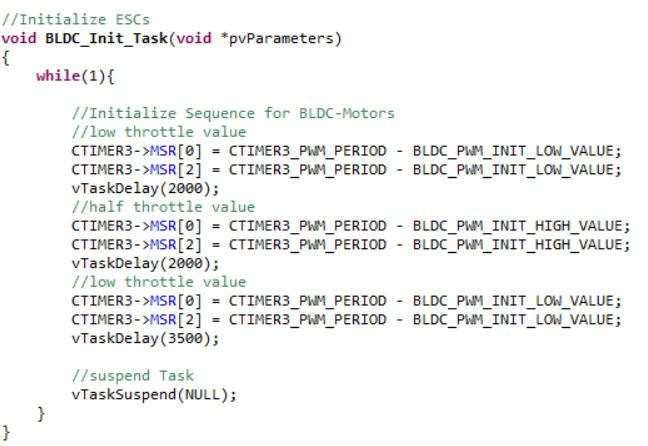
\includegraphics[width=.9\textwidth]{sec4/images/DriveC2} 
\centering
\captionsetup{width=.95\textwidth}
\caption[Funktion BLDC\_Init\_Task der Datei \glqq{}drive.c\grqq{}]{Funktion BLDC\_Init\_Task der Datei \glqq{}drive.c\grqq{} zum Durchlaufen der Initialisierungssequenz der \ac{ESC}s}\centering
\label{fig:DriveC2}
\end{figure}

Der Task BLDC\_Init\_Task beginnt mit dem Befüllen der Shadow-Register mit dem ersten Initialisierungswert. Nach einer Wartezeit von 2s wird der zweite Initialisierungswert in die Register geschrieben. Ebenfalls nach einer Zeit von 2s wird dann wieder der erste Initialisierungswert in die Shadow-Register geschrieben und die Initialisierung der \ac{ESC}s ist abgeschlossen. Die Wartezeiten sind notwendig, damit die \ac{ESC}s Zeit haben, die Änderungen zu erfassen.



\newpage
\subsection{Drehzahlmessung}\label{Sec4Sub5}

Im folgenden Abschnitt zur Drehzahlmessung werden deren Notwendigkeit sowie Entwicklungsschritte und Realisierung erarbeitet. Des weiteren wird auch ein Ausblick für die Weiterentwicklung Schaltung gegeben.

\subsubsection{Erörterung der Notwendigkeit einer Drehzahlmessung}\label{Sec:NotwendigkeitDrehzahlmessung}

Die Quellspannung von Akkus verringert sich mit steigender Betriebszeit, weshalb bereits bei vorherigen Fahrzeug-Versionen eine Drehzahlmessung benötigt wurde, um über eine Regelung die Spannungsabhängigkeit der Drehzahl bei \acp{DCMot} ausgleichen zu können. Die Spannungsabhängigkeit von \acp{DCMot} bereitet insbesondere beim Überfahren eines Hügels Probleme. Da die in den vorangegangenen Fahrzeugmodellen verwendeten \acp{DCMot} durch \acp{BLDCMot} ersetzt wurden, stellt sich allerdings erneut die Frage nach der Notwendigkeit einer Drehzahlmessung. Die Variation der Drehzahl erfolgt bei \acp{DCMot} über die Änderung der Betriebsspannung, was auch die Abhängigkeit von der Versorgungsspannung erklärt. Die Drehzahlvariation bei einem \ac{BLDCMot} wird hingegen über eine Frequenzänderung der Strangspannungen realisiert. Zur Klärung der Frage nach einer Spannungsabhängigkeit der \acp{BLDCMot}, ist eine Messung am Prüfstand erforderlich.\vspace{11pt}

Für die Durchführung der Messung wird ein bereits vorhandener Prüfstand für Modellfahrzeuge verwendet (siehe Abbildung \ref{fig:Pruefstand01}), welcher im Rahmen einer Bachelor-Abschlussarbeit an der HAW Landshut erstellt wurde. Damit das Fahrzeug möglichst stabil auf dem Prüfstand steht und die Räder des Fahrzeugs ihre Rotationsbewegung besser auf die \acp{DCMot} des Prüfstands übertragen können, wird das Heck des Fahrzeugs mit Hilfe eines Drahtes am Prüfstand befestigt (Abbildung \ref{fig:Pruefstand01} blaue Markierung). Die vorderen Räder des Fahrzeuges sind ebenfalls am Prüfstand fixiert (Abbildung 44 gelbe Markierungen). 

\begin{figure}[H] %H für Positionierung hier
\includegraphics[width=.73\textwidth]{sec4/images/Pruefstand_Messung_UAbhängigkeit} 
\centering
\captionsetup{width=.95\textwidth}
\caption[Messaufbau zur Prüfung der Spannungsabhängigkeit der \acp{BLDCMot}]{Messaufbau zur Prüfung der Spannungsabhängigkeit der \acp{BLDCMot}; in blau die Befestigung des Hecks an der Grundplatte des Prüfstands, in gelb die Befestigung der Vorderreifen am Prüfstand, in rot die DC-Motoren zur Spannungsmessung}\centering
\label{fig:Pruefstand01}
\end{figure}

Zur Überprüfung einer eventuellen Abhängigkeit der Drehzahl von der Versorgungsspannung, wird die Spannung an den vorhandenen \acp{DCMot} des Prüfstands gemessen, da diese direkt proportional zur Drehzahl ist (siehe Gleichung \ref{eq4.1}). Die Abhängigkeit der gemessenen Spannung von der Drehzahl ist allerdings nur annähernd linear, da die Drehmomentkonstante k\textsubscript{i} bei hohen Drehzahlen leicht einbricht. Aufgrund der für die Messung konstant eingestellten Pulsbreite von 1,5ms, spielt der Einbruch der Drehmomentkonstante allerdings keine große Rolle, da sich die Drehzahl, wenn überhaupt, nur sehr gering ändert. Dieser Zusammenhang kann deshalb vereinfachend als linear angenommen werden.\vspace{11pt}

Die Versorgungsspannung der \acp{ESC} wird für die Aufnahme verschiedener Messwerte zwischen 6,1V und 8V variiert. Ändert sich die gemessene Spannung mit der Variation der Versorgungsspannung, so ist das ein hinreichender Beweis dafür, dass die Drehzahl der \acp{BLDCMot} spannungsabhängig ist. Die Ergebnisse der Messreihe aus Tabelle \ref{tab:PruefstandMess01} sind zur einfacheren Auswertung in Abbildung \ref{fig:Pruefstand02} visualisiert.

\begin{equation}\label{eq4.1}
U_A = k_i \cdot N \cdot \frac{\pi}{30}
\end{equation}

\begin{table}[H]
\begin{tabular}{|c|c|c|c|c|c|c|c|c|c|c|}
\hline
\rule{0pt}{15pt} Messung & 1&2&3&4&5&6&7&8&9&10 \\
\hline
U\textsubscript{Versorgung} [$V$]&8.0&7.9&7.8&7.7&7.6&7.5&7.4&7.3&7.2&7.1 \\ 
\hline
U\textsubscript{Messung} [$V$]&5.80&5.75&5.65&5.57&5.48&5.40&5.35&5.25&5.18&5.09 \\
\hline
\hline
\rule{0pt}{15pt} Messung & 11&12&13&14&15&16&17&18&19&20 \\
\hline
U\textsubscript{Versorgung} [$V$]&7.0&6.9&6.8&6.7&6.6&6.5&6.4&6.3&6.2&6.1 \\ 
\hline
U\textsubscript{Messung} [$V$]&5.05&4.96&4.87&4.82&4.69&4.73&4.66&4.60&4.50&4.45 \\
\hline
\end{tabular}
\centering
\captionsetup{width=.95\textwidth}
\caption[Messreihe 1: Spannungsabhängigkeit Drehzahl]{Messreihe 1: Messwerte für Überprüfung einer eventuellen Spannungsabhängigkeit der Drehzahl}\centering
\label{tab:PruefstandMess01}
\end{table}

Aus Abbildung \ref{fig:Pruefstand02} kann die Erkenntnis abgeleitet werden, dass die Drehzahl der \acp{BLDCMot}, welche proportional zu der an den \acp{DCMot} gemessenen Ankerspannung U\textsubscript{Messung} ist, bei einem Abfallen der Versorgungsspannung nicht konstant bleibt, denn andernfalls wäre die resultierende Gerade eine Horizontale. Deshalb ist die Drehzahl der \acp{BLDCMot} wie die der \acp{DCMot} abhängig von der Versorgungsspannung.\vspace{11pt}

Die sich aus der Messreihe ergebende Erkenntniss, führt zu dem Entschluss, dass eine Drehzahlregelung nicht nur sinnvoll, sondern auch erforderlich ist. Denn während der Durchfahrt des Parcours wird nicht zu jedem Zeitpunkt die volle Drehzahl benötigt. Folglich hat eine Regelung den Vorteil, dass die vorgegebene Drehzahl auch bei einer fortschreitenden Entladung des Akkus weiterhin aufrecht gehalten werden kann. Wird eine feste Geschwindigkeit vorgegeben, kann die Regelung bei fallender Versorgungsspannung der \acp{ESC} das \ac{PWM}-Signal bis zur Stellgrenze (Pulsbreite = 1,9ms) erhöhen. Erst bei Erreichen der Stellgrenze nimmt die Drehzahl linear mit der Versorgungsspannung ab.

\begin{figure}[H] %H für Positionierung hier
\includegraphics[width=.90\textwidth]{sec4/images/PruefstandMess02} 
\centering
\captionsetup{width=.95\textwidth}
\caption [Spannungsabhängigkeit der Drehzahl von der Versorgungsspannung]{Spannungsabhängigkeit der Drehzahl der \acp{BLDCMot} von der Versorgungsspannung}\centering
\label{fig:Pruefstand02}
\end{figure}

Des weiteren muss das Fahrzeug im Rahmen des NXP-Cups nach dem Überfahren der Ziellinie innerhalb von zwei Metern anhalten können. In der Konfiguration der \acp{ESC} bietet sich dafür die Einstellung \glqq{}Break On Stop\grqq{} an, mit der das Fahrzeug bei einer PWM-Pulsdauer von 1,1ms (BLDCMinValues: BLDCLeftMinValue, BLDCRightMinValue) aktiv bremst, indem die drei Phasen der \acp{BLDCMot} auf Masse geschlossen werden.\vspace{11pt}

Zur Verifizierung eines ordnungsgemäßen Bremsverhaltens, wird eine Probefahrt auf einer langen geraden Strecke an der HS-Landshut durchgeführt. Die Antriebe sind dabei so konfiguriert das sich das Fahrzeug nach der Initialisierung der \acp{BLDCMot} unmittelbar mit maximaler Geschwindigkeit fortbewegt und nach kurzer Fahrtdauer (ca. 3s) stoppt (BLDCMinValues). Hierbei stellt man fest, dass die Bremskraft ausreicht, um das Fahrzeug innerhalb von ca. 30 cm zum Stehen zu bringen.\vspace{11pt}

Während des Testens fällt auf, dass sich die Reifen trotz gleicher ESC-Konfiguration unterschiedlich schnell drehen. Der Grund für dieses Problem lässt darauf schließen, dass die beiden Antriebsseiten einen unterschiedlichen Reibungswert aufweisen. Das kann daran liegen, dass bei den Achsen keine Lager verwendet werden und bei der Übersetzung das Getriebespiel (zwischen den Zahnrädern) auf beiden Antriebsseiten unterschiedlich groß ist, was ebenfalls die Reibung beeinflusst.\vspace{11pt}
%Zum anderen wird davon ausgegangen, dass bei minimalen und maximalen Antrieb die Stellgrenzen (1,09ms und 1,9ms) sprich die ON-Zeit des PWM-Signals kurzfristig über- bzw. unterschritten wird. Befindet sich die Pulsbreite außerhalb des konfigurierten Bereiches schaltet der Antrieb kurzweilig aufgrund des undefinierten Signalzustandes ab und bei Rückkher in den definierten Bereich wieder an.\vspace{11pt} 

Die Spannungsabhängigkeit der \acp{BLDCMot} sowie das unterschiedliche und reibungsabhängige Drehverhalten der beiden Antriebe, machen eine Drehzahlregelung zwingend erforderlich, um ein zuverlässiges und sicheres Fahrverhalten zu gewährleisten.

\subsubsection{Auswahl des Messprinzips}\label{Sec4Sub5Sub2}

Nachdem bereits festgestellt werden konnte, dass eine Drehzahlregelung der \acp{BLDCMot} erforderlich ist, gilt es in diesem Abschnitt entsprechende Messprinzipien zur Drehzahlerfassung gegenüberzustellen und die für dieses Projekt sinnvollste Messmethode zu bestimmen.\vspace{11pt}

Die in bisherigen Fahrzeugversionen am häufigsten verwendeten Methoden zur Drehzahlerfassung sind die Verwendung von Hallsensoren oder Lichtschranken (siehe Abbildung \ref{fig:Vorgaengerfahrzeug}). Hallsensoren und Lichtschranken eignen sich hervorragend für eine berührungslose Drehzahlerfassung. Für die Drehzahlmessung mithilfe von Hallsensoren werden kleine Magnete auf der Innenseite der Hinterräder angebracht, welche vom Hallsensor erfasst werden (Abbildung \ref{fig:Vorgaengerfahrzeug}, links). Anhand der Zeit zwischen den Zuständen \glqq{}Magnet vorhanden\grqq{} oder \glqq{}Magnet nicht vorhanden\grqq{} (High/Low-Signal), kann unter Berücksichtigung der jeweiligen Getriebeübersetzung und Menge der Magnete die Drehzahl der \acp{BLDCMot} bestimmt werden. Die Drehzahlmessung mit einer Lichtschranke funktioniert in der Auswertung genau wie die Messung mit  Hallsensoren, lediglich die Messmittel sind anders (Abbildung \ref{fig:Vorgaengerfahrzeug}, rechts).

\begin{figure}[H] %H für Positionierung hier
\includegraphics[width=.45\textwidth]{sec4/images/Vorgängerfahrzeug} 
\includegraphics[width=.45\textwidth]{sec4/images/Vorgängerfahrzeug_zwei} 
\captionsetup{width=.95\textwidth}
\centering
\caption[Varianten der Drehzahlerfassung bei vorherigen Fahrzeugversionen]{Varianten der Drehzahlerfassung bei vorherigen Fahrzeugversionen; links: Hallsensoren; rechts: Lichtschranke}\centering
\label{fig:Vorgaengerfahrzeug}
\end{figure}     


Ein Hallsensor bietet den Vorteil, dass neben der Erfassung der Drehzahl auch die Drehrichtung mit Hilfe eines zweiten um 90° versetzten Hallsensors bestimmt werden kann. Dazu muss nicht einmal ein zweiter Sensor gekauft werden, da bereits zwei Sensoren mit 90°-Versetzung in einem Hallsensorgehäuse verbaut sind. Im Zuge dieser Projektarbeit ist eine Erfassung der Drehrichtung jedoch nicht erforderlich, da die für die \acp{BLDCMot} verwendeten \acp{ESC} so konfiguriert sind, dass nur eine Fahrt in Vorwärtsrichtung möglich ist. Ein weiterer Vorteil des Hallsensors aber auch einer Lichtschranke ist, dass die für die GPIO-Pins notwendigen Rechtecksignale direkt vorgegeben werden und keine zusätzliche Umformung des Signals mehr notwendig ist. \vspace{11pt}

Aufgrund der Klebebefestigung der Magnete besteht das Risiko, dass diese sich nach einer gewissen Zeit ablösen und somit die Daten zur Drehzahlerfassung verfälschen. Wie in Abbildung \ref{fig:Vorgaengerfahrzeug} zusätzlich zu erkennen ist, ist die Montage des Hallsensors, die lediglich über die Versorgungsdrähte oder eine zusätzliche Drahtstütze realisiert ist, sehr anfällig auf Erschütterungen. Eine zuverlässige und weniger erschütterungsempfindliche Montage des Hallsensors erfodert deshalb eine zusätzliche Halterung (3D-Druck Anbauteil). Diese Halterung muss erst konstruiert, gedruckt und montiert werden. Um mechanische Probleme, wie sie durch Erschütterungen entstehen können, vollständig zu eliminieren, bietet sich die Anwendung eines anderen, bisher noch nicht erwähnten Messprinzips an, auf welches in weiteren Verlauf genauer eingegangen wird. Darüber hinaus ist die Entscheidung gegen die Verwendung eines Hallsensors darin begründet, dass die Drehzahlerfassung bei kleinen Drehzahlen, beispielsweise unter 50rpm sehr lange dauert, da durch den Abstand der Magnete viel Zeit zwischen zwei Signalen vergeht bis Winkel und Drehzahl ermittelt werden.

\begin{figure}[H] %H für Positionierung hier
\includegraphics[width=.99\textwidth]{sec4/images/Signaldarstellung} 
\centering
\captionsetup{width=.95\textwidth}
\caption[Phaseneingangssignal und Ausgangssignal der Tiefpass-/Komparatorschaltung]{Phasensignal eines Antriebs (V\textsubscript{(in)}, grün) bei schneller Fahrt und Darstellung des simulierten Ausgangssignals (V\textsubscript{(out)}, pink) aus der Tiefpass-/Komparatorschaltung; erstellt und simuliert mit dem Schaltungssimulationstool LTspice XVII}\centering
\label{fig:Signaldarstellung}
\end{figure}

Die Alternativmethode zur Erfassung der Drehzahl ist die Anbindung eines Tiefpassfilters mit nachgeschaltetem Komparator an eine der \ac{BLDCMot}-Phasen je Antriebsseite. Hierbei wird das auf der Phase vom \ac{ESC} bereitgestellte, hochfrequente Signal (Abbildung \ref{fig:Signaldarstellung}, grüner Signalverlauf V\textsubscript{(in)}) abgegriffen. Durch die mit dem Schaltungssimulationstool LTSpice entwickelte und auf einer Lochrasterplatine in Hardware realisierte Tiefpass- und Komparatorschaltung kann dieses abgegriffene Signal in ein eindeutiges Rechtecksignal umgeformt werden (Abbildung \ref{fig:Signaldarstellung}, pinker Signalverlauf V\textsubscript{(out)}).\vspace{11pt}

Bei der Drehzahlmessung wird der zeitliche Abstand zwischen zwei aufeinanderfolgenden, steigenden Flanken des aus der Tiefpass-/Komparatorschaltung generierten Rechtecksignals mit Hilfe eines Zählers bestimmt. Die erfassten Zeiten zwischen den Flanken sind proportional zur Drehzahl und können direkt für die Drehzahlregelung verwendet werden, ohne die tatsächliche Drehzahl errechnen zu müssen.\vspace{11pt}

Es gilt zu erwähnen, dass auch bei dieser Methode eine Erfassung der Drehrichtung möglich wäre. Bei drei Phasen, welche um 120° zueinander versetzt sind, kann die Drehrichtung anhand der Pulsreihenfolge der einzelnen Phasen bestimmt werden, wobei nur zwei der drei Phasen benötigt werden. Aufgrund dessen, dass die ESCs lediglich eine feste Drehrichtung erlauben (harte Konfiguration), wird die Drehrichtungsbestimmung nicht benötigt.\vspace{11pt}

Da auch bei diesem Messprinzip ein hoher Aufwand (Entwicklungs- und Simulationsaufwand) erforderlich ist, gilt es abzuwägen, welche dieser Methoden am vorteilhaftesten für das Gesamtprojekt ist. Unter Betrachtung der Vor- und Nachteile aller Messprinzipien bietet sich die Tiefpass-/Komparatorschaltung am meisten an. Insbesondere die Unempfindlichkeit gegen Erschütterungen und die Verwendung der ohnehin von den ESCs bereitgestellten Phasensignale, spricht für die Realisierung der Drehzahlmessung mit dieser Methode. Als weitere Gründe gegen die sonstigen Messprinzipien sprechen die unzuverlässige Montage von Hallsensoren oder Lichtschranken und die fehlende Notwendigkeit einer Erfassung der Drehrichtung.\vspace{11pt}

\subsubsection{Hardware für die Drehzahlmessung}\label{Sec4Sub5Sub3}

In diesem Abschnitt wird die Entwicklung der Schaltung zur Drehzahlmessung beschrieben. Dabei wird sowohl auf die Probleme eingegangen, die sich während der Schaltungsentwicklung ergeben als auch auf deren Behebung. Damit das Phasensignal in ein eindeutiges Rechtecksignalsignal umgesetzt werden kann, bedarf es der im vorherigen Abschnitt erörterten Entwicklung einer Tiefpass-/ Komparatorschaltung. Es soll deutlich gemacht werden, welche Bauteile verwendet werden und welchen Zweck diese in der Schaltung erfüllen. Zur Entwicklung und Simulation der Drehzahl-Messschaltung wird das Schaltungssimulationstool LTspice XVII und zur Erstellung des Platinenlayouts die Freeware BlackBoard Circuit Designer verwendet.\vspace{11pt}

Zu Beginn wird die Schaltung für ein Phasensignal in LTspice realisiert. Der daraus resultierende Schaltplan zur Drehzahlmessung ist in Abbildung \ref{fig:Schaltungsaufbau} sichtbar und dient als Überblick über die verwendeten Bauteile mit deren entsprechenden Kennwerten. Es gilt zu erwähnen, dass der Spannungsteiler (R5, R6, R7, R8) zwischen Vref und dem invertierenden Operationsverstärkereingang IN- nur einmal realisiert werden muss, worauf im weiteren noch detaillierter eingegangen wird.

\begin{figure}[H] %H für Positionierung hier
\includegraphics[width=.95\textwidth]{sec4/images/Schaltungsaufbau} 
\centering
\captionsetup{width=.95\textwidth}
\caption[Schaltplan der Tiefpass-/Komparatorschaltung aus LTspice XVII]{Schaltplan der Tiefpass-/Komparatorschaltung; erstellt für die Simulation eines Phasensignals in LTspice XVII}\centering
\label{fig:Schaltungsaufbau}
\end{figure}

Das Phasensignal wird von der Spannungsquelle Vin repräsentiert. Die Signale wurden vor der Schaltungsentwicklung an einer Phase eines ESCs mit dem Oszilloskop gemessen. Hierzu werden die Antriebe auf den Modell-Prüfstand gestellt und je einmal mit hoher und geringer Drehzahl angesteuert. Es gilt zu erwähnen, dass die erfassten Signale für schnelle und langsame Fahrt nicht den maximalen und minimalen Drehzahlen entsprechen. Das Oszilloskop (DSO-X 3034A) bietet die Möglichkeit die gemessenen Ausgangssignale als .csv-Datei auf einem USB-Stick zu speichern. Das gespeicherte .csv-Datei wird daraufhin als \ac{PWLFile} importiert und einer Spannungsquelle übergeben (rechter Mausklick auf Spannungsquelle / PWL-File anwählen / Pfad .csv-Datei wählen).\vspace{11pt}

Das ungefilterte Phasensignal besitzt eine Frequenz von ca. 23 kHz. Um die hohen Frequenzanteile des Signals im ersten Schritt zu filtern, wird zunächst ein Tiefpass erster Ordnung benötigt. Die Dimensionierung des Tiefpasses erfolgt mit einem 1,1kOhm Widerstand (R1) und einem 100nF Kondensator (C1). Dabei beträgt die Grenzfrequenz f\textsubscript{G} des Tiefpasses nach Gleichung \ref{eq4.2} ca. 1,45kHz. Der aus der Simulation resultierende Spannungsverlauf sowie der am Oszilloskop gemessene Spannungsverlauf nach der Tiefpassfilterung sind in den Abbildungen \ref{fig:SpannungsverlaufTPSpice} und \ref{fig:SpannungsverlaufTPReal} dargestellt.\vspace{11pt}

\begin{equation}\label{eq4.2}
f_G = \frac{ 1 }{2 \cdot \pi \cdot R1\cdot C1 }
\end{equation}

\begin{figure}[H] %H für Positionierung hier
\includegraphics[width=.90\textwidth]{sec4/images/Spannungsverlauf_TP} 
\centering
\captionsetup{width=.95\textwidth}
\caption[Simulationsergebnis des Phasensignals nach dessen Tiefpassfilterung]{Simulationsergebnis des Phasensignals nach dessen Tiefpassfilterung bei schneller Fahrt}\centering
\label{fig:SpannungsverlaufTPSpice}
\end{figure}

\begin{figure}[H] %H für Positionierung hier
\includegraphics[width=.90\textwidth]{sec4/images/TP} 
\centering
\captionsetup{width=.95\textwidth}
\caption[Messergebnis des Phasensignals nach dessen Tiefpassfilterung]{Messergebnis des Phasensignals nach dessen Tiefpassfilterung bei schneller Fahrt}\centering
\label{fig:SpannungsverlaufTPReal}
\end{figure}

Das zentrale Bauelement der Schaltung ist ein von \ac{TI} hergestellter Operationsverstärker LM358A, welcher als Komparator verwendet. Hierbei handelt sich um einen Standard \ac{opamp}, welcher im Single-Supply betrieben wird. Der \ac{OPV} wird zunächst mit einer Versorgungsspannung V+ von 5V betrieben, welche wie die Versorgungsspannung des Controllers vom Linearspannungsregler abgegriffen wird. Für die Drehzahlmessung wird jeweils eine Schaltung für das Phasensignal des linken und rechten Antriebs benötigt. Der \ac{OPV} ermöglicht es, beide Signale in einem Bauteil zu verarbeiten. Dazu besitzt er zwei invertierende Eingänge (IN1-, IN2-) und zwei nicht-invertierende Eingänge (IN1+, IN2+) sowie zwei Ausgänge (OUT1, OUT2) (siehe Abbildung \ref{fig:OPVPinbelegung}). Dadurch kann auf der Verteilerplatine zusätzlicher Platz eingespart werden.

\begin{figure}[H] %H für Positionierung hier
\includegraphics[width=.50\textwidth]{sec4/images/OPV_Pinbelegung} 
\centering
\captionsetup{width=.95\textwidth}
\caption[Pinbelegung des Operationsverstärkers LM358A]{Pinbelegung des Operationsverstärkers LM358A}\centering
\label{fig:OPVPinbelegung}
\end{figure}


Da der \ac{OPV} in der Schaltung als Komparator verwendet wird, müssen einige schaltungstechnische Maßnahmen, wie z.B. ein Spannungsteiler mit Rückführwiderstand hinzugefügt werden. Die Realisierung des Spannungsteilers erfolgt mit den Widerständen R2 = 10kOhm, R3 = 22 kOhm sowie einem Rückführwiderstand R4 = 100kOhm. Die Kombination der Widerstände wurde durch Verwendung des Schaltungssimulationstools LTspice XVII und anhand der verfügbaren Widerstandsgrößen ermittelt.\vspace{11pt}

Grundsätzlich vergleicht ein Komparator ständig seine Eingangsgrößen (IN+, IN-) und zeigt digital an, welcher Eingang die größere Spannung besitzt. Da ein Operationsverstärker einen nahezu unendlichen Verstärkungsfaktor besitzt, reicht eine geringe Eingangsspannungsdifferenz, um den Ausgang in die Sättigung gehen zu lassen. Der hier verwendete OPV LM358A besitzt einen open-loop voltage gain von 100V/mV. Allerdings kann der Ausgang des OPV nur Werte im Bereich der Zustände V+ und V- annehmen. Versorgt man den Operationsverstärker mit einer Versorgungsspannung von +3,3 V und legt V- auf Masse, so erhält man im Idealfall am Ausgang ein TTL-Signal mit der maximalien Höhe der Versorgungsspannung zur digitalen Weiterverarbeitung. Sind beide Eingangsspannungen annähernd gleich, so kippt der Ausgang bei der kleinsten Störung oder Veränderung hin und her. Um dieses Problem zu vermeiden, wird eine Hysterese eingebaut. Das bedeutet, dass bei erreichen einer bestimmten Referenzspannung oder einem bestimmten Pegel am invertierenden Eingang eingeschaltet, und bei einem wiederholten erreichen der Referenzspannung wieder ausgeschaltet wird (siehe Abbildung 52 Schnittpunkte IN+ (grün) und IN- (blau)).\vspace{11pt}

Wie bereits erwähnt kann der Ausgang des OPV im Idealfall seine Versorgungsspannung V+ und V- annehmen, da aber das verwendete OPV-Modell lediglich über eine Single Supply Funktion und nicht über eine Rail-to-Rail Funktion verfügt, bleibt die max. Ausgangsspannung stets unter der angeschlossenen Versorgungsspannung. Hierzu ist in Abbildung 52 der nach unten abweichende Spannungsverlauf OPV out (gelb) dargestellt, die Versorgungsspannung bei dieser Aufnahme beträgt V+ 5V.\vspace{11pt}

Da zu Beginn der Schaltungsentwicklung in der Simulation jedoch keine signifikanten Abweichungen festgestellt werden, wird der OPV zunächst mit einer Spannung V+ von 3,3V versorgt. Erst eine Messung mit dem Ozilloskop macht ein deutlich abweichendes Verhalten im Vergleich zur Simulation deutlich. Es werden am Ausgang des OPV bei FULLTHROTTLE lediglich 2,08V und bei \glqq{}STOPTHROTTLE \grqq{} nur ca. 0,1V gemessen. Dies führt dazu, dass insbesondere im niedrigen Drehzahlbereich, sprich ab einer Unterschreitung der Referenzspannung Vref von 540 mV kein PWM-Signal mehr erzeugt wird. Darüber hinaus ist im zugehörige Datenblatt des verwendeten Mikrocontrollers ersichtlich, dass die Timer2 Capture Input Pins(P0.24 Antrieb rechts, P0.25 Antrieb links) eine Mindestspannung von 2,0V benötigten um zuverlässig Signale verarbeiten zu können. Da dieser Spannungswert insbesondere im niedrigen Drehzahlbereichs nicht erreicht wird, ist die Schaltung in dieser Form für den Anwendungszweck nicht ausreichend.\vspace{11pt}

\begin{figure}[H] %H für Positionierung hier
\includegraphics[width=.95\textwidth]{sec4/images/inp_inref_opv_out} 
\centering
\captionsetup{width=.95\textwidth}
\caption[inp\_inref\_opv\_out]{Beispielhafte Messung des OPV Ausgangssignals OPV out (gelb) bei einer Versorgungsspannung von V+ 5,0V Single Supply,  IN+ (grün), Vref am IN- (blau)}\centering
\label{inpInrefOpvOut}
\end{figure}

Als erste Lösung der Problematik wird versucht die Spannungsversorgung des OPV auf V+ 5V zu erhöhen. Durch die Erhöhung der Versorgungsspannung kann grundsätzlich eine höhere Ausgangsspannung erzielt werden, dennoch gilt dies weiterhin nur für größere Drehzahlbereiche. Eine Spannung größer 2,0 V, wird vor allem im Bereich der niedrigeren Drehzahlen nach wie vor nicht zuverlässig erreicht.\vspace{11pt}


Damit eine zuverlässige Bereitstellung einer konstanten Signalspannung für die Timer2 Capture Input Pins am Mikrocontroller größer als 2,0 V erreicht werden kann, wird ein zusätzlicher n-Kanal Mosfet ZVN4210A am Ausgang des OPV implementiert. Der in Abbildung 49 dargestellte Widerstand R9 (10 kOhm) vor dem Drain-Anschluss des Mosfets, stellt den intern einstellbaren Pull-up Widerstand der Timer2 Capture Input Pins des Mikrocontrollers dar. Je nach Konfiguration können diese zu- abgeschalten werden. Im Zuge der Entwicklung wird der Pull-up Widerstand R9 auf einem Whiteboard angebracht und entsprechend verdrahtet.\vspace{11pt}

Zur Bereitstellung der am invertierenden OPV-Eingang (IN-) benötigten Referenzspannung, auch Schwellspannung genannt, wird ein zusätzlicher Spannungsteiler mit einer vom PIN X.Y. kommenden +3,3V Spannungsversorgung vorgeschalten. Der Spannungsteiler besteht aus drei parallel geschaltenen Widerständen R5 (100 kOhm), R6 und R7 (220 kOhm) in Reihe zum Widerstand R8 (10 kOhm). Die dadurch bereitgestellte Spannung beträgt in etwa 540mV.  Wie bereits erwähnt, ermöglicht die Referenzspannung (Vinref) zusammen mit dem Eingangssignals am nicht-invertierenden Eingang (Vinp), dass durchschalten von V+ am OPV Ausgang. Die bereitgestellte Referenzspannung von 540mV ist in der Theorie ausreichend um für alle Drehzahlen ein zuverlässiges PWM-Signal zu erzeugen. In der Praxis treten dennoch wiederholt Probleme auf. Die Problematik sowie deren Lösung werden im nachfolgenden Abschnitt 4.5.4 \glqq{}Ausblick Schaltungserweiterung\grqq{} beschrieben. \vspace{11pt}

In Abbildung 53 links, ist die auf der Verteilerplatine befindliche Drehzahlmessschaltung im Original zu sehen. Auf der rechten Seite von Abbildung 53 befindet sich der mit dem Programm BlackBoard Circuit Designer erstellte zugehörige Stromverlaufsplan, welcher eine schnelle Übersicht ermöglicht. Die grünen Verbindungen stellen die Pfade zwischen Vin (Eingangssignal von den ESCs) bis zum OPV Eingang IN+ dar, Vref (gelb) Pfad der Referenzspannung zu den invertierenden Eingängen IN1-, IN2- des OPV. Der Pfad zur Spannungsversorgung des OPV (V+) ist mit violett dargestellt und alle schwarzen Verbindungen stellen GND-Verbindungen dar. Zuletzt kann der Verlauf der Ausgangsspannung des OPV out anhand der roten Verbindungen nachvollzogen werden. 

\begin{figure}[H] %H für Positionierung hier
\includegraphics[width=.45\textwidth]{sec4/images/Platine} 
\includegraphics[width=.40\textwidth]{sec4/images/Platinendesign}
\captionsetup{width=.95\textwidth}
\centering
\caption[Schaltungsaufbau\_mit\_Mosfet]{Schaltung Drehzahlmessung auf Verteilerplatine (links), Übersicht Platinenaufbau mit markierten Stromverlaufspfaden}\centering
\label{fig:Schaltungsaufbau}
\end{figure}


\subsubsection{Ausblick Schaltungserweiterung}\label{Sec4Sub5Sub4}
 
Nachdem die Referenzspannung Vref in der Schaltung so dimensioniert ist, sodass in der Theorie alle Drehzahlen zuverlässig als eindeutiges PWM-Signal dargestellt werden können, treten in Praxis noch Probleme auf. Denn nach Messung der Spannung mit dem Oszilloskop am PIN X.Y, wurden anstelle der exakten +3,3V, Spannungen bis zu 3,65V gemessen. Dies führt zu einer schwankenden Referenzspannung von etwa 540mV bis 600mV. Das Problem, Drehzahlen im sehr niedrigen Drehzahlbereich insbesondere im \glqq{}STOPTHROTTLE \grqq{}, 1,09 ms bis 1,10ms ton-Zeit, werden nicht immer zuverlässig als eindeutiges PWM-Signal dargestellt, da die Referenzspannung keine eindeutigen Schnittpunkte mit dem Eingangssignal besitzt (siehe Abbildung 54).\vspace{11pt}
 
\begin{figure}[H] %H für Positionierung hier
\includegraphics[width=.95\textwidth]{sec4/images/Problematik_stop_throttle} 
\centering
\captionsetup{width=.95\textwidth}
\caption[Problematik\_stop\_throttle]{Beispielhafte Messung bei nicht übereinstimmenden Schaltschwellen für das Eingangssignal - Folge: kein Schalten des OPV möglich }\centering
\label{fig:ProblematikStopThrottle}
\end{figure}

Eine mögliche Lösung der Problematik, ist die Erweiterung des Spannungsteiler zur Einstellung der Referenzspannung vor dem invertierenden Eingang des OPV um einen n-Kanal Mosfet gegen Masse (siehe Abbildung 55). Diese Maßnahme ermöglicht es, die Referenzspannung, für hohe und niedrige Drehzahlen flexibel anzupassen um ein zuverlässiges Ausgangssignal zu erhalten.\vspace{11pt}

Durch die Vorgabe eines bestimmten Modus, in der Schaltung als MCU-Mode bezeichnet, kann durch die Definierung von zwei Drehzahlbereichen, beispielsweise ton-Zeit 1,09ms bis 1,43ms für langsame Drehzahlen eine Referenzspannung zwischen 400mV-500mV eingestellt werden. Der Vorteil ist, dass man dadurch einen bestimmten Tolerenzbereich für Schwankungen der Versorgungspannung vom Pin erzeugt und die Schaltung dadurch weniger anfällig für Abweichungen ist.\vspace{11pt}

Softwareseitig kann hierzu eine Interrupt Service Routine programmiert werden, welche bei erkennen des niedrigen Drehzahlbereichs einen weiteren Pin des Mikrocontrollers so schaltet, sodass dieser die Gate Spannung des Mosfets liefert und den Widerstand R7 folglich gegen Masse schaltet. Durch den zusätzlichen parallelen Widerstand kann die Referenzspannung verringert werden. Zur Bestimmung der Widerstandswerte für R5, R6 und R7 können folgende Formeln (3), (4) verwendet werden.\vspace{11pt}

\begin{equation}\label{eq1}
V_{ModeLow} = \frac{ R6 }{R6 + R5 }\cdot 3,3V
\end{equation}

\begin{equation}\label{eq1}
V_{ModeHigh} = \frac{ R2 || R3 + R_{DSON} }{R2 || R1 + R_{DSON} + R5 }\cdot 3,3V
\end{equation}

\begin{figure}[H] %H für Positionierung hier
\includegraphics[width=.99\textwidth]{sec4/images/Schaltungserweiterung} 
\centering
\captionsetup{width=.95\textwidth}
\caption[Schaltungserweiterung]{Schaltungsaufbau mit einstellbarer Referenzspannung für die invertierenden Eingänge IN1-, IN2-}\centering
\label{fig:Schaltungserweiterung}
\end{figure}

\subsubsection{Programmierung des Drehzahlmessungsbausteins}\label{Sec4Sub5Sub4}

Damit das durch die Schaltung bereitgestellte PWM-Signal vom Mikrocontroller softwareseitig erfasst werden kann, wird grundsätzlich ein Timer Capture Register benötigt. Dieses Register speichert bei einem Ereignis, bspw. das Auftreten einer steigenden Flanke, am angeschlossenen Input Pin den aktuellen Timerwert und kann daraufhin einen Interrupt auslösen.\vspace{11pt}

Der Softwarebaustein zur Drehzahlerfassung ist in zwei Dateien unterteilt, die Dateien \glqq{}rpmMeas.c\grqq{} und \glqq{}rpmMeas.h\grqq{}. Die Datei \glqq{}rpmMeas.h\grqq{} enthält alle relevanten Bibliotheken und Prototypen für die Datei \glqq{}rpmMeas.c\grqq{}. Hier werden die beiden Channel zur Erfassung der Daten auf das Timer Caputure Register 0 (rechter Antrieb, \glqq{}kCTIMER\_Caputre\_0\grqq{}) und auf das Timer Capture Register 1 (linker Antrieb, \glqq{}kCTIMER\_Capture\_1\grqq{}) festgelegt. Bei dem verwendeten Mikrocontroller entspricht dies den Pins P0.25 (rechts) und P0.24 (links). Der Pin P0.25 wird auf der Controllerplatine über den Pin 4 und der Pin P0.24 über den Pin 6 der Buchsenleiste J13 nach außen geführt.\vspace{11pt}

\begin{figure}[H] %H für Positionierung hier
\includegraphics[width=.80\textwidth]{sec4/images/rpm_defines} 
\centering
\captionsetup{width=.95\textwidth}
\caption[rpm\_defines]{Relevante Zeilen der Datei \glqq{}rpmMeas.h\grqq{} zur Initialsierung des Timers 2 für das PWM Signal sowie Prototypen }\centering
\label{fig:Schaltungsaufbau}
\end{figure}

Die Datei \glqq{}rpmMeas.c\grqq{} enthält die Funktionen zur Initialisierung der für die Verwendung der Drehzahlerfassung notwendigen Controller-Peripherie als auch die Definition und Initialisierungen der notwendigen Parameter zur Erfassung und Berechnung der benötigten Drehzahlwerte (siehe Abbildung 57).  \vspace{11pt}


In der Funktion RPMMEAS\_Init wird zuerst die Funktion CTIMER2\_Init aufgerufen, welche unter anderem die beiden vorher festgelegten Kanäle des Timers C2 (\glqq{}kCTIMER\_Caputre\_0\grqq{} und \glqq{}kCTIMER\_Capture\_1\grqq{}) initialisiert. Bei der Initialisierung der Capture Channel (CTIMER\_SetupCapture) wird das entsprechende Ereignis, bei dem ein Capture stattfinden soll, festgelegt. In diesem Fall wird der Trigger der beiden Kanäle auf die steigende Flanke gesetzt (\glqq{}kCTIMER\_Capture\_RiseEdge\grqq{}) und im Anschluss der Enable für die Capture Interrupts auf 1 gesetzt. \vspace{11pt}

Damit beim Auftreten einer steigenden Flanke des PWM-Signals, ein Interrupt Flag ausgelöst werden kann, benötigt man bei MCUxpresso zunächst einen cTimer\_callback\_table. Der Callback-Table wird als Parameter initialisiert und muss mit den verwendeten Interrupt Service Routinen rpmMeas\_Left\_ISR und rpmMeas\_Right\_ISR verknüpft werden. Der Callback-Table wird als Pointer-Array in der CTIMER2\_Init der Funktion CTIMER\_RegisterCallBack übergeben. Bei einer Callback-Funktion auch Rückruffunktion genannt, wird einer Funktion als Parameter eine andere Funktion übergeben. Des weiteren muss in der RegisterCallBack-Funktion der Typ des Callbacks festgelegt werden. In diesem Fall wird der Callback als \glqq{}kCTIMER\_MultipleCallback\grqq{} festgelegt, was bedeutet, dass pro Channel ein Callback durchgeführt werden kann. Zuletzt wird in der CTIMER2\_Init der Timer C2 gestartet.\vspace{11pt}

Nach Vollendung der Initialisierungsfunktionen des CTIMER2\_Init werden in der Funktion RPMMEAS\_Init zusätzlich die Pins P0.24 (Antrieb links) und P0.25 (Antrieb rechts) für die Verwendung als PWM-Input Capture Pin des Timercs C2 konfiguriert.

\begin{figure}[H] %H für Positionierung hier
\includegraphics[width=.90\textwidth]{sec4/images/rpmmeas_init_ctimer2_init} 
\centering
\captionsetup{width=.95\textwidth}
\caption[rpmmeas\_init\_ctimer2\_init]{Funktionen RPMMEAS\_Init und CTIMER2\_Init in der Datei Relevante Zeilen der Datei \glqq{}rpmMeas.c\grqq{}}\centering
\label{fig:rpmmeasInitCtimer2Init}
\end{figure}


Zur Erfassung der Drehzahl wird im Programm jeweils eine Interrupt Service Routine rpmMeas\_Left\_ISR und rpmMeas\_Right\_ISR für die jeweilige Antriebsseite benötigt. Sobald eine steigende Flanke getriggert wird, wird durch das setzen eines Interrupt Flags die ISR ausgelöst und die vom Timer C2 erfasste Zeit zwischen zwei steigenden Flanken mit dem Befehl CTIMER\_GetTimerCountValue an die ISR übergeben. Die aktuell gemessene Zeit wird mit der vorherig gemessenen Zeit (oldvalright, oldvalleft) subtrahiert und die resultierende Differenz (diffright oder diffleft) den Arrays zur Mittelwertberechnung (measright[], measleft[]) übergeben.\vspace{11pt}  


\begin{figure}[H] %H für Positionierung hier
\includegraphics[width=.62\textwidth]{sec4/images/isr} 
\centering
\captionsetup{width=.95\textwidth}
\caption[isr]{Interrupt Service Routinen zur Erfassung der Capture Daten }\centering
\label{fig:isr}
\end{figure}

Die Werte des in den Arrays (\glqq{}measright[]\grqq{} und \glqq{}measleft[]\grqq{}) abgelegten Werte, werden daraufhin der Funktion \glqq{}rpmMeas\_average\_val\_right()\grqq{}, \glqq{}rpmMeas\_average\_val\_right()\grqq{} übergeben. Dabei wird aus zehn erfassten Werten der Mittelwert gebildet. Der berechnete Mittelwert \glqq{}averageval\_right\grqq{}, \glqq{}averageval\_left\grqq{} wird in den weiteren Schritten zur Bestimmung der Drehzahlregelung benötigt. 


\begin{figure}[H] %H für Positionierung hier
\includegraphics[width=.62\textwidth]{sec4/images/calculation} 
\centering
\captionsetup{width=.95\textwidth}
\caption[calculation]{Funktionen zur Berechnung des Mittelwerts aus den erfassten Capture Daten }\centering
\label{fig:calculation}
\end{figure}

Im letzten Abschnitt der RPMMEAS\_Init werden an die zwei Funktionen \glqq{}rpmMeas\_average\_val\_left\grqq{} und \glqq{}rpmMeas\_average\_val\_right\grqq{} die Arrays mit den erfassten Drehzahldaten übergeben. Aus den erfassten Daten kann daraus der Mittelwert \glqq{}averageval\_left\grqq{} bzw. \glqq{}averageval\_right\grqq{} gebildet werden und im weiteren einer entsprechenden Funktion zur Drehzahlregelung weitergegeben werden.


\newpage
%***************************Drehzahlmeesung fertig schreiben und Kaopitel durchsprechen
%***************************Änderungen müssen noch probegelesen werden
%***************************StopOnBrake Test durchführen

% Section 5 Lenkung des Fahrzeugs
%*****************************************************************
%*************************** Section 5 ***************************
%********************* Lenkung des Fahrzeugs *********************
%*****************************************************************


\pagestyle{fancy}
\rhead{\thepage} \chead{} \lhead{\ref{Sec5}. \nameref{Sec5}}
\cfoot{}

\section{Lenkung des Fahrzeugs}\label{Sec5}

Wie in Kapitel \ref{Sec2Sub1} beschrieben, wird das Lenkgestänge des Fahrzeugs von einem Servomotor angetrieben, der im Folgenden näher erklärt wird. Auch auf die Montage der Antriebskomponenten und die Programmierung des Lenkungsbausteins wird in diesem Kapitel näher eingegangen.

\subsection{Servoantrieb}\label{Sec5Sub1}

Zur Lenkung des Fahrzeugs wird ein Servomotor (siehe Abbildung \ref{fig:ServoMotor}) verwendet, der mit den Achsen über ein Lenkgestänge verbunden ist. Ein Servo besteht aus einem Motor, dessen Welle mit einem Potentiometer verbunden ist. Die interne Elektronik regelt automatisch die Istwert-Vorgabe des Potentiometers auf den an der Signalleitung anliegenden Sollwert aus. Dadurch können Lenkwinkelpositionen genau angefahren werden. Die Sollwert-Vorgabe erfolgt, wie die Drehzahlvorgabe bei den \acp{BLDCMot}, mit einem 50Hz \ac{PWM}-Signal und einem Tastgrad von 5\% bis 10\%, wobei dieser proportional zum Lenkwinkel ist. Bei einem Tastgrad von 7,5\% befindet sich die Lenkung in der Mittelstellung. Kleinere Werte bewirken einen Lenkeinschlag nach links und größere Werte einen Einschlag nach rechts. Der \ac{PWM}-Signalleitung und der dazugehörigen Masseleitung schließt sich noch eine Versorgungsleitung an (5V-Versorgung).

\begin{figure}[H] %H für Positionierung hier
\includegraphics[width=.50\textwidth]{sec5/images/Servo.jpg} 
\centering
\captionsetup{width=.95\textwidth}
\caption[Servomotor mit Anschlussleitungen~\cite{DIYE}]{Servomotor mit Anschlussleitungen; Versorgungsspannung rote Leitung, \ac{PWM}-Signal orangene Leitung und Masseleitung in braun~\cite{DIYE}}\centering
\label{fig:ServoMotor}
\end{figure}

\newpage
\subsection{Montage der Lenkungskomponenten}\label{Sec5Sub2}

Die Komponenten der Lenkung, welche über einen Servomotor und ein mit den Reifen verbundenes Lenkgestänge realisiert ist, sind wie die Antriebskomponenten auf der unteren Fahrzeugebene montiert. Der Servomotor ist mit vier Schrauben an einem losen Teil des Chassis befestigt, welches über zwei Schrauben durch Langlöcher von oben am Fahrzeug montiert ist. Über die Langlöcher kann der Servomotor so platziert werden, dass die Vorderreifen parallel zueinander stehen. An der Welle des Servomotors ist dann das Lenkgestänge befestigt, welches mit den Reifen verbunden ist.\vspace{11pt}

In Abbildung \ref{fig:MontageLenkungskomponenten} sind die montierten Komponenten der Fahrzeuglenkung abgebildet. Die Befestigung des Servomotors ist in violett hervorgehoben, die Befestigung des losen Chassis-Teils in rot, die Lenkgestänge in blau und die Federung in orange.

\begin{figure}[H] %H für Positionierung hier
\includegraphics[width=.90\textwidth]{sec5/images/MontageLenkungskomponenten} 
\centering
\captionsetup{width=.95\textwidth}
\caption[Montage der Lenkungskomponenten]{Montage des Servo-Motors, des Lenkgestänges und der Vorderreifen; Befestigung des Servo-Motors in violett, Befestigungsschrauben des losen Chassis-Teils in rot, Lenkgestänge in blau und Federung in orange}\centering
\label{fig:MontageLenkungskomponenten}
\end{figure}

\newpage
\subsection{Programmierung des Lenkungsbausteins}\label{Sec5Sub3}

Der Lenkungsbaustein der Software ist wie der Antriebsbaustein in zwei Dateien unterteilt, die Dateien \glqq{}servo.c\grqq{} und  \glqq{}servo.h\grqq{}. Die Datei \glqq{}servo.h\grqq{} enthält alle relevanten Bibliotheken und Prototypen für die Datei \glqq{}servo.c\grqq{}. Außer der Einbindung der Bibliotheken und der Prototypen der Funktionen aus der Datei \glqq{}servo.c\grqq{} sind hier auch die Parameter für die Initialisierung des Timers für das \ac{PWM}-Signal hinterlegt (Abbildung \ref{fig:ServoH}). 

\begin{figure}[H] %H für Positionierung hier
\includegraphics[width=.90\textwidth]{sec5/images/ServoH} 
\centering
\captionsetup{width=.95\textwidth}
\caption[Relevante Zeilen der Datei \glqq{}servo.h\grqq{}]{Relevante Zeilen der Datei \glqq{}servo.h\grqq{} mit den Parametern für die Initialisierung des \ac{PWM}-Timers}\centering
\label{fig:ServoH}
\end{figure}

Wie schon beim Antrieb, wird für die \ac{PWM}-Periodendauer bei der Initialisierung ein Wert von 4.400.000 Takten festgesetzt, woraus mit einer \ac{CPU}-Taktfrequenz von 220MHz (220.000.000 Takte pro Sekunde) eine Periodendauer von 20ms resultiert. Die Pulsbreite wird während des Programmablaufs regelmäßig überschrieben, weshalb für die Initialisierung ein Wert von 0 gewählt werden kann. So bewegt sich der Servomotor bei der Initialisierung nicht und es kommt dabei nicht zum Crash.\vspace{11pt}

Der Wert für den linken maximalen Lenkeinschlag (ca. 200.000) entspricht einer \ac{PWM}-Pulsbreite von 0,91ms und der des maximalen rechten Lenkeinschlags (ca. 459.000) einer Breite von 2,08ms. Auch wenn der Servomotor einen Wert zwischen 1ms und 2ms erwartet, kann mit den eben genannten Einstellungen noch ein wenig mehr Lenkeinschlag gewonnen werden. Mit dem Wert der Mittelstellung (ca. 327.000), welcher durch Probieren angenähert wurde, beläuft sich die Pulsbreite auf 1,486ms. Alle drei Extremwerte (\glqq{}servoMiddleValue\grqq{}, \glqq{}servoLeftValue\grqq{}, \glqq{}servoRightValue\grqq{}) sind Parameter, deren Werte aus dem \ac{EEPROM} kommen und welche in der Einheit µs über das Bedienungsboard eingestellt werden können (siehe Abbildung \ref{fig:ServoC0}).

\begin{figure}[H] %H für Positionierung hier
\includegraphics[width=.95\textwidth]{sec5/images/ServoC0} 
\centering
\captionsetup{width=.95\textwidth}
\caption[Extremwerte der Lenkwinkel als Parameter aus dem \ac{EEPROM}]{Extremwerte der Lenkwinkel als Parameter aus dem \ac{EEPROM}, deren Werte über das Bedienungsboard individuell einstellbar sind; Teil der Datei \glqq{}servo.c\grqq{}}\centering
\label{fig:ServoC0}
\end{figure}

\newpage
Auch der \ac{PWM}-Timer benötigt bei der Initialisierung einige Parameter, deren Werte in der Datei \glqq{}servo.h\grqq{} festgelegt sind (\ac{PWM}-Periodendauer, \ac{PWM}-Pulsdauer, Channel). Der Channel wird auf das Timer Match Register 2 festgelegt (\glqq{}kCTIMER\_Match\_2\grqq{}), was bei dem verwendeten Controller dem Pin P3.2 entspricht. Der Pin P3.2 wird auf der Controllerplatine über den Pin 11 der Buchsenleiste J13 nach außen geführt.

\begin{figure}[H] %H für Positionierung hier
\includegraphics[width=.95\textwidth]{sec5/images/ServoC1} 
\centering
\captionsetup{width=.95\textwidth}
\caption[Funktionen SERVO\_Init, CTIMER1\_Init und SERVO\_Demo der Datei \glqq{}drive.c\grqq{}]{Funktionen SERVO\_Init und CTIMER1\_Init und Demonstrations-Task SERVO\_Demo der Datei \glqq{}drive.c\grqq{}}\centering
\label{fig:ServoC1}
\end{figure}

Die Datei \glqq{}servo.c\grqq{} enthält die Funktionen zur Initialisierung der für die Verwendung des Servos notwendigen Controller-Peripherie. In der Funktion SERVO\_Init wird zuerst die Funktion CTIMER1\_Init aufgerufen, welche den Timer mit den in der Datei \glqq{}servo.h\grqq{} festgelegten Parametern als \ac{PWM}-Timer mit einer Periodendauer von 20ms und einer Pulslänge von 0ms initialisiert. Im Anschluss daran wird festgelegt, dass bei einem Timer-Überlauf die neuen Daten für die Pulslänge aus dem Shadow-Register geladen werden. Zum Ändern des Lenkwinkels muss deshalb lediglich ein neuer Wert in das Shadow-Register geschrieben werden. Hier muss allerdings aufgepasst werden, da das Register nicht die Pulsbreite (On-Time) sondern die Off-Time erwartet. Deshalb muss der Wert, der eingetragen wird, der Periodendauer abzüglich der Pulsdauer entsprechen. Zusätzlich wird in der Funktion SERVO\_Init auch der Pin 3.2 für die Verwendung als \ac{PWM}-Ausgang des Timers CTIMER1 konfiguriert (siehe Abbildung \ref{fig:ServoC1}).\vspace{11pt}

Am Ende wird der Wert für die Mittelstellung des Servos in das Shadow-Register geschrieben und ein Task für die Demonstration der Lenkung gestartet (SERVO\_Demo), welcher nach einmaligem Linkslenken, Rechtslenken und nach der Rückkehr in die Mittelstellung ausgesetzt wird. Der Task \glqq{}SERVO\_Demo\grqq{} ist in Abbildung \ref{fig:ServoC2} einsehbar.

\begin{figure}[H] %H für Positionierung hier
\includegraphics[width=.85\textwidth]{sec5/images/ServoC2} 
\centering
\captionsetup{width=.95\textwidth}
\caption[SERVO\_Demo Task der Datei \glqq{}drive.c\grqq{}]{SERVO\_Demo Task der Datei \glqq{}drive.c\grqq{}}\centering
\label{fig:ServoC2}
\end{figure}

\newpage
%***************************

% Section 6 Bedienungs-Board
%*****************************************************************
%*************************** Section 6 ***************************
%************************ Bedienungs-Board ***********************
%*****************************************************************


\pagestyle{fancy}
\rhead{\thepage} \chead{} \lhead{\ref{Sec6}. \nameref{Sec6}}
\cfoot{}



\section{Bedienungs-Board}\label{Sec6}

Das Bedienungs-Board ist auf der oberen Fahrzeugebene über dem Controller verbaut. Es enthält ein Display, einen Drehencoder mit Button, einen separaten Button und einen Summer. Diese Komponenten dienen zum einen der Eingabe von Parametern und der Bedienung des Fahrzeugs durch den Benutzer und zum Anderen zum Ablesen der Fahrzeugdaten, wie beispielsweise der Streckenerkennungsdaten der Kamera.

\subsection{Schaltplan}\label{Sec6Sub1}

Das Bedienungs-Board ist eine selbst bestückte Lochrasterplatine, die die Anschlüsse der einzelnen Komponenten auf eine Stiftleiste zusammenführt. In den Abbildungen \ref{fig:BedienungsBoard1} und \ref{fig:BedienungsBoard2} ist der Schaltplan des Bedienungs-Boards zusehen. Die Buchsenleisten J3 und J4 sind die Anschlüsse des Displays. An die Buchsenleisten J5 und J6 sind die Pins des Drehencoders geführt. Dieser gibt zwei Signale (ENC\_A, ENC\_B) für die Erkennung der Drehrichtung und ein Signal (ENC\_SW) für den Taster aus. Die Signale des Displays, des Drehencoders, des Tasters und des Summers werden an die Stiftleisten J1 und J2 geführt, über die die Verbindung zur Controllerplatine hergestellt wird. Die Einbindung des Bedienungs-Boards in das Gesamtsystem des Fahrzeugs ist über den Anhang \glqq{}\nameref{SecAtt1}\grqq{} nachvollziehbar.

\begin{figure}[H] %H für Positionierung hier
\includegraphics[width=.75\textwidth]{sec6/images/Display_PCB} 
\centering
\captionsetup{width=.95\textwidth}
\caption[Schaltplan des Bedienungs-Boards 1]{Schaltplan des Bedienungs-Boards mit den Stiftleisten J1 und J2 zur Verbindung mit dem Mikrocontroller und den Buchsenleisten J3 und J4 für das Display}\centering
\label{fig:BedienungsBoard1}
\end{figure}

\begin{figure}[H] %H für Positionierung hier
\includegraphics[width=.90\textwidth]{sec6/images/Display_PCB2} 
\centering
\captionsetup{width=.95\textwidth}
\caption[Schaltplan des Bedienungs-Boards 2]{Schaltplan des Bedienungs-Boards mit dem Drehencoder, dem Taster und dem Summer}\centering
\label{fig:BedienungsBoard2}
\end{figure}

\subsection{Programmierung der Steuerelemente}\label{Sec6Sub3}
Die drei Signale des Drehencoders ENC\_A, ENC\_B und ENC\_SW und das Signal SW des Tasters fungieren als Pulldown Anschlüsse. Diese Signale werden im Mikrocontroller über einen internen Pull-Widerstand auf \SI{3,3}{\volt} gezogen. Die beiden Signale ENC\_A und ENC\_B liefern ein Rechtecksignal, dessen Frequenz sich mit der Drehgeschwindigkeit ändert. Durch einen Phasenversatz der beiden Signale um \SI{90}{\degree} kann die Drehrichtung bestimmt werden. Dabei wird bei einer Flanke vom Signal \glqq ENC\_A\grqq{} der Spannungspegel vom Signal \glqq ENC\_B \grqq{} bestimmt. Aus der Information, ob es sich um eine fallende oder steigenden Flanke des Signals ENC\_A handelt und ob der Spannungspegel des Signals ENC\_B \SI{3,3}{\volt} oder \SI{0}{\volt} ist, kann die Drehrichtung und die Anzahl der Schritte bestimmt werden.\\
Das Signal Buzzer lässt bei anlegen einer Spannung den internen Quarz des Summers mit seiner charakteristischen Frequenz schwingen. Dadurch können Eingaben des Benutzers akustisch bestätigt werden.
\begin{figure}[H]	
\centering
	\begin{tikzpicture}[node distance=1.5cm]
		\node (start) [startstop] {Start};
		\node (prInit) [process, below of=start] {counter = 0};
		\node (EncIn)[io, below of=prInit]{Encoder einlesen};
		\node (prENC) [process, below of=EncIn] {Encoder auserten};
		\node (decCounter)[decision,below of=prENC,yshift=-0.5cm]{counter$\geq$10?};
		\node (SWIn)[io,below of = decCounter,yshift=-1cm]{Taster Einlesen};
		\node (prSW) [process, below of=SWIn] {Taster auserten};
		\node (prDelay) [process, below of=prSW] {warte \SI{1}{\milli\second}};
		
		
		\draw [arrow] (start) -- (prInit);
		\draw [arrow] (prInit) -- (EncIn);
		\draw [arrow] (EncIn) -- (prENC);
		\draw [arrow] (prENC) -- (decCounter);
		\draw [arrow] (decCounter) -- node[anchor=east]{ja} (SWIn);
		\draw [arrow] (SWIn) -- (prSW);
		\draw [arrow] (prSW) -- (prDelay);
		
		\draw [arrow](decCounter) -- node[anchor = south]{nein} ++(3,0)|-(EncIn);
		\draw [arrow](prDelay) |- ++(3,-1)--+(0,6.5);
				
	\end{tikzpicture}
	
	\caption[Flussablaufdiagramm Taster und Drehencoder einlesen]{Flussablauf zum Einlesen des Encoders jede Millisekunde und der Taster alle zehn Millisekunden}
	\label{fig:FlussablaufEncTaster}
\end{figure}
\subsubsection{Taster auswerten}\label{sec:Taster}
Im Flussablaufdiagramm in Abbildung \ref{fig:FlussablaufEncTaster} werden die beiden Taster mit einer Abtastzeit von \SI{10}{\milli\second} eingelesen. Da Taster mechanische Bauteile sind kommt es bei jedem Betätigen zu ungewollten Pegelwechseln, dem sogenannten Prellen. Dies muss verhindert werden, da dadurch ein Tastendruck als mehrere interpretiert werden kann. Soll zum Beispiel ein Zähler per Tastendruck um eins inkrementiert werden, wird bei einem prellendem Taster der Zähler pro Druck nicht um eins erhöht sondern um zum Beispiel fünf. Die Anzahl um wie viel der Zähler erhöht wird hängt davon ab, wie viele Pegelwechsel durch das Prellen erzeugt wird und mit welcher Frequenz der Taster ausgelesen wird. Um das Prellen zu verhindern können spezielle prellfreie Taster verwendet werden, da diese recht teuer sind und der Taster im Drehencoder nicht ausgetauscht werden kann, wird auf eine softwareseitige Entprellung zurückgegriffen. Dabei wird ein Tastendruck nur erkannt, wenn sich der Spannungspegel des Tasters für vier Abtastzyklen nicht ändert. Dies entspricht bei einer Abtastzeit von \SI{10}{\milli\second} einer Zeit von \SI{40}{\milli\second}. Bei diesem verfahren ist wichtig, dass der Taster mindestens die vierfache Zeit der Abtastzeit gedrückt wird. Beim Entprellen wird zuerst abgefragt, ob sich der eingelesene Zustand des Tasters zum vorherigen entprellten Zustand geändert hat. Ist dies der Fall wird ein Zähler dekrementiert. Der Zähler zählt von drei bis null. Erreicht dieser den Wert null oder wird ein Zustand eingelesen, der dem zuvor entprelltem Zustand entspricht, wird der Zähler auf den Wert drei zurückgesetzt. Wechselt der Zähler von null auf drei, wird der Tastendruck als solcher erkannt. \\\\Im C-Code wird der Zähler mit zwei 32 Bit Variablen implementiert. Dabei wird aus jeweils einem Bit der beiden Variablen ein zwei Bit Zähler gebildet. Dadurch entstehen mit nur zwei Variablen insgesamt 32 Zähler, die von drei bis null zählen können. Dies macht jedoch die Implementierung der Zählfunktion schwieriger, da der Zähler nicht mit einem Postdekrement und if-Abfragen realisiert werden kann. Diese Funktionen müssen durch Bitoperationen ersetzt werden, die die ganze 32 Bit variable abfragen und ändern können (siehe ...).

\subsubsection{Drehencoder auswerten}\label{sec:Drehencoder}
Im Flussablaufdiagramm in Abbildung \ref{fig:FlussablaufEncTaster} werden die beiden um \SI{90}{\degree} Phasenverschobenen Signale des Drehencoders mit einem Zeitabstand von \SI{1}{\milli\second} ausgelesen. Im Anschluss darauf müssen daraus die Drehrichtung und die Anzahl der gedrehten Schritte ermittelt werden. Dazu wird in einer Variable der aktuell gemessene und der jeweils letzte Wert der beiden Drehencoder Anschlüsse als je ein Bit gespeichert. Dabei liegt in Bit0 der aktuelle Zustand von ENC\_B, in Bit1 der aktuelle Zustand von ENC\_A, in Bit2 der letzte Zustand von ENC\_B und in Bit3 der letzte Zustand von ENC\_A. Die daraus entstehende vier Bit große Zahl bildet den Index eines Array, das Anzeigt, ob der Drehencoder nach links oder nach rechts gedreht wird. Steht in der Variable zum Beispiel der Wert 1101\textsubscript{2} (13\textsubscript{10}) bedeutet das, dass die vorherigen Zustände beide eins waren, der aktuelle Zustand von ENC\_A LOW und der von ENC\_B HIGH ist. Daraus ist abzuleiten, dass eine fallende Flanke des Signals ENC\_A und ein HIGH Pegel am Signal ENC\_B anliegt. In dem Array an der Stelle 13 steht der Wert -1, was eine Drehung im Uhrzeigersinn darstellt. Im Falle von 1000\textsubscript{2} (8\textsubscript{10}) liegt eine fallende Flanke an ENC\_A und ein LOW Pegel an ENC\_B an. Daraus ergibt sich im Array der Wert 1 an der Stelle acht, was eine Drehrichtung gegen den Uhrzeigersinn darstellt.
\newpage
\subsection{Programmierung der Anzeige}\label{Sec6Sub2}
Für die Anzeige von Fahrzeugparametern wird ein 64 mal 128 Pixel großes \ac{OLED} verwendet, dessen Ansteuerung über eine \ac{I2C} Schnittstelle erfolgt.  Mit dem Pin 6 von J3 wird die \ac{I2C} Adresse auf 3C\textsubscript{16} (GND) oder 3E\textsubscript{16} (\SI{3,3}{\volt}) festgelegt. Dem Schaltplan in Abbildung \ref{fig:BedienungsBoard1} kann entnommen werden, dass die Adresse auf 3C\textsubscript{16} festgelegt ist. Außerdem wird das Reset Signal des Controllers an den Pin 4 der Stiftleiste J3 angelegt.

\subsubsection{Funktionsweise des \acl{OLED}s}\label{sec:FunktionOLED}
Auf der Platine des Displays ist der Displaycontroller SSD1309 von SOLOMON SYSTECH verbaut. Dieser Kommuniziert mit dem Mikrocontroller und steuert die Segment- und COM-Anschlüsse des Displays an. Das Display besitzt 64 COM-Anschlüsse für die Kathoden der LEDs und 128 Segmentanschlüsse für die Anoden der LEDs. Jeder COM-Anschluss entspricht einer Zeile des Displays und jeder Segmentanschluss einer Spalte (siehe Schaltplan in Abbildung \ref{fig:OLEDSchaltplan}). Somit kann durch Auswahl einer Reihe mit einem COM-Anschluss und durch Ansteuern des Segmentanschluss, jedes Pixel angesprochen werden. Im Displaycontroller ist ein \ac{RAM} mit 64 Zeilen und 128 Spalten verbaut. Jeder Zeile des Speichers ist eine Zeile (COM-Anschluss) des Displays und jeder Spalte des Speichers ist eine Spalte des Displays (Segmentanschluss) zugeordnet. Somit ist jedem Bit im \ac{RAM} ein Pixel auf dem Display zugewiesen. Acht Zeilen des Speichers werden zu einer Seite zusammengefassst. Bit null eines Wertes entspricht der ersten Zeile der Seite und Bit sieben der achten Zeile. Ein Bild auf dem Display wird aufgebaut indem zuerst das Segment SEG0 mit einem HIGH Pegel ausgewählt wird und die ersten acht im \ac{RAM} gespeicherten Pixelwerte an den Anschlüssen COM0 bis COM7 angelegt werden. Danach wird das Segment SEG1 ausgewählt und die zweiten acht Pixelwerte an die gleichen COM-Anschlüsse angelegt. Diese wird bis zum letzten Segment fortgeführt. Ist dies erreicht wird wieder das Segment SEG0 ausgewählt. Diesmal werden die Pixelwerte jedoch an die Anschlüsse COM8 bis COM15 angelegt. Nach dem das letzte Segment und die letzten acht COM-Anschlüsse angesteuert wurden, beginnt der Durchlauf von vorn. In den Einstellungen des Displaycontroller kann eingestellt werden von welcher Startseite bis zu welcher Stopseite die COM-Anschlüsse angesteuert werden. Dadurch können Seiten am oberen und unteren Rand ausgelassen und somit der Displaybereich eingegrenzt werden. Das Start- und Stoppsgement kann ebenfalls bestimmt werden und somit der rechte und linke Displayrand beschränkt werden. Außerdem kann die horizontale Orientierung festgelegt werden, in dem man die Zuordnung des Segments null auf die Speicherspalte null oder 127 legt. Dadurch werden die ersten Pixelwerte im Speicher nicht in die Spalte des Segments SEG0 sondern in die Spalte vom Segment SEG127. Die Einstellung der vertikale Orientierung erfolgt mit der Richtung, mit der die Zeilen des Speichers auf die COM-Anschlüsse gelegt werden.
\begin{figure}[H]
\begin{circuitikz}
\draw 	(0,0)node[anchor=south]{SEG0}to[short,o-*](0,-1) to[led,-*] (0,-3)
		(2,0)node[anchor=south]{SEG1}to[short,o-*](2,-1) to[led,-*] (2,-3)
		(4,-2)node[circ]{}
		(5,-2)node[circ]{}
		(6,-2)node[circ]{}
		(8,0)node[anchor=south]{SEG127}to[short,o-*](8,-1) to[led] (8,-3)
				
		(1,-3)node[jump crossing](j00){}
		(3,-3)node[jump crossing](j10){}
		
		(-1,-3)node[anchor=east]{COM0}to[short,o-](j00.west) 
		(j00.east)--(j10.west)
		(j10.east)--(3.5,-3)
		(7.5,-3)--(8,-3)

		(0,-4)to[led,-*] (0,-6) (0,-1)-|(j00.north)(j00.south)to[short,-*](1,-4)--(0,-4)
		(2,-4)to[led,-*] (2,-6)	(2,-1)-|(j10.north)(j10.south)to[short,-*](3,-4)--(2,-4)
		(4,-5)node[circ]{}
		(5,-5)node[circ]{}
		(6,-5)node[circ]{}
		(8,-4)to[led] (8,-6)	(8,-1)--(9,-1)to[short,-*](9,-4)--(8,-4)
		
		(1,-6)node[jump crossing](j01){}
		(3,-6)node[jump crossing](j11){}		
			
		(-1,-6)node[anchor=east]{COM1}to[short,o-](j01.west) 
		(j01.east)--(j11.west)
		(j11.east)--(3.5,-6)
		(7.5,-6)--(8,-6)
		
		(1,-4)--(j01.north)	(j01.south)--(1,-6.5)
		(3,-4)--(j11.north)	(j11.south)--(3,-6.5)
		(9,-4)--(9,-6.5)
		
		
		(0,-7)node[circ]{}
		(0,-7.5)node[circ]{}
		(0,-8)node[circ]{}
		
		(2,-7)node[circ]{}
		(2,-7.5)node[circ]{}
		(2,-8)node[circ]{}
		
		(8,-7)node[circ]{}
		(8,-7.5)node[circ]{}
		(8,-8)node[circ]{}
		
		
		(0,-9)to[led,-*] (0,-11) 	%(0,-1)-|(j00.north)(j00.south)to[short,-*](1,-4)--(0,-4)
		(2,-9)to[led,-*] (2,-11)	%(2,-1)-|(j10.north)(j10.south)to[short,-*](3,-4)--(2,-4)
		(4,-10)node[circ]{}
		(5,-10)node[circ]{}
		(6,-10)node[circ]{}
		(8,-9)to[led] (8,-11)		%(8,-1)--(9,-1)to[short,-*](9,-4)--(8,-4)
		
	
		
		(-1,-11)node[anchor=east]{COM63}to[short,o-](3.5,-11)(7.5,-11)--(8,-11)
		(0,-9)-|(1,-8.5)
		(2,-9)-|(3,-8.5)
		(8,-9)-|(9,-8.5)	
;

\draw[dotted]
	(3.5,-3)--(7.5,-3)
	(3.5,-6)--(7.5,-6)
	(3.5,-11)--(7.5,-11)

	(1,-6.5)--(1,-8.5)
	(3,-6.5)--(3,-8.5)
	(9,-6.5)--(9,-8.5)
;
\end{circuitikz}
\caption[Schaltplan OLED]{Repräsentativer Schaltplan des \acp{OLED} mit Segment- und COM-Anschlüssen}
\label{fig:OLEDSchaltplan}
\end{figure}

\subsubsection{I2C Ansteuerung}\label{sec:OLEDI2C}
%i2c_rtos_interface.c
%ssd1309.c
%ssd1309_rtos.c

Die Kommunikation mit dem \ac{OLED} erfolgt mit einer \ac{I2C} Schnittstelle. Dazu wird auf dem Mikrocontroller ein sogenanntes Flexcomm Modul verwendet. Diese Module besitzen mehrere Schnittstellen wie zum Beispiel UART, SPI oder \ac{I2C}. Zu beginn wird der Pin 3.24 als SCL und der Pin 3.25 als SDA des Flexcomm2 Moduls konfiguriert. Danach wird das Modul selbst mit der Funktion \glqq I2C\_MasterInit\grqq{} von NXP so initialisiert, dass die Taktfrequenz des SDA Signals ca. \textcolor{red}{\SI{333}{\kilo\hertz}} beträgt. Dabei ist das Problem entstanden, dass das Modul zuerst keine Daten sendet. Nach dem Debuggen und überprüfen jedes Registers des Moduls wird festgestellt, dass der Takt für das Modul deaktiviert ist. Dies ist ärgerlich, da bei der Konfiguration auf Funktionen zurückgegriffen wird, die von NXP stammen. Nach dem der Takt für das Flexcomm2 Modul aktiviert ist werden die Daten wie gewünscht über die Schnittstelle gesendet.\\\\ Um den Prozessor zu entlasten wird auf die zusendenden Daten per \ac{DMA} zugegriffen. Dadurch werden diese parallel zum Prozessor in das Senderegister des Flexcomm2 Moduls geladen und der Prozessor wird nicht mit einfachem hin- und herschieben von Daten aufgehalten. Zu aller erst wird das \ac{DMA} Modul DMA0 mit der von NXP zur Verfügung gestellten Funktion \glqq DMA\_Init\grqq{} initialisiert. Dem Datenblatt kann in Tabelle 300 entnommen werden, dass der Kanal fünf mit der \ac{I2C} Funktion des Flexcomm2 Moduls verbunden ist. Deshalb wird mit der ebenfalls Bereitgestellten Funktion \glqq DMA\_EnableChannel \grqq{} der Kanal fünf freigegeben. Dann wird mit den beiden Funktionen \glqq DMA\_CreateHandle\grqq{} und \glqq I2C\_MasterTransferCreateHandleDMA\grqq{} die Funktionalität des \ac{DMA}s mit dem Flexcomm2 Modul freigegeben.\\\\ Jetzt kann mit der Funktion \glqq I2C\_MasterTransferNonBlocking\grqq{} eine Übertragung über \ac{I2C} und \ac{DMA} begonnen werden. Dieser Funktion wird in einer Variable ein Pointer auf die zusendende Variable und deren Länge übergeben. Sollen anzuzeigende Daten and das \ac{OLED} übertragen werden wird der Funktion ein Pointer auf einen zuvor definierten Speicherbereich und dessen Länge übergeben. Soll eine Konfiguration gesendet werden, muss der Funktion ein Pointer auf eine acht Bit große Variable und die Länge eins übergeben werden. Die Übergabe in die Funktion erfolgt mit einer \glqq struct\grqq{} Variable, die neben dem Pointer und der Länge noch die Slaveadressse des Displays, eine Variable für die Richtung der Übertragung, ob es sich um eine Konfiguration oder um Daten handelt und wie die Start- und Stopbits gesendet werden. Die Auswahl, ob es sich um eine Konfiguration handelt oder nicht erfolgt über die sogenannte Subadresse diese wird nach der Slaveadresse übertragen. Deshalb muss der Funktion ebenfalls die Länge der Subadresse übergeben werden.

\subsubsection{Konfiguration des Displays}
Zu Beginn werden einige Resetparameter (siehe Tabelle \ref{tab:InitOLED})übertragen, die das Display zuerst ausschalten und den Kontrast einstellen. Danach wird ein Kommando gesendet, das den Speicher des \ac{OLED} Controllers so einstellt, dass dessen Inhalt eins zu eins auf dem Display angezeigt wird. Eine andere Möglichkeit wäre hier, dass der Inhalt des \ac{RAM}s ignoriert wird. Das Display wird im normalem Modus gestartet. Dies bedeutet, dass eine eins im Speicher die Pixel einschaltet. Im Falle des horizontalen Modus wird das Bild, das auf dem Display angezeigt werden soll wie im Kapitel \ref{sec:FunktionOLED} aufgebaut. Der Befehl 40\textsubscript{16} bestimmt die Zeile des Displays welche dem Anschluss COM0 zugewiesen wird. Durch ändern dieses Wertes kann der Inhalt des Displays nach oben beziehungsweise unten geschoben werden. Mit dem nächsten Kommando wird die horizontale Orientierung eingestellt. In diesem Fall wird der Inhalt des Speichers von Segment 127 nach Segment null ausgegeben. Mit dem Befehle \glqq scan from COM N-1 to COM0\grqq{} wird die vertikale Orientierung verändert. Wobei N dem \glqq MUX ratio\grqq{} (Anzahl der COM-Anschlüsse) entspricht. Die Hardware der COM Pins wird auf ihren Reset Wert gestellt, was bedeutet dass die geraden Zeilen mit den ersten 32 COM-Anschlüssen und die ungeraden mit den restlichen 32 COM-Anschlüssen verbunden ist. Danach werden die GPIO Pins als Eingänge konfiguriert. Das nächste Kommando stellt die Frequenz, des Displays auf ihren korrekten Wert. Außerdem wird die Anzahl der Takte in Phase 1 und Phase 2 auf jeweils zwei Takte gestellt. In Phase 1 wird die Spannung des Pixels entladen und in Phase 2 auf ihren neuen Wert aufgeladen. Diese Werte müssen den Kapazitätswerten der Pixel angepasst werden. Das letzte Kommando stellt die Spannung bezogen auf die Versorgungsspannung des Displays ein, wenn die COM-Anschlüsse deaktiviert sind.
\begin{table}[H]
\centering
	\begin{tabular}{|c|l||c|l|}
	\hline
	AE&Display off&A8&set MUX ratio to\\
	&&3F&64MUX\\
	\hline
	81&Contrast Controll&C8&scan from COM N-1\\
	7F&&&to COM 0\\
	\hline
	A4&display on, output RAM content&D3&no vertical shift\\
	&&00&\\
	\hline
	A6&Normal display mode&DA&set COM pins\\
	&&12&hardware to reset\\
	\hline
	20&Horizontal mode&DC&GPIO pins are inputs\\
	00&&02&\\
	\hline
	21&set column address&D5&increace F\textsubscript{OSC} frequency\\
	00&start address&F0&\\
	7F&end address&&\\
	\hline
	22&set page address&D9&Phase 1 and 2 period to reset\\
	00&to reset value&22&\\
	07&&&\\
	\hline
	40&set display start&DB&set V\textsubscript{COMH} to $0.78 \cdot V_{cc}$\\
	&line to top line&34&\\
	\hline
	A1&column address 127&&\\
	&is SEG0&&\\
	\hline
	\end{tabular}
	\caption[Initialisierungswert \ac{OLED}]{Werte, die der Reihe nach über \ac{I2C} zum \ac{OLED} gesendet werden}
	\label{tab:InitOLED}
\end{table}
Nach der Reset Konfiguration muss noch die Konfiguration erfolgen, die für die Anwendung auf dem Fahrzeug passend ist. Dazu wird die horizontale Orientierung so verstellt, dass die Spaltenadresse 127 im Speicher dem Segment SEG127 entspricht. Ebenso wird die vertikale Orientierung auf den Wert eingestellt, dass das Display von den COM-Anschlüssen COM0 nach COM64 angesteuert werden. Danach wird das Display eingeschaltet.
\subsection{Darstellungen auf dem \acl{OLED}}\label{sec:OLEDDarstellen}
Die im Folgenden genannten Funktionen werden zur Darstellung von Formen und Text beziehungsweise Zahlen verwendet. Beim Aufruf einer dieser Funktionen wird eine Variable gesetzt, die anzeigt, dass dem \ac{OLED} neue Daten geschickt werden müssen. In einem Echtzeittask wird diese alle \SI{30}{\milli\second} geprüft und wenn notwendig die neuen Daten gesendet. 
\subsubsection{Pixelansteuerung}\label{sec:OLEDPixel}
Mit der Funktion \glqq ssd1309\_set\_pixel\grqq{} wird ein Pixel an einer vorgegebenen Position gesetzt oder gelöscht. Dabei wird das anzusprechende in der globalen Variable für den Displaypuffer gesetzt oder gelöscht.
\subsubsection{Rechteck zeichnen}\label{sec:OLEDRect}
Zum Darstellen von Rechtecken wird die Funktion \glqq ssd1309\_draw\_rect\grqq{} verwendet. Dieser werden die Koordinaten der linken oberen und rechten unteren Ecke, eine Variable die angibt ob das Rechteck ausgefüllt ist oder nur der Rand angezeigt werden soll. Außerdem muss angegeben werden, ob die Pixel des Rechtecks angezeigt oder gelöscht werden sollen. In der Funktion werden mit zwei Schleifen alle Pixel innerhalb des Rechtecks durchgegangen und für jeden Pixel bestimmt, ob dieser angezeigt werden soll oder nicht. Soll das Pixel angezeigt werden, wird mit der Funktion \glqq ssd13099\_set\_pixel\grqq{} aus Kapitel \ref{sec:OLEDPixel} dargestellt.
\subsubsection{Buchstabe darstellen}\label{sec:OLEDBuchstabe}
Der Funktion \glqq ssd1309\_write\_char\grqq{} wird eine char Variable übergeben, die am Display angezeigt werden soll. In \glqq struct\grqq Variablen mit dem Namen \glqq ssd1309\_font\_t\grqq{} sind für alle darstellbaren Buchstaben und Zeichen Werte hinterlegt, die diese in unterschiedlichen Größen darstellen. In der Funktion selbst wird zu beginn überprüft, ob der übergebene Charakter ein darstellbares Ascii-Zeichen ist. Ist die der Fall muss abgefragt werden ob das Zeichen innerhalb des Displays liegt. Wenn ja wird mit zwei Schleifen jedes Pixel innerhalb der Höhe und Breite des Zeichens geprüft, ob dieses angezeigt werden soll. Pixel, die angezeigt werden, werden mit der Funktion \glqq ssd1309\_set\_pixel\grqq{} aus Kapitel \ref{sec:OLEDPixel} dargestellt. Die Position wird über einen Cursor eingestellt, der vor Funktionsaufruf gesetzt werden muss.
\subsubsection{Text darstellen}\label{sec:OLEDText}
Die Funktion \glqq ssd1309\_write\_str\grqq{} stellt am Display einen Text dar, der mit einem Pointer auf ein Charakterarray übergeben wird. Da in der Funktion die Funktion \glqq ssd1309\_write\_char\grqq{} in einer Schleife, die sooft ausgeführt wird, wie viele Elemente das Array hat, verwendet wird, muss der Funktion zum Darstellen eines Textes auch die Höhe und Breite der Zeichen in Form von einer \glqq ssd1309\_font\_t\grqq{} Variablen übergeben werden. Die Position des Textes wird wie bei den Buchstaben über den Cursor eingestellt, der vor Funktionsaufruf gesetzt werden muss.
\subsubsection{Bilder darstellen}\label{sec:OLEDBild}
Die Funktion \glqq ssd1309\_draw\_img\grqq{} stellt Bilder dar, die als Hexadezimal Wert abgespeichert sind. Die Position der linken oberen Ecke muss der Funktion übergeben werden. Das Bild selbst wird in einer \glqq struct\grqq{} Variable mit dem Namen \glqq ssd1309\_img\_t\grqq{} übergeben, die ebenfalls die Breite und Höhe des Bildes enthält. Angezeigt wird das Bild mit zwei Schleifen, in denen jedes Pixel überprüft wird, das angezeigt werden soll. Dargestellt werden die einzelnen Pixel mit der Funktion \glqq ssd1309\_set\_pixel\grqq{} aus Kapitel \ref{sec:OLEDPixel}.
\subsection{Menuführung}\label{sec:OLEDMenu}
Der Mikrocontroller muss die Menüführung auf Basis der Werte des Drehencoders und der beiden Taster vornehmen. Ein Zustandsautomat entscheidet je nach dem ob der Hauptbildschirm oder ein Menü angezeigt wird, was die einzelnen Bedienelemente bewirken. Bevor der Zustandsautomat ausgeführt werden kann, müssen die beiden Zustände der entprellten Taster sowie die Anzahl der Schritte, die der Drehencoder in welch Richtung gemacht hat, gespeichert werden. Der Zustandsautomat berechnet alle \SI{20}{\milli\second} das aktuelle Menü und ändert den Displaypuffer ab, sodass das aktuelle Menü dargestellt wird.\\
Es gibt insgesamt vier verschieden Arten von Menüs.
\begin{itemize}
\item MENU\_LINK
\item MENU\_CHECK
\end{itemize}





\newpage
%***************************

% Section 7 Streckenerkennung des Fahrzeugs
%*****************************************************************
%*************************** Section 7 ***************************
%**************** Streckenerkennung des Fahrzeugs ****************
%*****************************************************************


\pagestyle{fancy}
\rhead{\thepage} \chead{} \lhead{\ref{Sec7}. \nameref{Sec7}}
\cfoot{}

\section{Streckenerkennung des Fahrzeugs}\label{Sec7}

Für die Streckenerkennung des Fahrzeugs stehen zwei Kamera-Typen zur Verfügung. Zum einen kann die Pixy2 Kamera verwendet werden, welche eine Auflösung von 640x400 Bildpunkten besitzt. Die andere Möglichkeit ist eine einfache Zeilenkamera mit einer Auflösung von 1x128 Bildpunkten.\vspace{11pt}

Da in vorherigen Projekten meist eine Zeilenkamera verwendet worden ist, wird für dieses Projekt ebenfalls eine Zeilenkamera eingesetzt. Ein Grund dafür ist, dass die Verwendung von Bildern von so großer Auflösung, wie bei der Pixy2 Kamera, viel Rechenressourcen und Zeit kostet. Eine geringere Auflösung ist deshalb für die Schnelligkeit des Fahrzeugs von großer Bedeutung. \vspace{11pt}

Da mehr als eine Kamera am Fahrzeug erlaubt ist, kann bei der Weiterführung des Projekts natürlich die Funktion einer weiteren Kamera implementiert werden. Sinnvoll kann das vor allem für die vorausschauende Streckenverlaufs-Erkennung sein, damit auf Änderungen im Verlauf frühzeitig reagiert werden kann. Auch bei Kreuzungen, an denen die Seitenlinien kurz verschwinden, kann eine zweite Kamera dabei helfen, den Streckenverlauf nicht zu verlieren.

\subsection{Kamera des Fahrzeugs}\label{Sec7Sub1}

Wie in der Einführung dieses Kapitels bereits erwähnt, wird eine Zeilenkamera mit einer Auflösung von 1x128 Bildpunkten verwendet (TAOS TSL1401R-LF). Die Kamera kann mit einer maximalen Taktfrequenz von 8MHz betrieben werden.

\begin{figure}[H] %H für Positionierung hier
\includegraphics[width=.90\textwidth]{sec7/images/CamPinning} 
\centering
\captionsetup{width=.95\textwidth}
\caption[Pinbelegung der Taos Zeilenkamera TSL1401R-LF ~\protect\cite{Taos}]{Pinbelegung der Taos Zeilenkamera TSL1401R-LF ~\protect\cite{Taos}}\centering
\label{fig:CamPinning}
\end{figure}

In Abbildung \ref{fig:CamPinning} ist die Anschlussbelegung des Kamerachips und in Abbildung \ref{fig:CamWaveform} der zeitliche Verlauf eines Bildtransfers aus Sicht der Kamera abgebildet. Je höher die Taktfrequenz der Kamera-Takt (CLK), desto schneller kann eine einzelne Aufnahme getätigt werden (Bildaufnahmegeschwindigkeit). Der serielle Eingang der Kamera (SI) startet die Aufnahme. Damit die Kamera das Startsignal erkennt, muss dieses mindestens 20ns vor der steigenden Flanke der Kamera-Takt anliegen (t\textsubscript{su(SI)}, \glqq{}Setup time, serial input\grqq{}). Da die \glqq{}Hold time\grqq{} des seriellen Eingangs (t\textsubscript{h(SI)}) im Datenblatt 0ns beträgt, kann sich das Rücksetzen des SI-Signals gleichzeitig mit der Taktflanke ereignen. Je Taktzyklus wird ein einzelnes Pixel ausgelesen. Für die ADC-Messung ist unbedingt die \glqq{}Settling Time\grqq{} zu beachten (t\textsubscript{ts}), vor deren Ablauf der ADC nicht getriggert werden darf. Die Sampling-Zeit muss im Gegensatz zur Konversion vor Beginn des nächsten Taktzyklus zu Ende sein. Die Konversion hingegen hat Zeit bis zum nächsten ADC Trigger. Die Taktfrequenz wird also von der Dauer einer ADC-Konversion beschränkt und nicht durch die technische Grenze von 8MHz. 

\begin{figure}[H] %H für Positionierung hier
\includegraphics[width=.95\textwidth]{sec7/images/CamWaveform} 
\centering
\captionsetup{width=.95\textwidth}
\caption[Zeitverlauf einzelner Pixeltransfers aus Sicht der Kamera ~\protect\cite{Taos}]{Zeitverlauf einzelner Pixeltransfers aus Sicht der Kamera TSL1401R-LF  relativ zur vom Controller bereitgestellten Kamera-Takt ~\protect\cite{Taos}}\centering
\label{fig:CamWaveform}
\end{figure}

Nach dem 128. Taktzyklus ist die Aufnahme eines Bildes eigentlich abgeschlossen. Trotzdem darf die nächste Bildaufnahme erst nach 129 Taktzyklen und einer zusätzlichen \glqq{}Pixel Charge Transfer Time\grqq{} (t\textsubscript{qt}) von 20µs erfolgen (siehe Abbildung \ref{fig:TimingWaveform}).

\begin{figure}[H] %H für Positionierung hier
\includegraphics[width=.95\textwidth]{sec7/images/TimingWaveform} 
\centering
\captionsetup{width=.95\textwidth}
\caption[Zeitverlauf eines vollständigen Bildtransfers aus Sicht der Kamera ~\protect\cite{Taos}]{Zeitverlauf eines vollständigen Bildtransfers aus Sicht der Kamera TSL1401R-LF mit der Mindestdauer von 129 Taktzyklen und einer Wartezeit von t\textsubscript{qt} (\glqq{}Pixel Charge Transfer Time\grqq{} = min. 20µs)  ~\protect\cite{Taos}}\centering
\label{fig:TimingWaveform}
\end{figure}


\newpage
\subsection{Ablauf einer Bildaufnahme}\label{Sec7Sub2}

Für das Erstellen eines zeitlichen Ablaufs für die Bildaufnahme des Fahrzeugs werden drei Module des Mikrocontrollers verwendet. Für die Nachbildung der zeitlichen Abläufe, die die Kamera benötigt (SI, CLK), wird der SCTimer des Controllers eingesetzt. Für diesen kann eine Vielzahl von Events konfiguriert werden. Jedes dieser Events kann andere Controller-Module triggern oder Ausgänge des Controllers setzen oder rücksetzen. Das zweite Modul, welches verwendet wird, ist der Analog-Digital-Wandler (ADC). Mithilfe dessen wird zyklisch der Spannungspegel des analogen Kamerausgangs (CAM\_AO) gemessen. Diese Spannungen repräsentieren die Helligkeiten der einzelnen Pixel. Das dritte eingesetzte Modul ist ein einfacher Timer, der die Bildaufnahmerate festlegt. Die Bildaufnahmerate ist die Frequenz, mit der neue Bilder aufgenommen werden und ist nicht zu verwechseln mit der Bildaufnahmegeschwindigkeit eines einzelnen Bildes!\vspace{11pt}

Abbildung \ref{fig:CAMProcedure} zeigt den zeitlichen Verlauf einer Bildaufnahme aus Sicht des Controllers mit den in dieser Fahrzeugversion festgelegten Zeiten und Events. Event 0 und 1 sind für die Erstellung des Kamera-Taktsignals zuständig (Event 0: Set CAM\_CLK / Event 1: Clear CAM\_CLK). Die Events 2 (Set CAM\_SI) und 3(Clear CAM\_SI) legen die Relativposition des SI-Signals zum Kamera-Takt fest. Das Rücksetzen des SI-Signals erfolgt in jedem Takt-Zyklus, während das Setzen nur dann erlaubt wird, wenn der Timer, der für die Bildaufnahmerate zuständig ist, einen Interrupt auslöst. Das Event 4 triggert den ADC, welcher spätestens bis zum nächsten Trigger-Event ein fertiges Ergebnis geliefert haben muss. Der ADC misst die Spannung an CAM\_AO in jedem Taktzyklus. Die Speicherung der Werte erfolgt allerdings nur dann, wenn gerade eine Aufnahme getätigt wird, also insgesamt 128 mal nach dem Erscheinen des SI-Signals.

\begin{figure}[H] %H für Positionierung hier
\includegraphics[width=\textwidth]{sec7/images/CAMProcedure} 
\centering
\captionsetup{width=.95\textwidth}
\caption[Zeitlicher Ablauf einer einzelnen Bildaufnahme aus Sicht des Controllers]{Zeitlicher Ablauf einer einzelnen Bildaufnahme aus Sicht des Controllers}\centering
\label{fig:CAMProcedure}
\end{figure}

\newpage

\subsection{Programmierung der zyklischen Bildaufnahme}\label{Sec7Sub3}

Der gesamte Code für die Inbetriebnahme der Kamera ist wie bei der Servo-Lenkung und bei den Antrieben in zwei Dateien unterteilt. In der Datei \glqq{}camera.h\grqq{} befinden sich die Funktionsprototypen und die Einbindung der für die Kamera notwendigen Bibliotheken (Prototypen siehe Abbildung \ref{fig:camh}). Die Datei \glqq{}camera.c\grqq{} enthält hingegen die gesamten Funktionen, die für die Realisierung der zyklischen Bildaufnahme notwendig sind und im Folgenden näher erläutert werden.

\begin{figure}[H] %H für Positionierung hier
\includegraphics[width=.95\textwidth]{sec7/images/code/camerah} 
\centering
\captionsetup{width=.95\textwidth}
\caption[Prototypen der Kamerafunktionen in der Datei \glqq{}camera.h\grqq{}]{Prototypen der Kamerafunktionen aus \glqq{}camera.c\grqq{} in der Datei \glqq{}camera.h\grqq{}}\centering
\label{fig:camh}
\end{figure}


%***********************************************************************************
% CAM_Init
%***********************************************************************************
Die Primärfunktion der Kamera-Initialisierung (\glqq{}CAM\_Init\grqq{}, siehe Abbildung \ref{fig:CAMInit}) ruft aus Übersichtlichkeitsgründen lediglich alle anderen notwendigen Initialisierungs- und Konfigurationsfunktionen auf und startet an ihrem Ende den SCTimer SCT0, welcher die CLK-Events, SI-Events und das ADC-Trigger-Event generiert.

\begin{figure}[H] %H für Positionierung hier
\includegraphics[width=.95\textwidth]{sec7/images/code/CAMInit} 
\centering
\captionsetup{width=.95\textwidth}
\caption[Funktion \glqq{}CAM\_Init\grqq{} aus der Datei \glqq{}camera.c\grqq{}]{Funktion \glqq{}CAM\_Init\grqq{} als primäre Einstiegsfunktion zur Kamera-Initialisierung; Teil der Datei \glqq{}camera.c\grqq{}}\centering
\label{fig:CAMInit}
\end{figure}

%***********************************************************************************
% CTIMER0_Init
%***********************************************************************************
Die erste Modul-Initialisierung, die in der Funktion \glqq{}CAM\_Init\grqq{} von statten geht, ist die des CTIMER0 (\glqq{}CTIMER0\_Init\grqq{}, siehe Abbildung \ref{fig:CTIMER0Init}). Das Timer-Modul CTIMER0 ist, wie bereits erwähnt, für die Bildaufnahmerate verantwortlich. Zuerst wird festgelegt, was bei einem Timer-Überlauf passieren soll. Bei einem Überlauf, also dann, wenn der Wert des Timer-Zählers gleich dem Wert aus dem Match Register 0 ist, wird sowohl ein Interrupt Request gestartet, der Zähler des Timers auf 0 gesetzt und ein neuer Wert für das Match Register 0 aus dem Shadow Register geladen. Außerdem wird in der Initialisierungsfunktion des Timers die Interrupt Service Routine für das Timer Modul CTIMER0 aktiviert und der Timer gestartet.

\begin{figure}[H] %H für Positionierung hier
\includegraphics[width=\textwidth]{sec7/images/code/CTIMER0Init} 
\centering
\captionsetup{width=.95\textwidth}
\caption[Funktion \glqq{}CTIMER0\_Init\grqq{} aus der Datei \glqq{}camera.c\grqq{}]{Funktion \glqq{}CTIMER0\_Init\grqq{} für die Initialisierung des Timer Moduls CTIMER0, welches für die Bildaufnahmerate zuständig ist; Teil der Datei \glqq{}camera.c\grqq{}}\centering
\label{fig:CTIMER0Init}
\end{figure}

Bei einer Bildaufnahme in regelmäßigen Abständen gibt es einen problematischen Effekt, der die Pixelwerte betrifft. Da die Strecke nie gleichmäßig beleuchtet ist, schwankt die durchschnittliche Helligkeit des Bildes erheblich. Wenn zu lange belichtet wird, kann es sogar zu einer Überhöhung der Spannung einiger Pixel kommen, was zu falschen Ergebnissen bei allen Pixeln führt. In beiden Fällen ist die Dauer der Belichtung ungünstig gewählt. Um diesem Problem entgegenzuwirken, muss die Belichtungszeit am besten nach jeder Aufnahme angepasst werden. Belichtet wird bei der Kamera immer dann, wenn nicht gerade eine Aufnahme getätigt wird. Um die Belichtungszeit anzupassen, muss also lediglich der Überlaufwert des Timers im Shadow Register verändert werden (Anpassung der Regelmäßigkeit des Kamera-startenden SI-Events). Da aus Zeitgründen die Anpassung der Belichtungszeit nicht mehr implementiert werden konnte, ist im Folgenden der theoretisch erarbeitete Ablauf der Belichtungszeitanpassung aufgeführt.\vspace{18pt}

\newpage
\textbf{\underline{Ablauf der Belichtungszeitanpassung nach jeder Aufnahme:}} 
\begin{itemize}
\item Abzählen der hellen und dunklen Pixel\\
	Schwelle hell/dunkel bei 8bit ADC-Auflösung ist 256/2 = 128
\item Gewichten der Pixelwerte\\
	Gewichtung so, dass gleich viele Helligkeitswerte von dunklen und hellen Pixeln in die Mittelwertbestimmung einfließen
\item Mittlere Helligkeit des Bildes berechnen\\
	Addition aller Werte und Bildung des Gradienten mit der Werteanzahl (Werteanzahl variiert je nach Gewichtung)
\item Erörterung, ob bei der nächsten Aufnahme länger oder kürzer belichtet werden muss\\
	Wenn errechnete mittlere Helligkeit höher als 128 --> Belichtungszeit verkürzen\\
	Wenn errechnete mittlere Helligkeit niedriger als 128 --> Belichtungszeit verlängern
\item Anpassung des Überlauf-Werts des Timers CTIMER0 im Shadow Register von Match 0\vspace{18pt}
\end{itemize}

%%***********************************************************************************
%% SCTimer_Clock_Config
%%***********************************************************************************
Im Anschluss an die Initialisierung des Timers CTIMER0 wird in \glqq{}CAM\_Init\grqq{} die Funktion \glqq{}SCTimer\_Clock\_Config\grqq{} aufgerufen (siehe Abbildung \ref{fig:SCTClockConfig}). Darin wird der Takt für den SCTimer SCT0 mit einer Frequenz von 44MHz festgelegt. Die maximale Taktfrequenz für den SCTimer beträgt zwar 100MHz, jedoch reicht die Zeitauflösung bei 44MHz für die Genauigkeit der Zeiteinstellung der einzelnen Events aus.

\begin{figure}[H] %H für Positionierung hier
\includegraphics[width=\textwidth]{sec7/images/code/SCTimerClockConfig} 
\centering
\captionsetup{width=.95\textwidth}
\caption[Funktion \glqq{}SCTimer\_Clock\_Config\grqq{} aus der Datei \glqq{}camera.c\grqq{}]{Funktion \glqq{}SCTimer\_Clock\_Config\grqq{} für die Konfiguration des Modul-Takts des SCTimers; Teil der Datei \glqq{}camera.c\grqq{}}\centering
\label{fig:SCTClockConfig}
\end{figure}

%%***********************************************************************************
%% SCTimer_CamCLK_Init
%%***********************************************************************************
Als nächstes wird mit der Funktion \glqq{}SCTimer\_CamCLK\_Init\grqq{} das Kamera-Taktsignal erstellt (siehe Abbildung \ref{fig:SCTimerCamCLKInit}), also die Events 0 und 1 konfiguriert. Der Kamera-Takt wird mithilfe des SCTimer-Ausgangs SCT0\_OUT1 am Pin 13 der Buchsenleiste J13 nach außen geführt (Port-Pin P3.27). Das Event 0 setzt den Ausgang, während das Event 1 den Ausgang zurücksetzt. Um mit dem ADC eine 8 bit Auflösung zu erreichen, kann der Kamera-Takt nicht mit der technischen Grenze von 8MHz betrieben werden. Deshalb wird die Frequenz auf 3,63MHz festgesetzt. Das entspricht einer Periodendauer von 272,72ns (Event 0) und einer On-Zeit von 136,36ns (Event 1). Da beide Events immer aktiv sind, läuft der Kamera-Takt die ganze Zeit durch.\vspace{11pt}


\begin{figure}[H] %H für Positionierung hier
\includegraphics[width=.95\textwidth]{sec7/images/code/SCTimerCamCLKInit} 
\centering
\captionsetup{width=.95\textwidth}
\caption[Funktion \glqq{}SCTimer\_CamCLK\_Init\grqq{} aus der Datei \glqq{}camera.c\grqq{}]{Funktion \glqq{}SCTimer\_CamCLK\_Init\grqq{} für die Initialisierung der Events für den Kamera-Takt; Teil der Datei \glqq{}camera.c\grqq{}}\centering
\label{fig:SCTimerCamCLKInit}
\end{figure}

%%***********************************************************************************
%% SCTimer_SIEvents_Init
%%***********************************************************************************

Um die Bildaufnahme starten zu können, muss mit dem seriellen Eingang der Kamera die Bildaufnahme getriggert werden, was über die Events 2 und 3 des SCTimers realisiert wird. Diese Events werden in der Funktion \glqq{}SCTimer\_SIEvents\_Init\grqq{} initialisiert (siehe Abbildung \ref{fig:SCTimerSIEventsInit}). Wie bereits erwähnt, muss das Setzen des SI-Ausgangs, welcher über den SCTimer-Ausgang SCT0\_OUT0 am Pin 15 der Buchsenleiste J13 nach außen geführt ist (Port-Pin P3.26), mindestens 20ns vor der steigenden Flanke des Kamera-Takts erfolgen (Event 2, Set CAM\_SI). Das Rücksetzen des SI-Signals könnte theoretisch auch mit dem Event 0 (Set CAM\_CLK) erfolgen. Da im SCTimer allerdings noch genügend Events zur Verfügung stehen, wird das Event 3 (Clear CAM\_SI) so eingestellt, dass das SI-Signal mit der gleichen Zeit nach der steigenden Flanke des Kamera-Takts zurückgesetzt wird, mit der es vor der steigenden Flanke gesetzt wurde. Deshalb wird für das Event 2 eine Zeit von 250ns (250ns - 272,72ns = -22,72ns) und für das Event 3 eine Zeit von 22,72ns eingestellt.\vspace{11pt}

Das Event 3 wird in jedem Zyklus ausgeführt, während das Event 2 zum Setzen des SI-Signals in der Interrupt Service Routine des Timers CTIMER0 nur zyklisch erlaubt wird. Deshalb wird für das Event 2 im EV[2].State Register nicht 0xFFFFFFF (Event wird in jedem Status ausgelöst) sondern 0 eingetragen (Auslösung des Events nur in Status 0). Da der Status während des Betriebs des SCTimers in dieser Anwendungsform nie verändert wird, wirkt eine 0 im Status Register wie eine vollständige Deaktivierung des Events, die in der Interrupt Service Routine des Timers kurzzeitig für ein einmaliges Auslösen aufgehoben wird. Der zyklische Eintritt in die Interrupt Service Routine legt daher die Bildaufnahmerate fest.

\begin{figure}[H] %H für Positionierung hier
\includegraphics[width=.95\textwidth]{sec7/images/code/SCTimerSIEventsInit} 
\centering
\captionsetup{width=.95\textwidth}
\caption[Funktion \glqq{}SCTimer\_SIEvents\_Init\grqq{} aus der Datei \glqq{}camera.c\grqq{}]{Funktion \glqq{}SCTimer\_SIEvents\_Init\grqq{} für die Initialisierung der Events für den seriellen Eingang der Kamera; Teil der Datei \glqq{}camera.c\grqq{}}\centering
\label{fig:SCTimerSIEventsInit}
\end{figure}

%%***********************************************************************************
%% CTIMER0_IRQHandler
%%***********************************************************************************

Wird bei einem Timer Überlauf des Timers CTIMER0 ein Interrupt Request ausgelöst, wird daraufhin die Interrupt Service Routine \glqq{}CTIMER0\_IRQHandler\grqq{} ausgeführt (siehe Abbildung \ref{fig:CTIMER0IRQHandler}). In ihr wird nicht nur das Event 2 kurzfristig aktiviert, sondern auch der Pixel-Zähler zurückgesetzt, damit bei einer neuen Bildaufnahme die vom ADC aufgenommenen Spannungswerte wieder den zugehörigen Pixeln zugeordnet werden. Die Häufigkeit des Eintretens in die Interrupt Service Routine wird durch den Überlaufwert des Timers CTIMER0 im Match Register 0 festgelegt und beeinflusst direkt die Belichtungsdauer.\vspace{11pt}


\begin{figure}[H] %H für Positionierung hier
\includegraphics[width=.95\textwidth]{sec7/images/code/CTIMER0IRQHandler} 
\centering
\captionsetup{width=.95\textwidth}
\caption[Interrupt Service Routine \glqq{}CTIMER0\_IRQHandler\grqq{} aus der Datei \glqq{}camera.c\grqq{}]{Interrupt Service Routine \glqq{}CTIMER0\_IRQHandler\grqq{} für die kurzzeitige Aktivierung des Events 2 (Set CAM\_SI) und das Rücksetzen der Pixel Zähler-Variable; Teil der Datei \glqq{}camera.c\grqq{}}\centering
\label{fig:CTIMER0IRQHandler}
\end{figure}

%%***********************************************************************************
%% SCTimer_ADCTrigger_Init
%%***********************************************************************************

Zuletzt muss der SCTimer auch die Aufgabe des ADC-Triggers erfüllen. Die Initialisierung des dafür zuständigen Event 4 wird in der Funktion \glqq{}SCTimer\_ADCTrigger\_Init\grqq{} realisiert (siehe Abbildung \ref{fig:SCTimerADCTriggerInit}). Anders als die SCTimer-Ausgänge SCT0\_OUT0 (CAM\_SI) und SCT0\_OUT1 (CAM\_CLK) wird der ADC-Trigger (SCT0\_OUT4) nicht auf einen Pin nach Außen geführt, sondern lediglich der ADC so konfiguriert, dass der SCTimer Ausgang SCT0\_OUT4 als Hardware Trigger für den ADC verwendet wird.

\begin{figure}[H] %H für Positionierung hier
\includegraphics[width=.95\textwidth]{sec7/images/code/SCTimerADCTriggerInit} 
\centering
\captionsetup{width=.95\textwidth}
\caption[Funktion \glqq{}SCTimer\_ADCTrigger\_Init\grqq{} aus der Datei \glqq{}camera.c\grqq{}]{Funktion \glqq{}SCTimer\_ADCTrigger\_Init\grqq{} für die Initialisierung des Events für den Start einer ADC-Konversion; Teil der Datei \glqq{}camera.c\grqq{}}\centering
\label{fig:SCTimerADCTriggerInit}
\end{figure}

%%***********************************************************************************
%% ADC_Config
%%***********************************************************************************
Nach der Konfiguration der Module SCT0 und CTIMER0 muss lediglich noch der ADC konfiguriert werden (Funktion \glqq{}ADC\_Config\grqq{}, siehe Abbildung \ref{fig:ADCConfig}). Als Messeingang für das Analogsignal der Kamera (CAM\_AO) wird der ADC-Eingang ADC0IN4 verwendet (J12 Pin2, Port-Pin P0.16). Zuerst wird die ADC Peripherie aktiviert und die Referenzspannungen eingestellt. Im Anschluss daran wird der Takt für den ADC aktiviert und eine Kalibrierung gestartet (siehe Funktion \glqq{}ADC\_Calibration\grqq{}). Ist die Kalibrierung des ADC zu Ende, wird der ADC mit einem Takt von 73,33MHz initialisiert (max. 80MHz), eine Auflösung von 8bit festgelegt (Wertebereich 0-256) und die Sampling-Zeit eingestellt (hier 4,5x ADC Clock Cycle = 61,26ns). Die Konversionszeit beträgt hier für eine 8bit Auflösung $(11 + 4,5) \cdot ADC_{CLKCycle} = 211ns$. Im Anschluss daran wird noch die Trigger-Quelle auf SCT0\_OUT4 festgelegt und die Interrupt Service Routine des ADC für jede vollendete Konversion aktiviert.

\begin{figure}[H] %H für Positionierung hier
\includegraphics[width=.95\textwidth]{sec7/images/code/ADCConfig} 
\centering
\captionsetup{width=.95\textwidth}
\caption[Funktion \glqq{}ADC\_Config\grqq{} aus der Datei \glqq{}camera.c\grqq{}]{Funktion \glqq{}ADC\_Config\grqq{} für die Konfiguration des Analog-Digital-Wandlers; Teil der Datei \glqq{}camera.c\grqq{}}\centering
\label{fig:ADCConfig}
\end{figure}

%%***********************************************************************************
%% ADC_Calibration
%%***********************************************************************************

\newpage
Die ADC-Kalibrierung folgt einem festen Ablauf. Damit es unerheblich ist, wann die Kalibrierfunktion \glqq{}ADC\_Calibration\grqq{} (siehe Abbildung \ref{fig:ADCCalibration})aufgerufen wird, wird zuerst die aktuelle Konfiguration gespeichert und am Ende der Kalibrierung diese wieder geladen. Dazwischen wird der Clock-Divider auf unter 30MHz umprogrammiert (maximale Kalibrierfrequenz) und der Kalibrierzyklus gestartet.\vspace{11pt}

Nach jeder ADC-Konversion wird ein Interrupt Request ausgelöst und die Interrupt Service Routine \glqq{}ADC0\_SEQA\_IRQHandler\grqq{} (siehe Abbildung \ref{fig:ADC0SEQAIRGHandler}) ausgeführt.
In ihr werden die vom ADC ermittelten Werte der Reihe nach mithilfe des Pixel-Zählers, welcher in der Interrupt Service Routine des CTIMER0 beim Start einer Bildaufnahme jedes mal zurückgesetzt wird, in ein Ergebniswert-Array gespeichert (uint8\_t pixelValues[pixelCounter]).

\begin{figure}[H] %H für Positionierung hier
\includegraphics[width=.95\textwidth]{sec7/images/code/ADCCalibration} 
\centering
\captionsetup{width=.95\textwidth}
\caption[Funktion \glqq{}ADC\_Calibration\grqq{} aus der Datei \glqq{}camera.c\grqq{}]{Funktion \glqq{}ADC\_Calibration\grqq{} für die Konfiguration des Analog-Digital-Wandlers; Teil der Datei \glqq{}camera.c\grqq{}}\centering
\label{fig:ADCCalibration}
\end{figure}

%%***********************************************************************************
%% ADC0_SEQA_IRQHandler
%%***********************************************************************************

\begin{figure}[H] %H für Positionierung hier
\includegraphics[width=.9\textwidth]{sec7/images/code/ADC0SEQAIRQHandler} 
\centering
\captionsetup{width=.95\textwidth}
\caption[Interrupt Service Routine \glqq{}ADC0\_SEQA\_IRQHandler\grqq{} aus der Datei \glqq{}camera.c\grqq{}]{Interrupt Service Routine \glqq{}ADC0\_SEQA\_IRQHandler\grqq{} für die Ergebniswertaufnahme nach jeder ADC-Konversion; Teil der Datei \glqq{}camera.c\grqq{}}\centering
\label{fig:ADC0SEQAIRGHandler}
\end{figure}

%%***********************************************************************************
%% Calculation
%%***********************************************************************************

Aus den vom ADC gemessenen Werten können mit dem Algorithmus aus Abbildung \ref{fig:PixelCalc} am Ende einer Bildaufnahme sowohl der reelle Spannungswert, als auch der logische Wert für hell oder dunkel bestimmt werden. Da mit den 8bit Werten eine Regelung qualitativ genauso gut realisierbar ist, wie mit Spannungswerten, ist der Algorithmus lediglich zu Testzwecken in der Datei \glqq{}camera.c\grqq{} eingebunden.

\begin{figure}[H] %H für Positionierung hier
\includegraphics[width=.95\textwidth]{sec7/images/code/PixelCalc} 
\centering
\captionsetup{width=.95\textwidth}
\caption[Algorithmus für die Bestimmung der Spannungswerte und logischen Werte der Pixel]{Algorithmus für die Bestimmung der Spannungswerte und logischen Werte der Pixel aus den vom ADC bestimmten 8bit Werten}\centering
\label{fig:PixelCalc}
\end{figure}

Außer der bisher verwendeten Module (ADC0, SCTIMER0, CTIMER0) kann es auch sinnvoll sein, den Direct Memory Access (DMA) für die Ergebnisse des ADCs zu verwenden. Ein Direktzugriff des ADC auf den Speicher spart Rechenressourcen und Zeit, was die maximal mögliche Bildaufnahmerate weiter erhöht. Da bisher lediglich die Bildaufnahme realisiert werden konnte, ist es außerdem notwendig, die Aufbereitung der Messergebnisse zu implementieren. Eine Aufbereitung der Messergebnisse ist beispielsweise die automatische Belichtungszeitanpassung oder eine Verrechnung nebeneinanderliegender Pixelwerte für die bessere Erkennung der Fahrbahnbegrenzungen.

%\subsection{Montage und Ausrichtung der Kamera}\label{Sec7Sub4}

%Für die Montage der Kamera wird die 3D-gedruckte Kamera-Halterung aus Kapitel \ref{Sec2Sub2SubSub6} verwendet. Die Halterung lässt zum einen eine individuelle Einstellung der Höhe zu und zum anderen ermöglicht die Verzahnung der Halterung eine individuelle Ausrichtung der Kamera.\vspace{11pt} 

%Da bisher lediglich die Streckenauswertung und noch nicht die Regelung implementiert werden konnte, gibt es noch keine Erfahrungswerte für die optimale Positionierung und Ausrichtung der Kamera am Fahrzeug.

%\subsection{Kameralinsen}\label{Sec7Sub4}
%***CHRIS***

\newpage
%***************************Kapitel muss noch geschrieben werden

% Section 8 Verteilerplatine
%*****************************************************************
%*************************** Section 8 ***************************
%************************ Verteilerplatine ***********************
%*****************************************************************


\pagestyle{fancy}
\rhead{\thepage} \chead{} \lhead{\ref{Sec8}. \nameref{Sec8}}
\cfoot{}

\section{Verteilerplatinen}\label{Sec8}

\subsection{Stromverteiler auf der unteren Fahrzeugebene}\label{Sec8Sub1}

\subsection{Verteilerplatine auf der oberen Fahrzeugebene}\label{Sec8Sub2}

\newpage
%***************************Kapitel muss noch geschrieben werden

% Section 9 Regelung
%*****************************************************************
%*************************** Section 9 ***************************
%******************** Regelung des Fahrzeugs *********************
%*****************************************************************


\pagestyle{fancy}
\rhead{\thepage} \chead{} \lhead{\ref{Sec9}. \nameref{Sec9}}
\cfoot{}

\section{Regelung des Fahrzeugs}\label{Sec9}


\newpage
%***************************Kapitel muss noch geschrieben werden

% Section 10 Inbetriebnahme des Fahrzeugs
%*****************************************************************
%*************************** Section 10 **************************
%****************** Inbetriebnahme des Fahrzeugs *****************
%*****************************************************************


\pagestyle{fancy}
\rhead{\thepage} \chead{} \lhead{\ref{Sec10}. \nameref{Sec10}}
\cfoot{}

\section{Inbetriebnahme des Fahrzeugs}\label{Sec10}


\newpage
%***************************Kapitel muss noch geschrieben werden

% Section 11 Zusammenfassung, Fazit und Ausblick
%*****************************************************************
%*************************** Section 11 ***************************
%************** Zusammenfassung, Fazit und Ausblick **************
%*****************************************************************


\pagestyle{fancy}
\rhead{\thepage} \chead{} \lhead{\ref{Sec11}. \nameref{Sec11}}
\cfoot{}

\section{Zusammenfassung, Fazit und Ausblick}\label{Sec11}


\subsection{Zusammenfassung und Fazit}\label{Sec11Sub1}

\subsection{Ausblick}\label{Sec11Sub2}

\newpage
%***************************Kapitel muss am Ende des Semesters neu erstellt werden

\pagenumbering{Roman}
\setcounter{page} {\thepagecountersaving}

% Table of graphics
%***********************************************************************
%************************* Graphic dictionary **************************
%***********************************************************************


\pagestyle{fancy}
\rhead{\thepage} \chead{} \lhead{Abbildungsverzeichnis}
\cfoot{}


\addcontentsline{toc}{section}{Abbildungsverzeichnis}
\listoffigures

\newpage

% Table of sources
%***********************************************************************
%************************* Sources dictionary **************************
%***********************************************************************

\pagestyle{fancy}
\rhead{\thepage} \chead{} \lhead{Quellenverzeichnis}
\cfoot{}

\addcontentsline{toc}{section}{Quellenverzeichnis}
\bibliographystyle{alphadin}
\bibliography{Projektbericht_Cites}

\newpage

% Attachements
%***********************************************************************
%***************************** Attachement *****************************
%***********************************************************************


%********************************************
%************** Schaltplan ***************

\pagestyle{fancy}
\rhead{\thepage} \chead{} \lhead{\nameref{SecAtt1}}
\cfoot{}

\addcontentsline{toc}{section}{Anhang}

\section*{Anhang 1: Schaltplan} \label{SecAtt1}



\newpage

\end{document}